\documentclass{ctexart}
\usepackage{amsmath}
\usepackage{float}
\usepackage{amssymb}
\usepackage{graphicx}
\usepackage{gbt7714}
\usepackage{wrapfig}
\ctexset{
    % 修改 section。
    section={   
        name={,、},
        number={\chinese{section}}
    }
}

\title{非线性元件的伏安特性研究}
\author{陆知辰-10225301478}
\date{\today}
\graphicspath{{figure/}}

\begin{document}

\begin{titlepage}
  \centering
  % 插入图片
  
\includegraphics[width=0.5\textwidth]{ecnu.png}
  
  % 空行用于调整标题位置
  \vspace*{\baselineskip}
  
  % 标题
  \Huge\textbf{物\quad 理\quad 实\quad 验 \quad (二)}
  % 空行用于调整标题和其他信息之间的间距
  \vspace*{0.3\baselineskip}
  
  % 具体实验名称
  \huge 非线性元件的伏安特性研究
  
  % 空行用于调整时间和其他信息之间的间距
  \vspace*{2\baselineskip}
  
  % 时间
  \large 时间:\today
  
  % 空行用于调整时间和其他信息之间的间距
  \vspace*{\baselineskip}
  
  % 创作人
  \large 创作人:陆知辰
  
  % 空行用于调整创作人和学号之间的间距
  \vspace*{\baselineskip}
  
  % 学号
  \large 学号:10225301478
  
\end{titlepage}
\newpage
\tableofcontents
\newpage
\section{实验摘要}
  \subsection{实验概要}
  伏安特性描述了电子元件在两端通过直流电压和通过元件的电流之间的关系。

  非线性元件就是在电子元件两端通过直流电压和通过元件的电流之间的关系不是线性的。
  现实中有很多电子元件都是非线性的。就如实验中将要用到的二极管、灯泡中的钨丝等都是非线性元件。
  非线性元件的电阻总是与一定的物理过程相联系,如发热、发光和能级跃迁等。

  本次实验主要研究非线性元件电路设计和测量导通方法。

  \subsection{实验目的}
  1.\quad 了解测量电路中电路元件的选取方法、调节方法。

  2.\quad 掌握待测元件的基本特性,能测量二极管的正向导通电压。
  
  3.\quad 掌握非线性元件伏安特性的测量电路和研究方法。

\section{实验原理}
  \subsection{伏安特性}
  \begin{figure}[t]
    \centering
    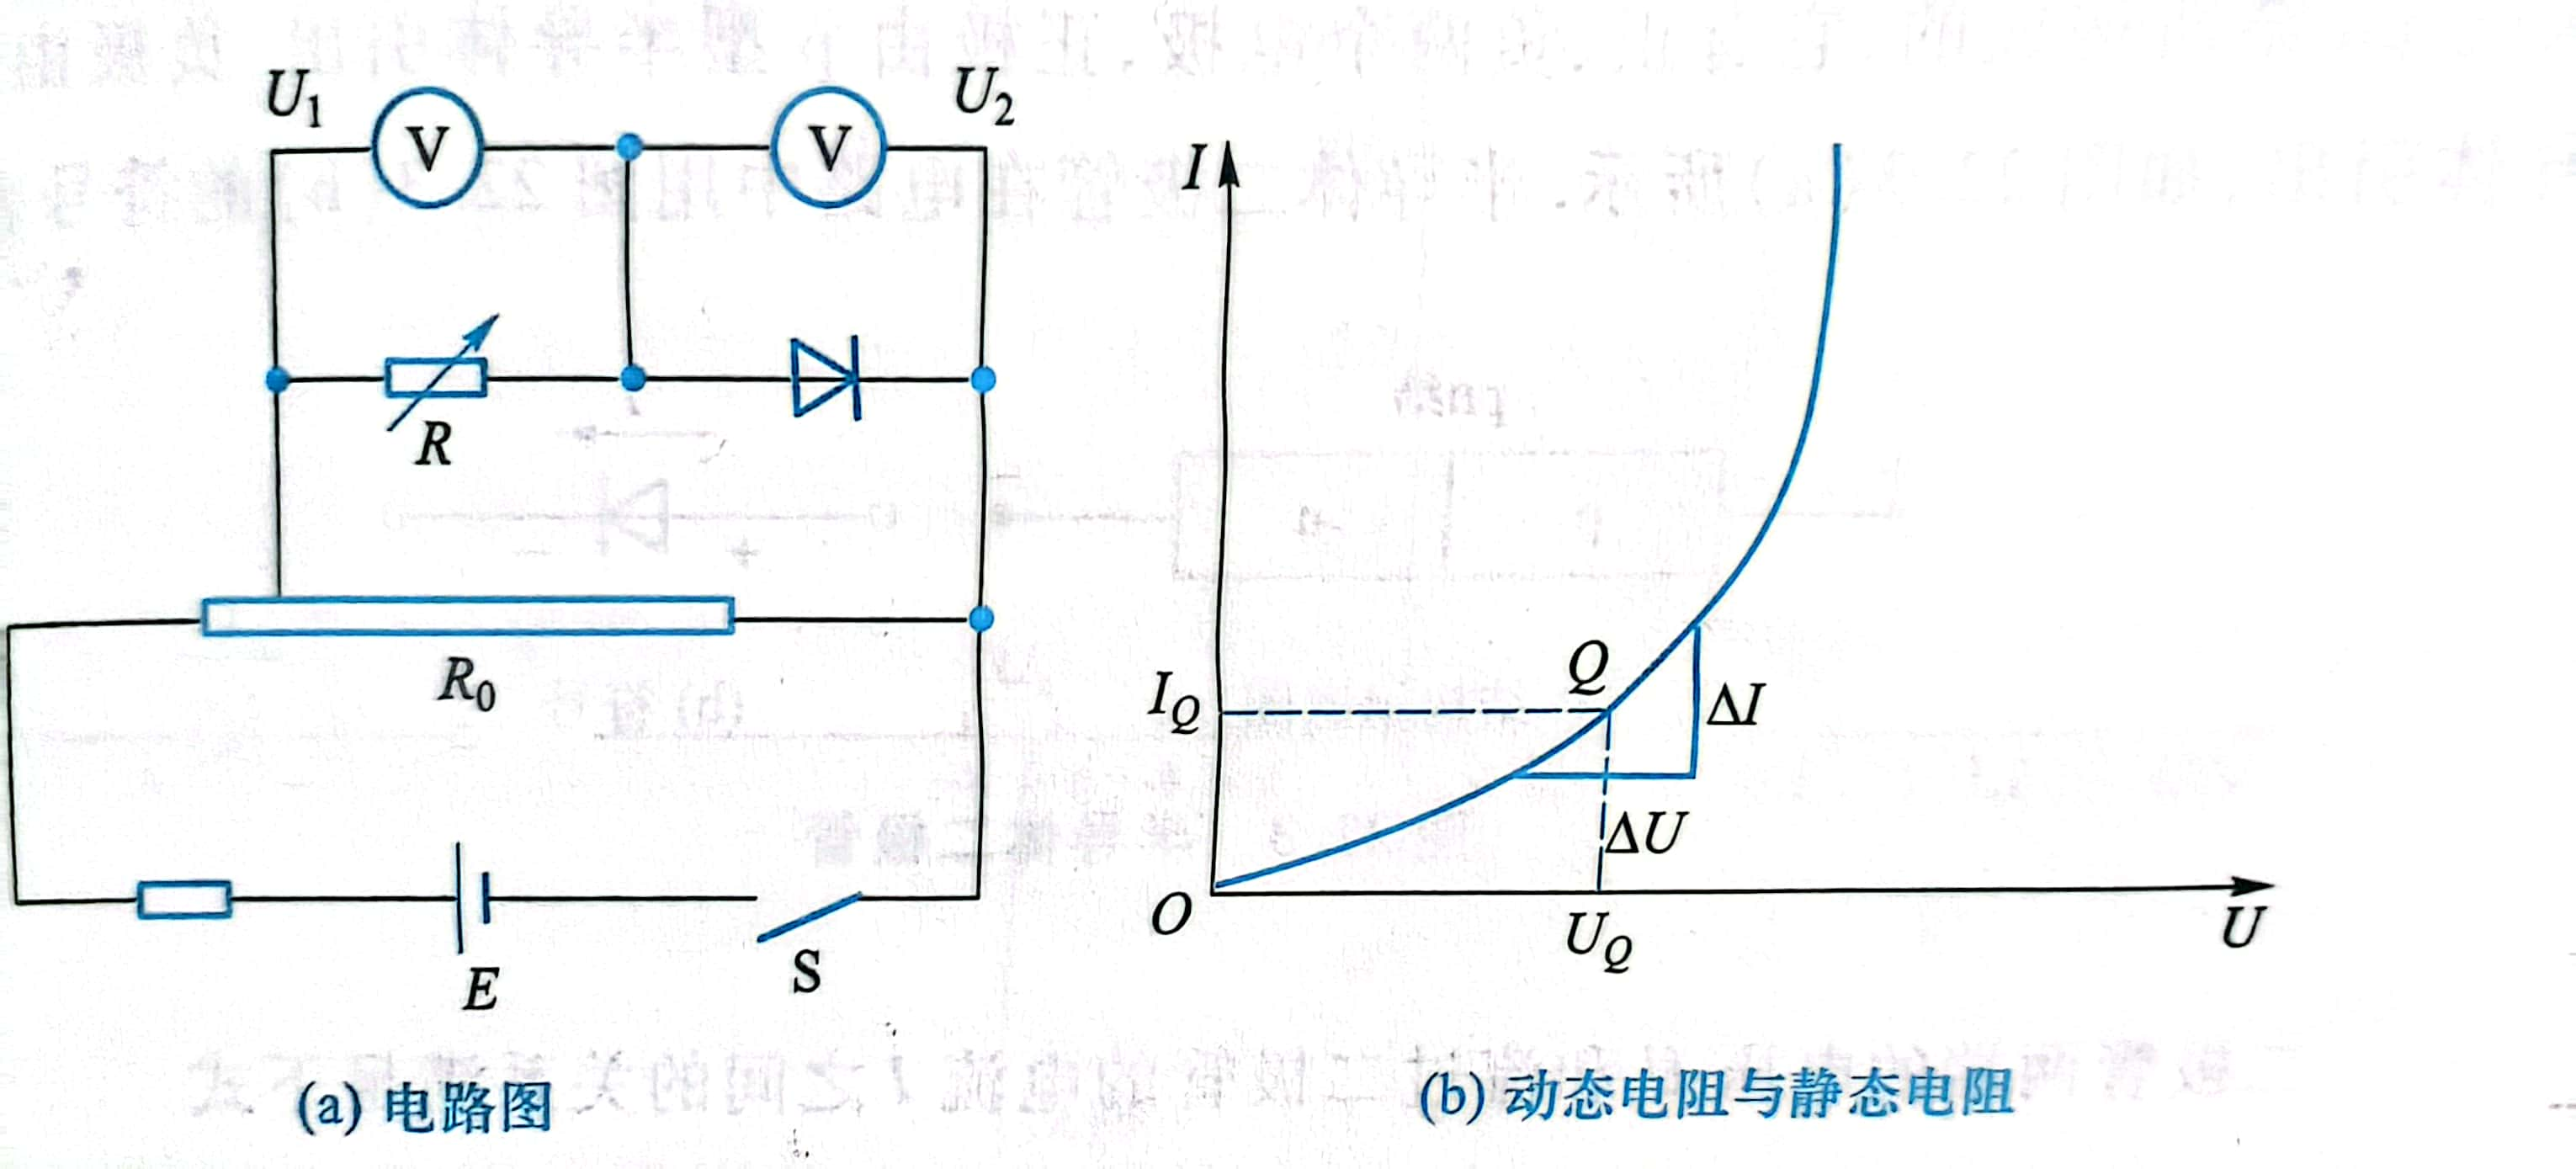
\includegraphics[width=1\textwidth]{fuantexingdianlu.jpg}
    \caption{伏安特性测试电路及非线性元件伏安特性曲线}\label{fuantexingdianlu}
  \end{figure}
  非线性元件的伏安特性可以使用如图\ref{fuantexingdianlu}。电路通过调节$R_{0}$
  来调节$R$以及非线性元件分的电压。再通过$R$的阻值大小来最终控制非线性元件两端
  的电压。电子元件并联的电压表电阻具有较大内阻,在测量这类电阻较低的电子元件的时候
  引入的系统误差较小,可以忽略不计。

  根据欧姆定律$R=\frac{U}{I}$,通过图\ref{fuantexingdianlu}中所展示的电路,由
  待测元件两侧的电压$U$以及电流$I$可以计算得到待测元件的阻值$R$。但是非线性元件的
  阻值$R$并不是一个定值,所以当描述非线性元件的电阻的时候需要指明工作的状态,即指出
  工作电流或者工作电压。

  非线性元件的电阻可用两种方式表示。第一种为静态电阻,用$R_{D}$表示;另一种为动态
  电阻,用$R_{rp}$表示。动态电阻等于工作点附近的电压改变量和电流改变量的比值,可以
  通过伏安特性曲线得到。如图\ref{fuantexingdianlu}展示的那样,在$Q$点附近的
  静态电阻和动态电阻可以表示为
  \begin{equation}
    R_{D}=\frac{U_{Q}}{I_{Q}}
  \end{equation}
  \begin{equation}
    R_{rp}=\frac{\Delta U}{\Delta I}
  \end{equation}

  \subsection{白炽灯灯丝的伏安特性}
  \begin{figure}[t]
    \centering
    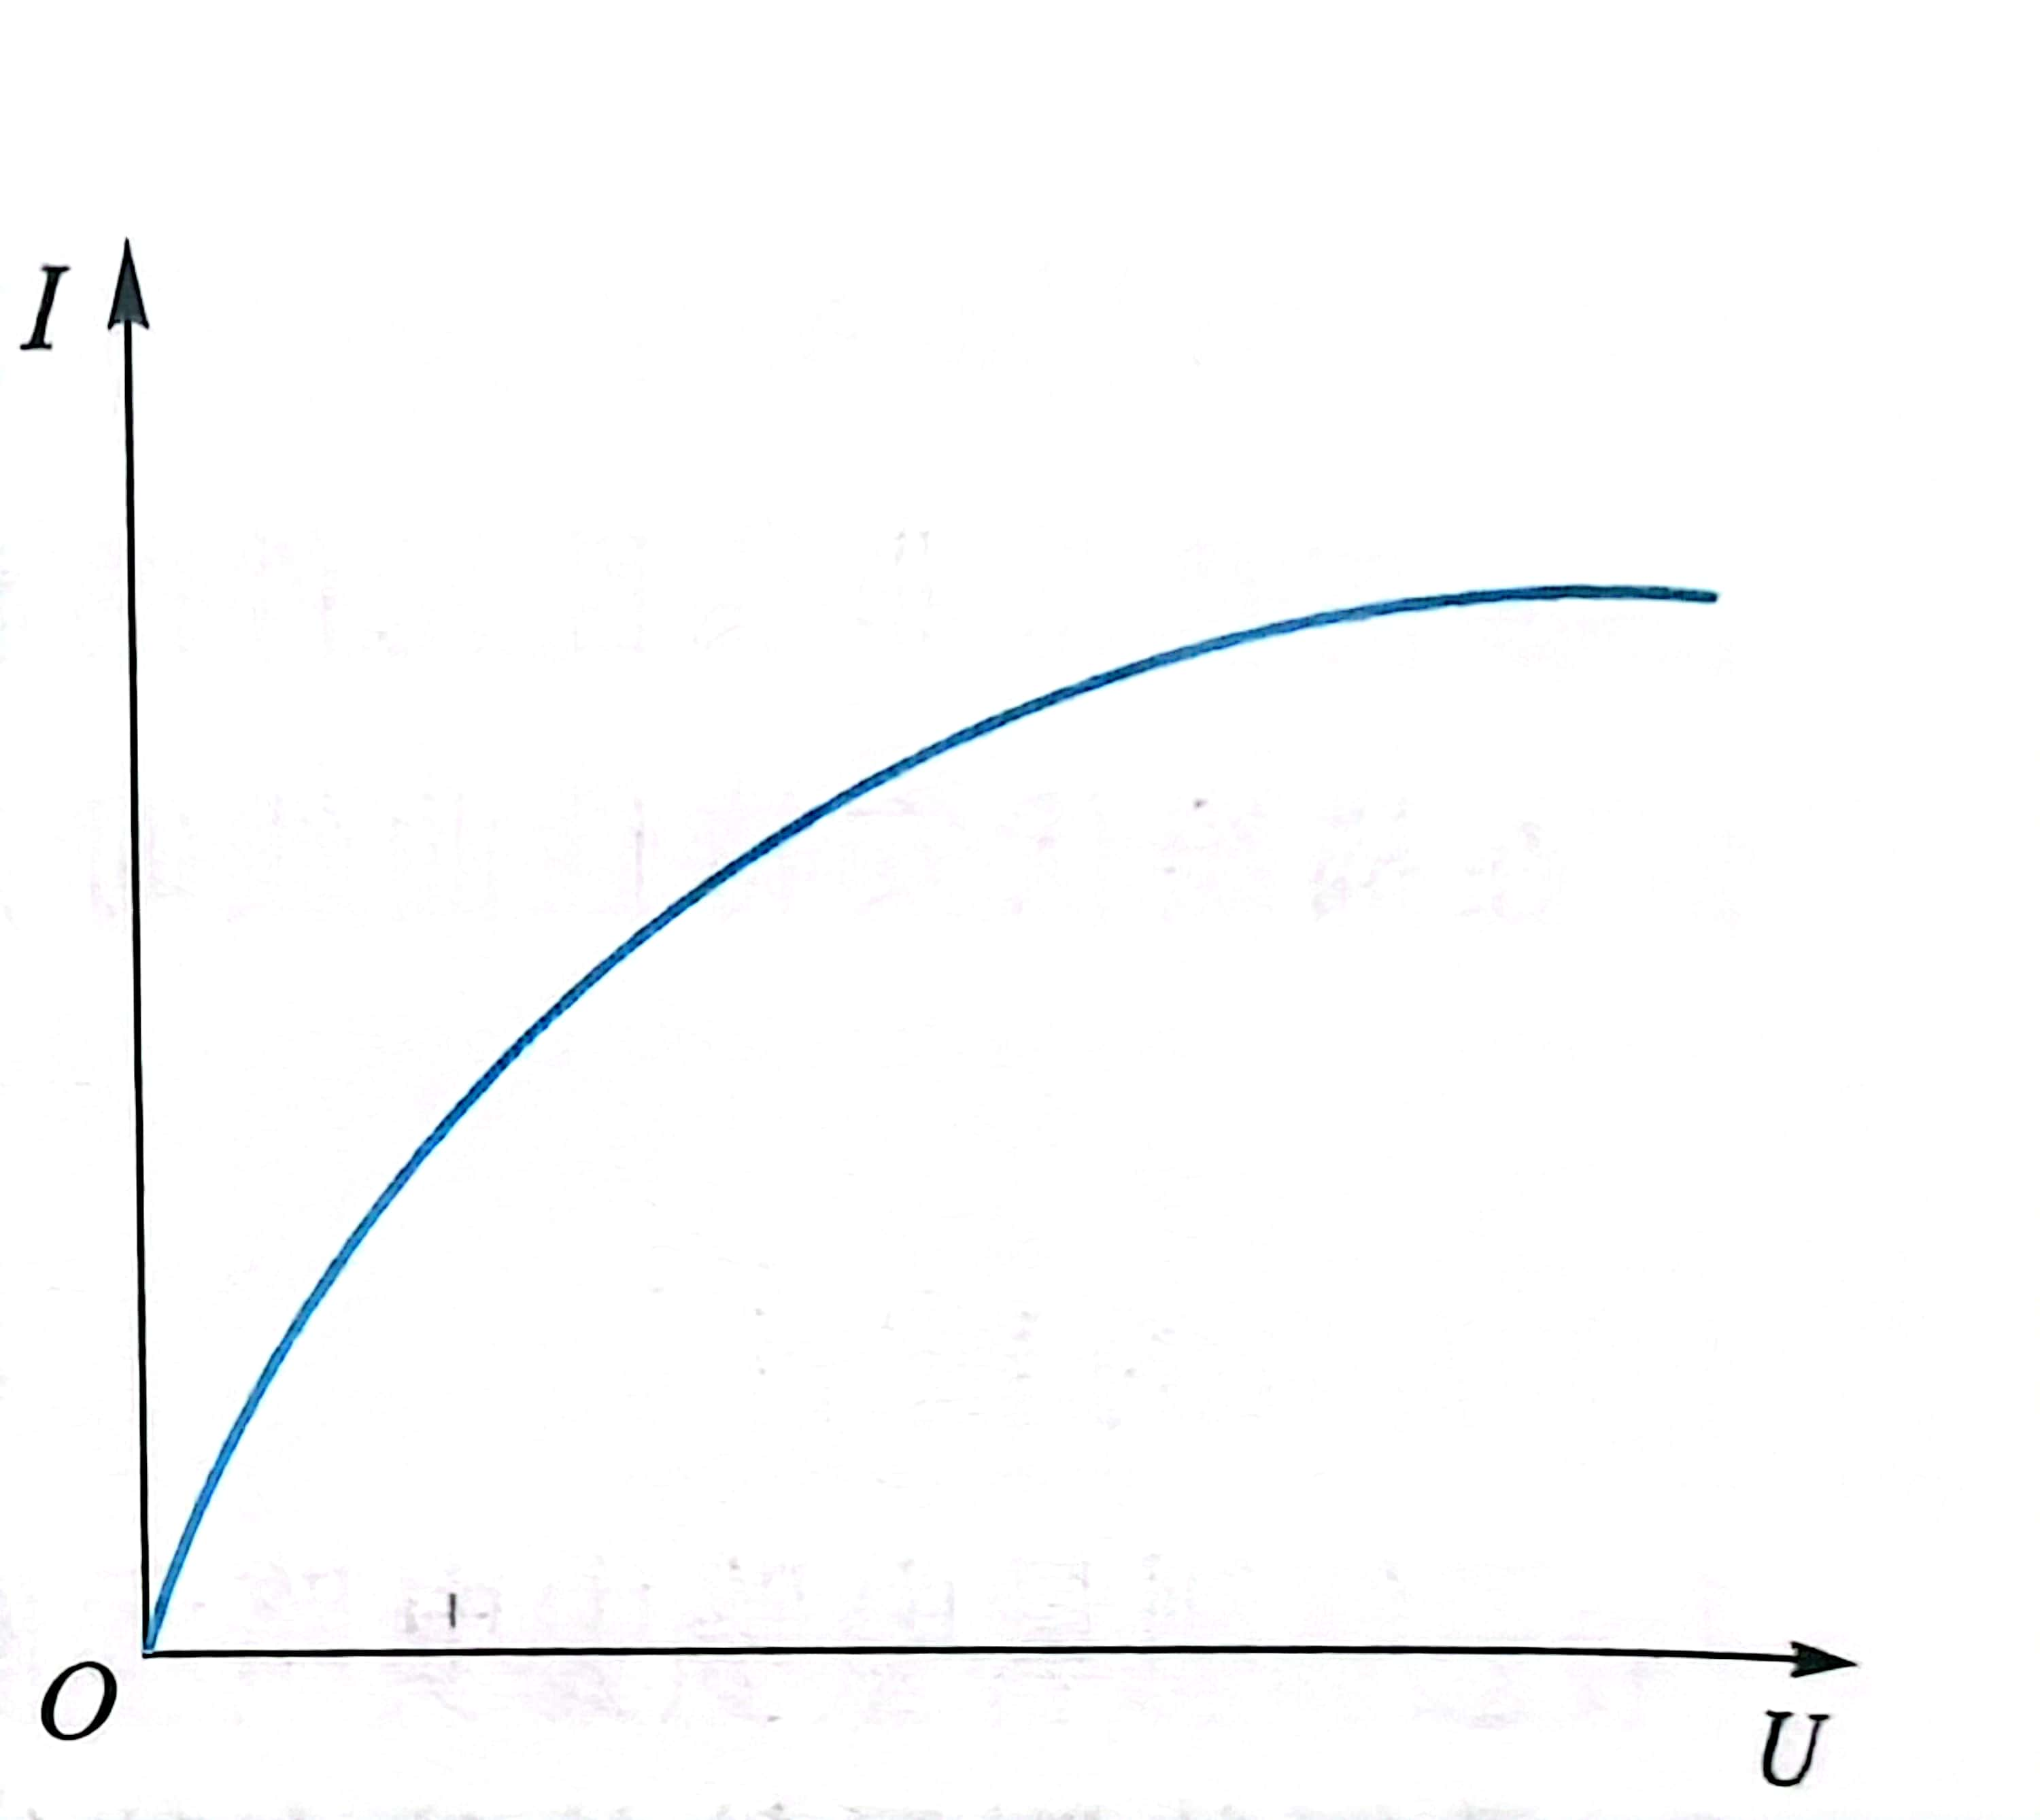
\includegraphics[width=0.5\textwidth,height=0.3\textheight]{dengpaofuantexing.jpg}
    \caption{灯泡伏安特性曲线}\label{dengpaofuantexing}
  \end{figure}
  钨丝类的灯泡发光后,灯丝的电阻会由于发热随着温度升高而增。这意味着通过灯丝的电流越大,
  灯丝发热越严重,电阻也越大。由于温度差异而产生的电阻差异可能相差几倍甚至几十倍。灯泡
  两端的电压以及通过灯泡的电流之间的关系如图\ref{dengpaofuantexing}所示。它们之间的关系
  可以表示为
  \begin{equation}\label{shidengpaofuantexing}
    U=KI^{n}
  \end{equation}
  其中$K$和$n$是和灯泡有关的参数。

  将式\ref{shidengpaofuantexing}两端取对数,将非线性的关系转化为线性关系
  \begin{equation}
    \ln U=\ln K+n\ln I
  \end{equation}
  通过实验测量$U$和$I$关系,再进行作图法或者最小二乘法确定$K$和$n$的值。

  \subsection{半导体二极管的伏安特性}
  \begin{figure}[t]
    \centering
    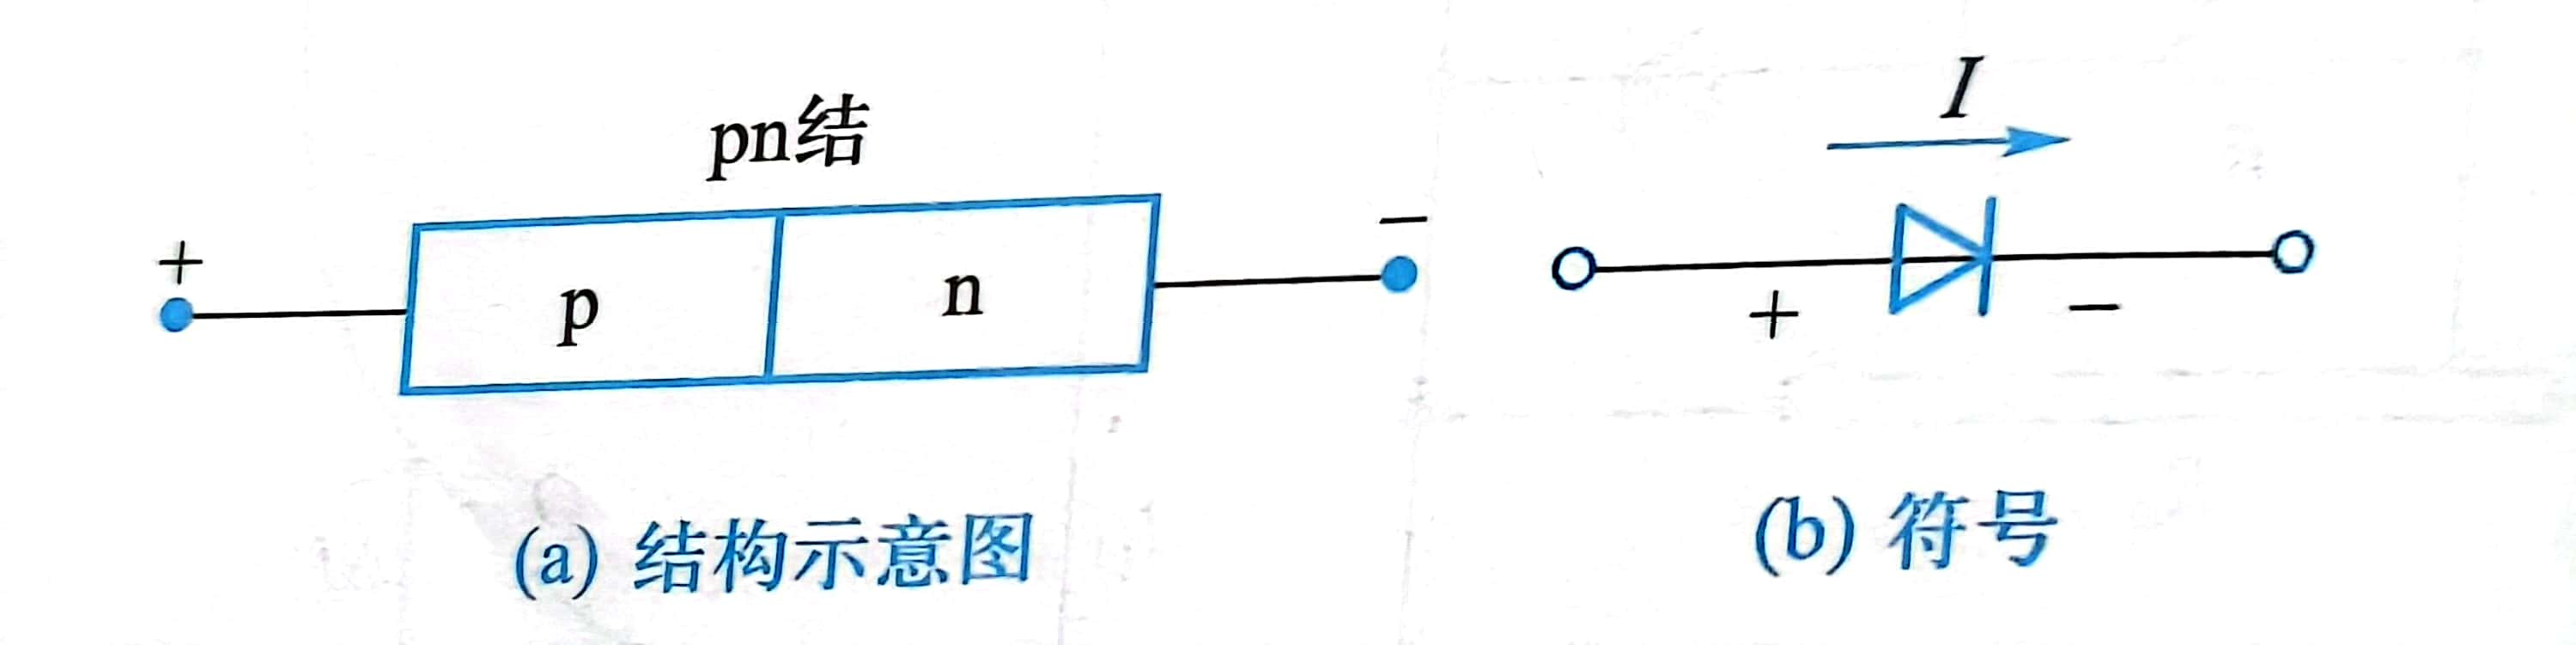
\includegraphics[width=1\textwidth,height=0.3\textheight]{bandaoti.jpg}
    \caption{半导体二极管示意图}\label{bandaoti}
  \end{figure}
    \subsubsection{半导体二极管介绍}
    半导体二极管又称为晶体二极管,也是非线性元件。在电路中二极管具有单向导电性。
    由于能够控制电流流过的方向,所以二极管能够在电路中发挥很多作用,比如整流、检波、
    限幅、元件保护以及数字电路中作为开关的元件。
    二极管是通过两种不同导电性能的半导体进行结合后产生的,这两种半导体分别为
    $n$型半导体以及$p$型半导体。这两种半导体结合后会产生$PN$结。正极由$p$型半导体引出,
    负极由$n$型半导体引出,最终产生的结构以及电路中的示意如图\ref{bandaoti}。
    \begin{equation}\label{erjiguan}
      I=I_{s}(e^{ \frac{qU}{kT}}-1)
    \end{equation}

    \subsubsection{半导体二极管伏安特性}
    二极管两端的电压$U$和流过二极管的电流$I$之间的关系满足式\ref{erjiguan}。
    式子中的$q=1.602\times 10^{-19}C$为电子电荷量的绝对值,
    $k=1.381\times 10^{-23}J/K$为玻尔兹曼常数,$T$为热力学温度,$I_{s}$为反向饱和电流。
    \begin{figure}[tbh]
      \centering
      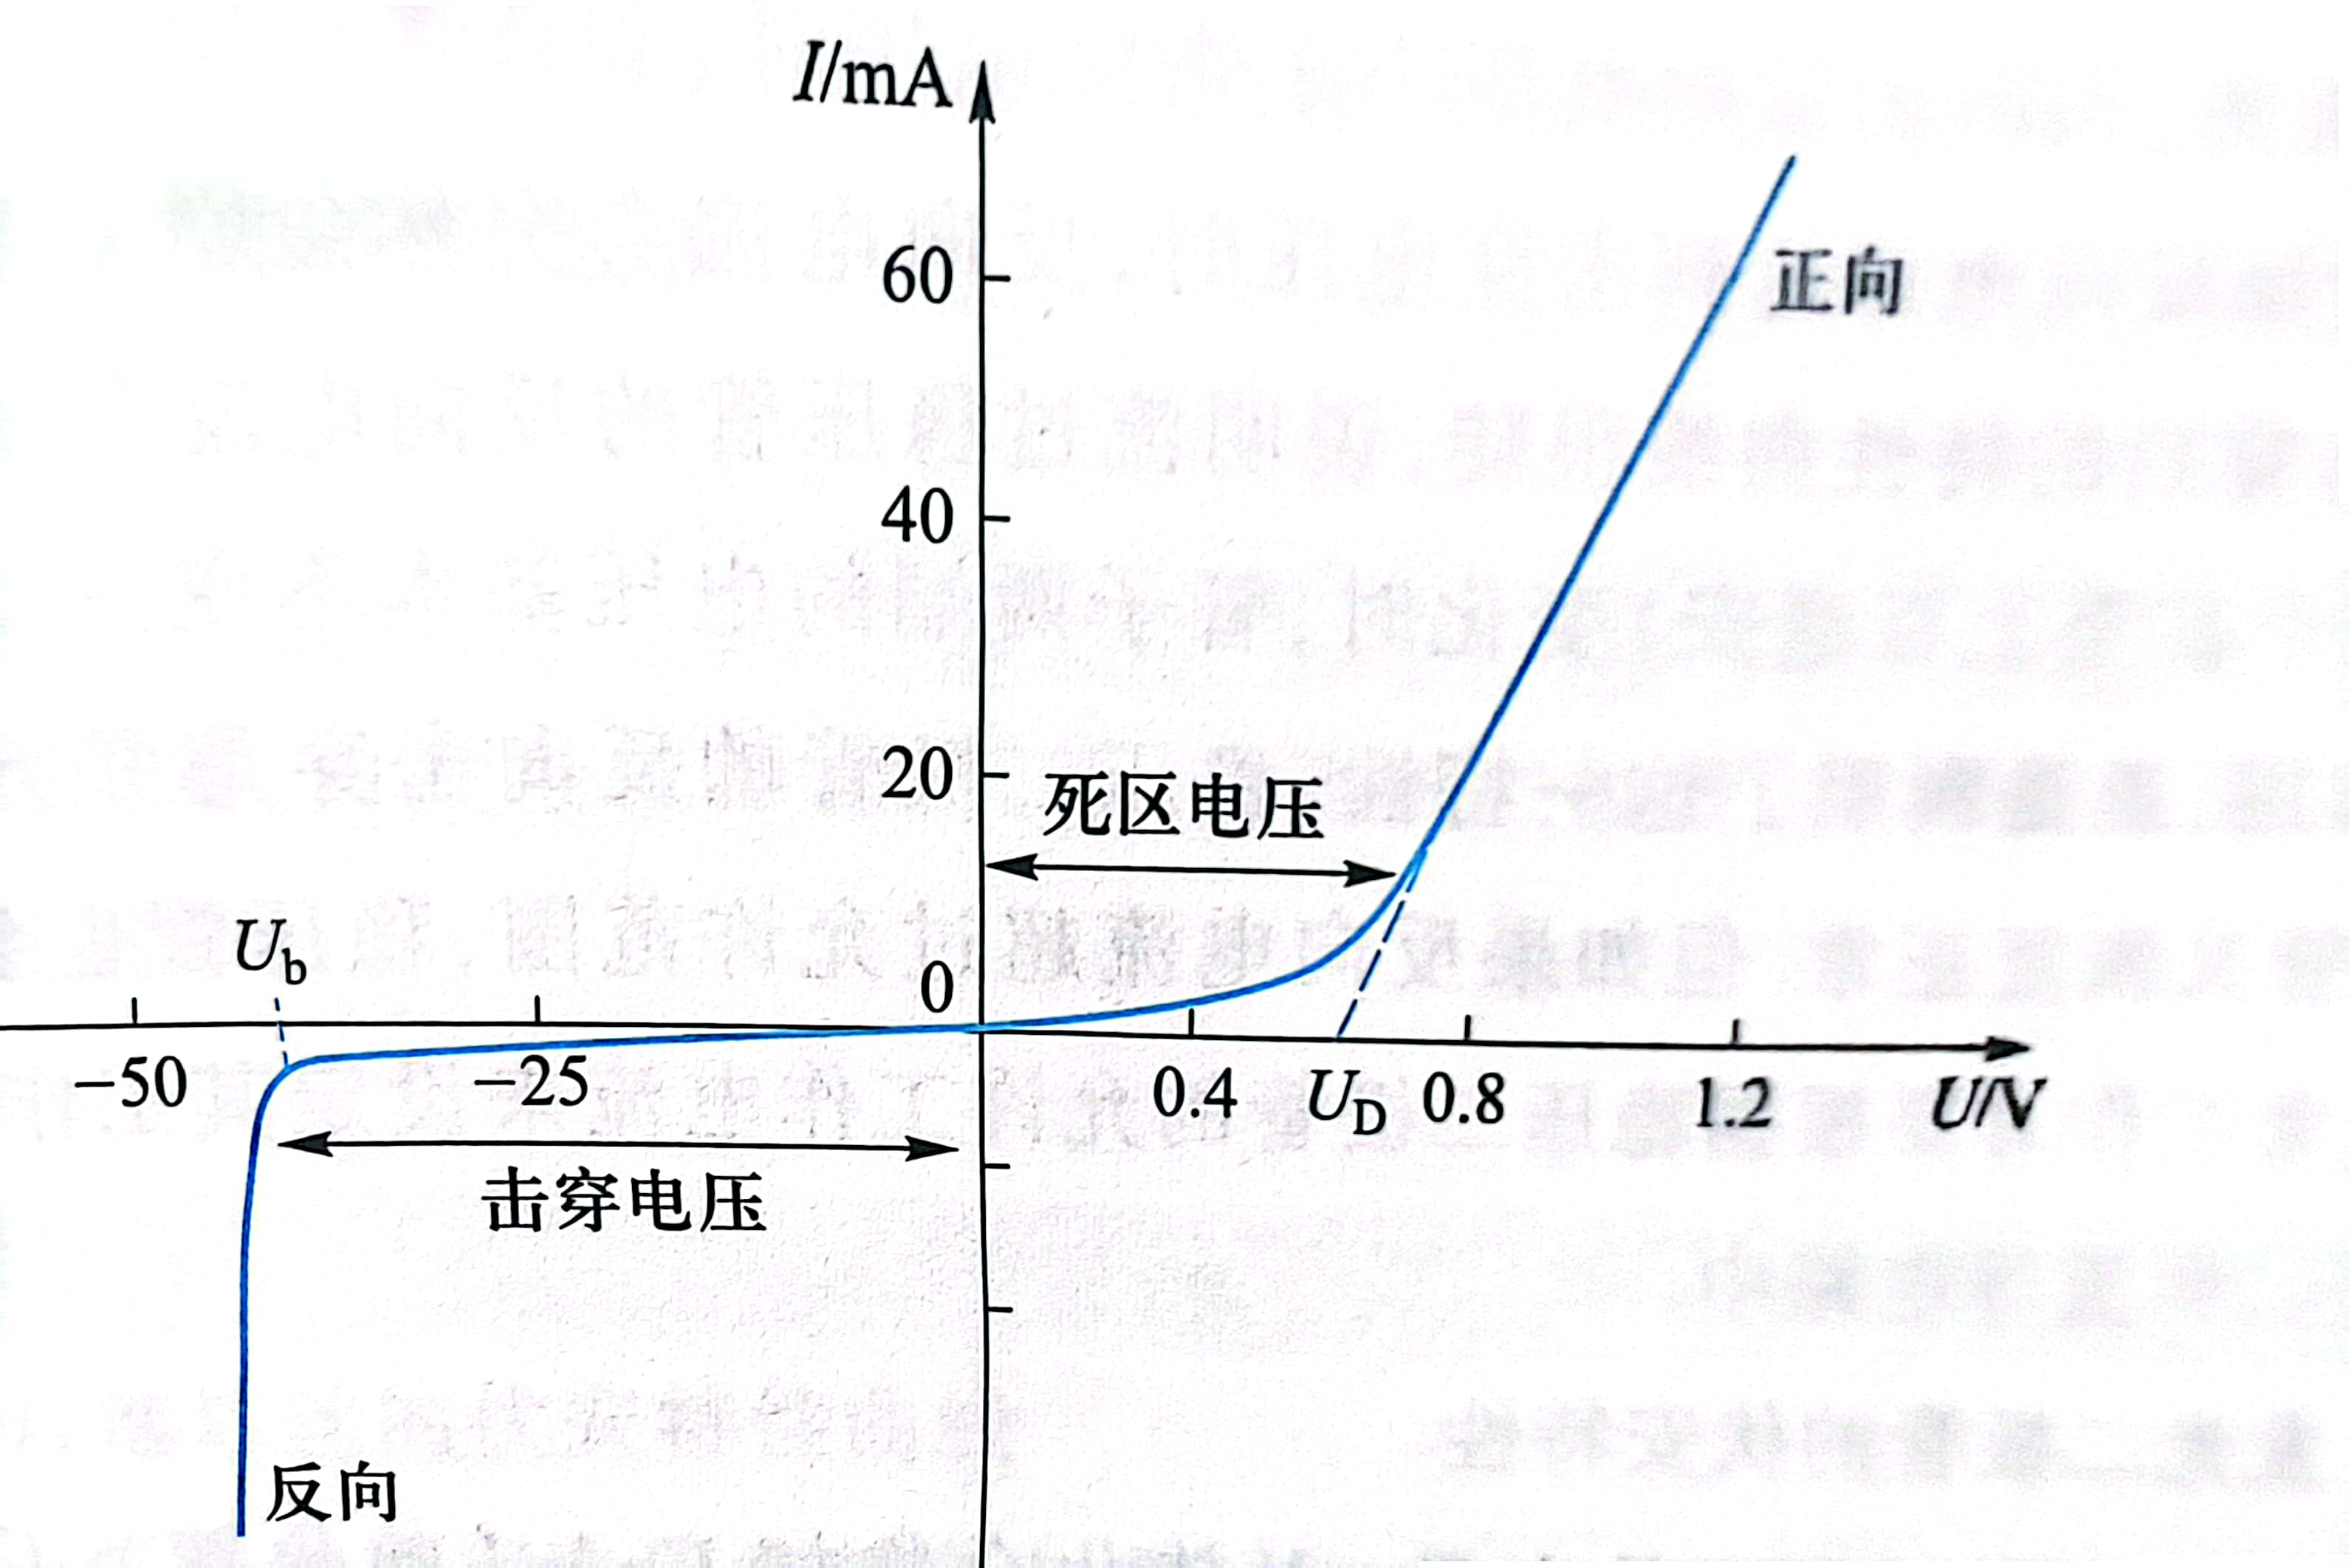
\includegraphics[width=1\textwidth]{erjiguanfuantexing.jpg}
      \caption{半导体二极管伏安特性曲线}\label{erjiguanfuantexing}
    \end{figure}
    
    半导体二极管的主要特点就是单向导电性,其伏安特性曲线如图\ref{erjiguanfuantexing}。由此可以看出,
    二极管在正向电压较小的时候,电流值较小,而一旦电压增加到超过阈值电压$U_{D}$之后,正向电流开始明显
    增大,随着电压增加电流也在急速增大,伏安特性曲线近似可以看为一条直线。将该直线反向延长和$x$轴
    相交于$U_{D}$,$U_{D}$为正向导通阈值电压

    而对半导体二极管加上反向电压的时候,反向电流极小而且随电压变化缓慢,但当反向电压最终超过击穿
    电压时候$U_{b}$,电流将急剧增大,二极管被击穿后仍可以恢复到正常工作,但是由于发热等原因实际上
    仍然会对二极管产生不可逆的损害,最终造成二极管永久损坏。

  \subsection{稳压二极管的伏安特性}
  稳压二极管是一种特殊的硅二极管,伏安特性曲线如图\ref{wenyafuantexing}
  \begin{figure}[tbh]
    \centering
    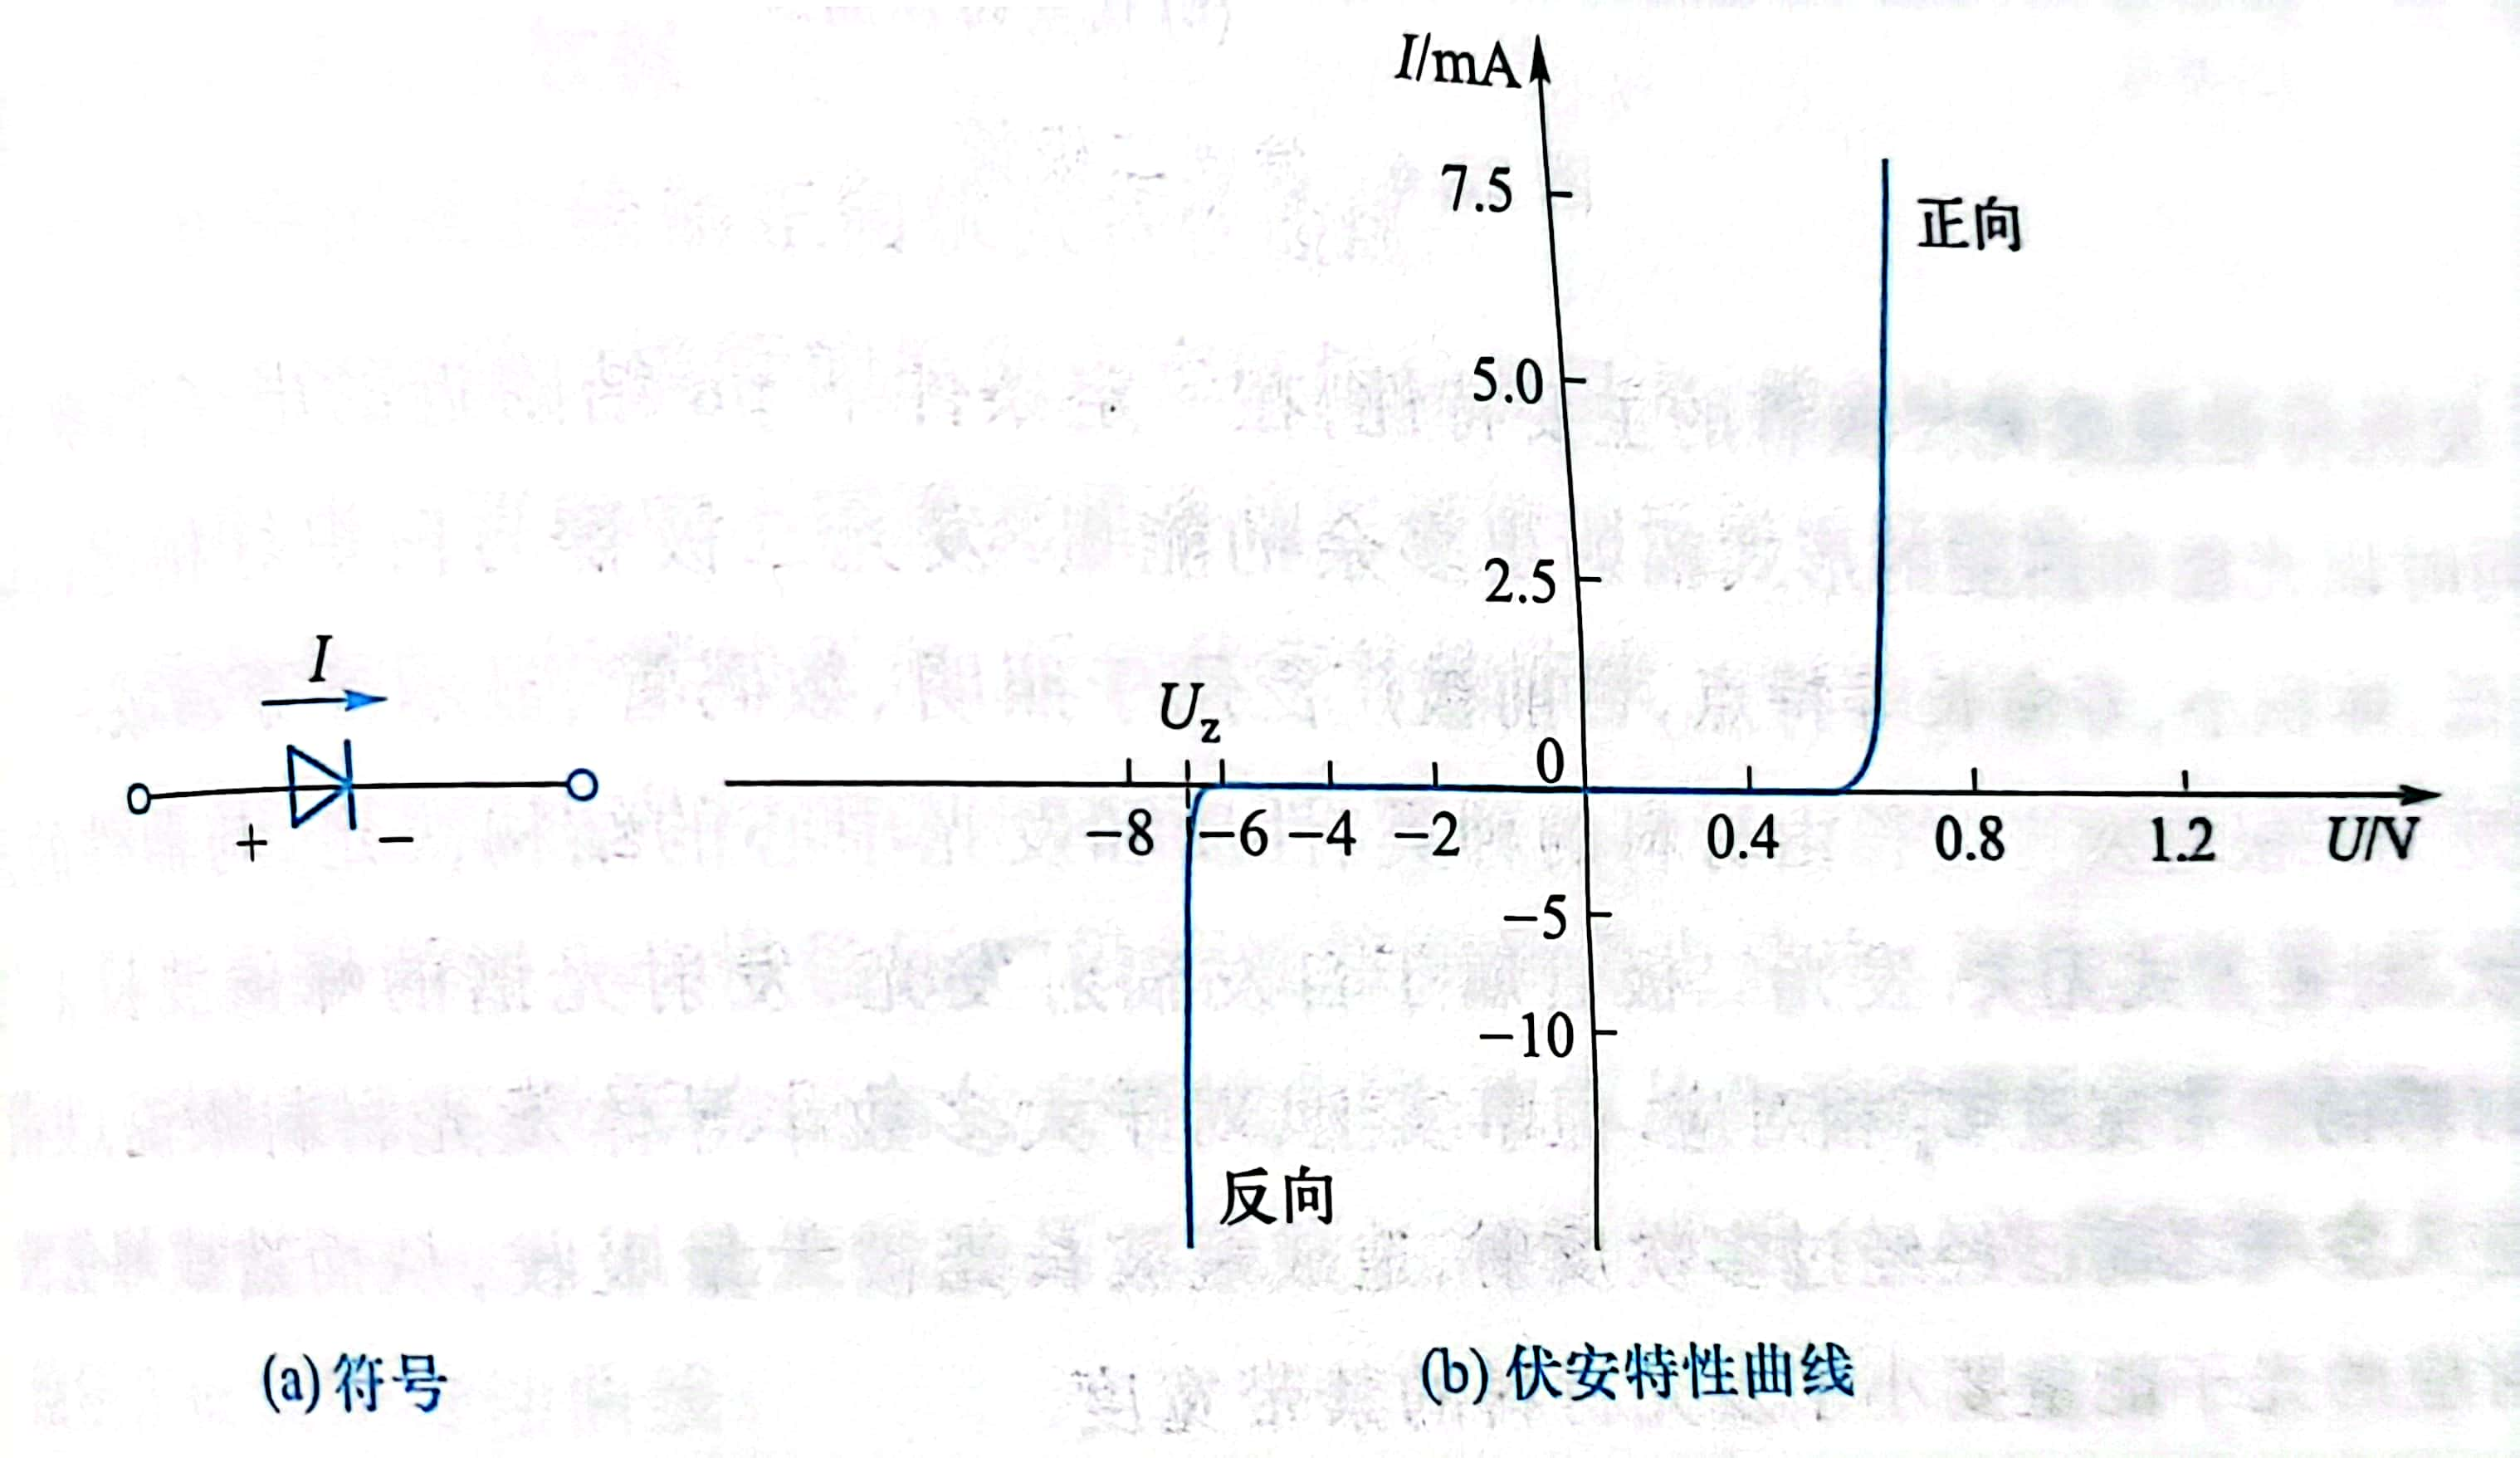
\includegraphics[width=1\textwidth]{wenyafuantexing.jpg}
    \caption{稳压二极管伏安特性曲线}\label{wenyafuantexing}
  \end{figure}
  稳压二极管的伏安特性曲线和普通二极管的和普通二极管类似,只是反向特性曲线较普通二极管更陡。

  对于稳压二极管而言,当电压小于反向击穿电压的时候,它和普通二极管一样。但是一旦电压大于反向击穿
  电压,则在电压增加一个微小量后电流将产生巨大的变化,这说明在很大的电流范围内需要的电压是近似
  不变的。因为这个特性,稳压二极管可以在电路中作为稳压的器件。同时稳压二极管的反向击穿是可逆的,
  当反向击穿电压消失后稳压二极管优惠回复正常。但是和普通的二极管一样,反向击穿是有允许的电压范围的,
  稳压二极管也是一样,如果反向电流超过的了允许范围,则稳压二极管会一样一位电流过大而发热而损坏。
  
  由于具有以上特性,稳压二极管一般用在稳压或者恒流的电路中。

  \subsection{发光二极管的伏安特性}
  \begin{figure}[t]
    \centering
    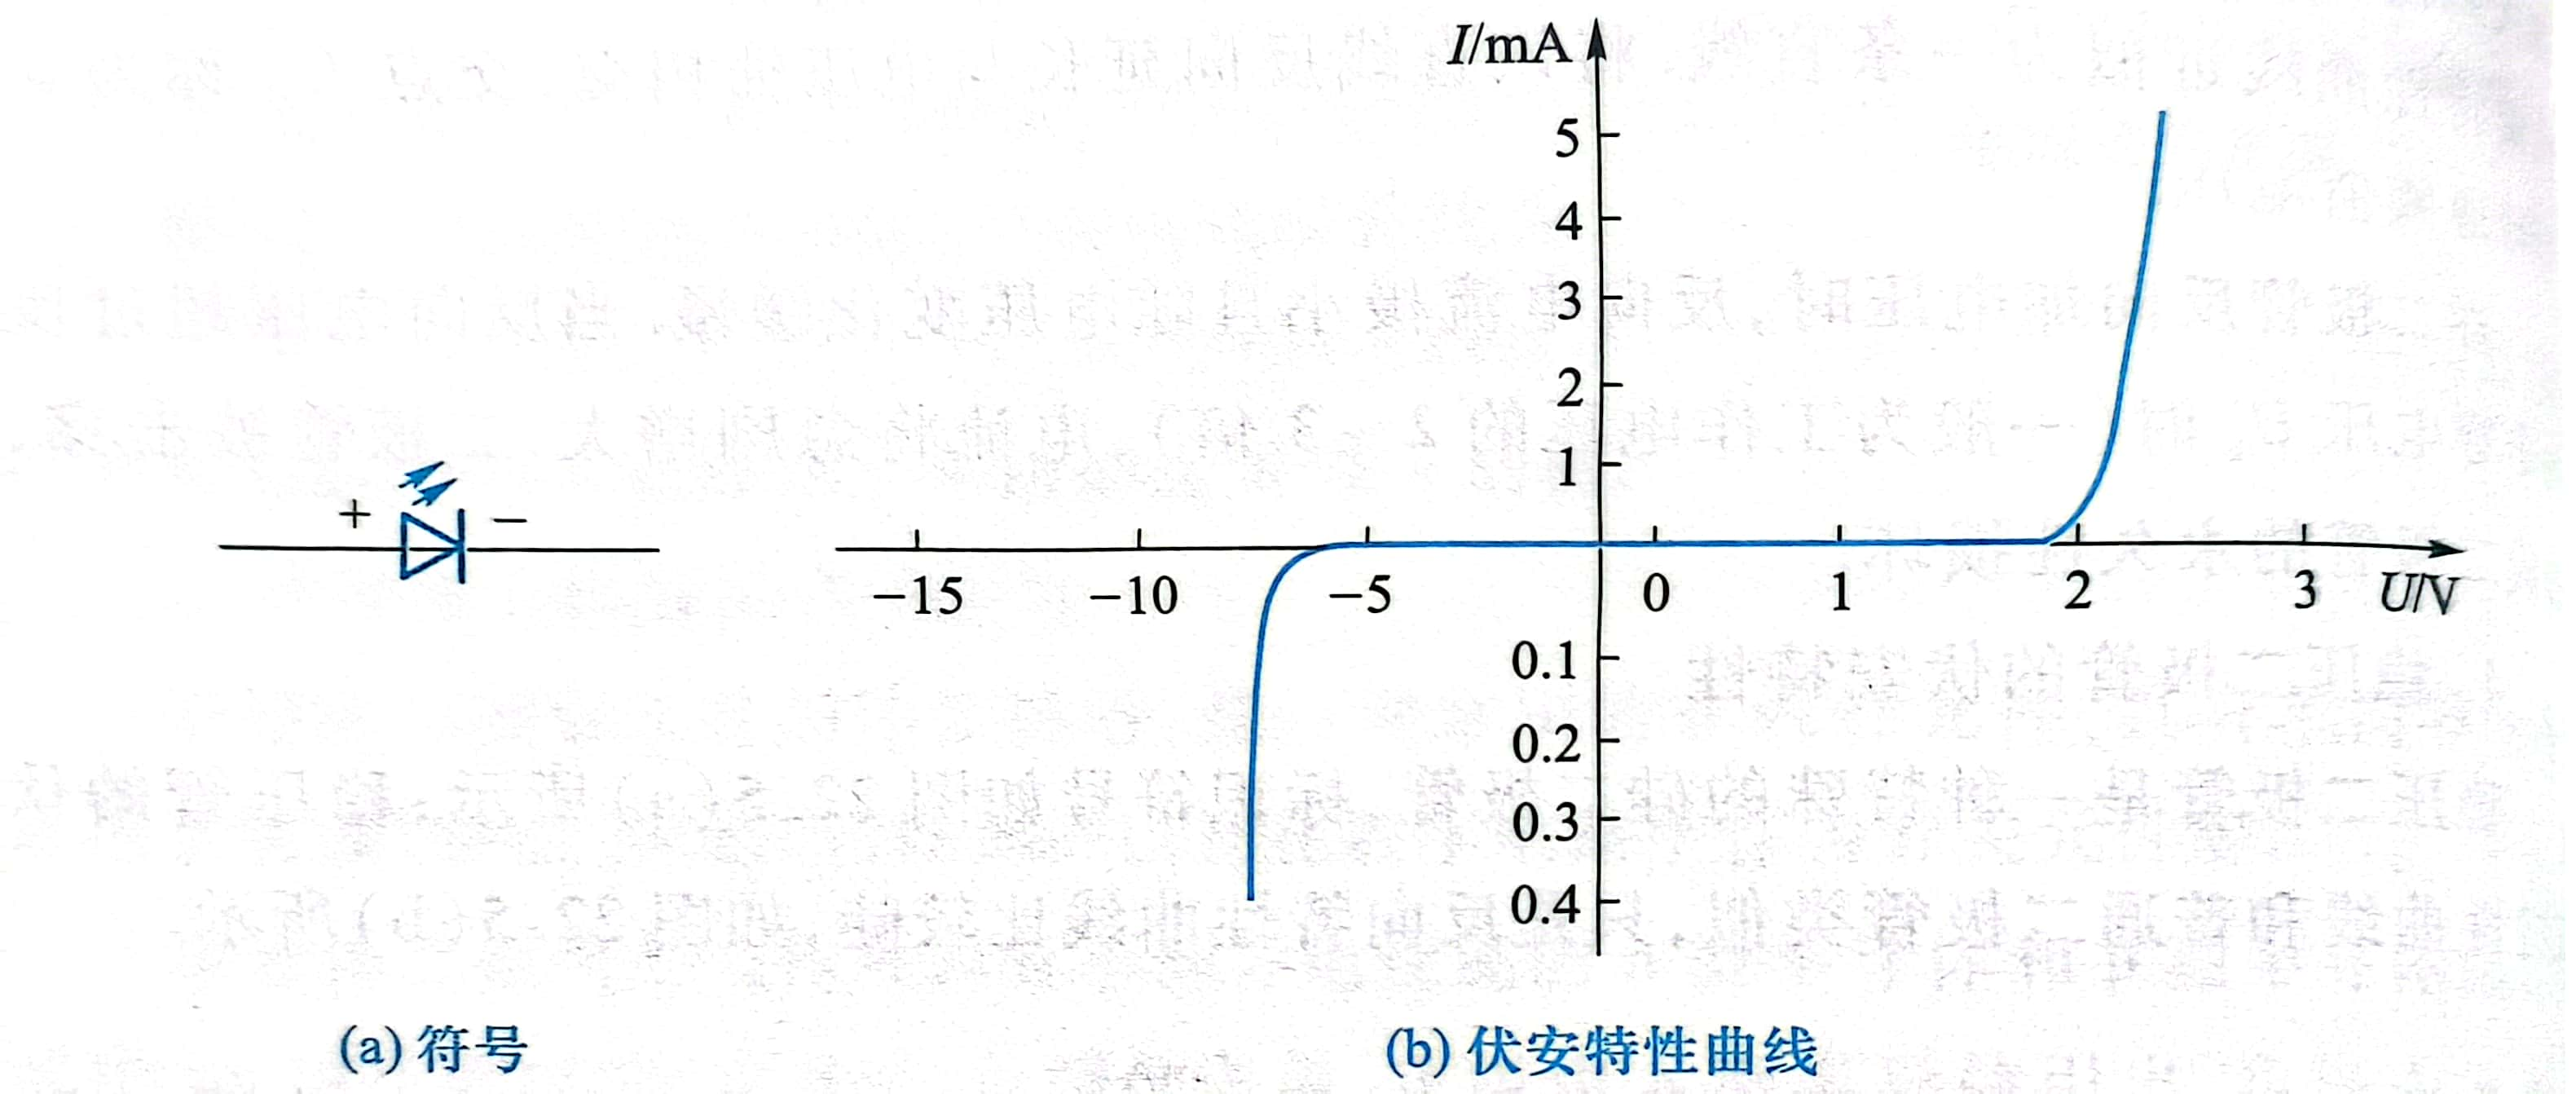
\includegraphics[width=1\textwidth]{faguangfuantexing.jpg}
    \caption{发光二极管伏安特性曲线}\label{faguangfuantexing}
  \end{figure}
  发光二极管,也就是常说的LED一般是由$III-V$族化合物如$GaAs$、$GaP$、$GaAsP$等半导体材料制成的,发光二极管在电路中的符号如
  图\ref{faguangfuantexing}中展示的那样。发光二极管的核心依旧是pn结,因此它具有一般pn结有的特性,它的伏安特性曲线和普通的
  二极管类似。
  
  发光特性是发光二极管的主要特性,在一定条件下pn结附近的的电子和空穴会复合,同时以光能和热能的形式向外辐射出多余的能量。发光
  二极管和白炽灯相比,具有功耗低,体积小,寿命长的特点,目前被广泛应用在照明、数码管、显示屏等电子领域。

  对于发光二极管而言,发光的波长由材料的种类、性质和发光中心的结构相关。但是和器械的封装方式、形状无关。发光二级管属于
  自辐射发光,所以发射光谱的峰值波长$\lambda$和发光材料的禁带宽度$E_{g}$相对应。但是事实上对于大多数半导体发光材料而言,发射光进入
  空气之前已经经历了多次反射,所以造成了短波长光被大量吸收,从而造成峰值波长相对应的光子能量要小于发光材料的禁带宽度。

  辐射跃迁所发出的光子的峰值波长$\lambda$可以由式\ref{fenzibochang}来计算
  \begin{equation}\label{fenzibochang}
    \lambda \approx 1240/E_{g} \quad (nm)
  \end{equation}

\section{实验装置器材介绍}
稳压电源、电阻箱、可变电位器、九孔板、待测试二极管、待测试稳压二极管、待测试小灯泡、导线若干

\section{实验内容及实验步骤}
  \subsection{测量普通电阻通电后的伏安特性曲线}
  连通电路,测量在不同电压下流过电阻的电流大小。
  并记录实验数据,绘制图像观察直线斜率和电阻阻值大小。

  \subsection{测量普通二极管的正向伏安特性曲线}
  \begin{figure}[b]
    \centering
    \begin{minipage}[b]{0.48\textwidth}
      \centering
      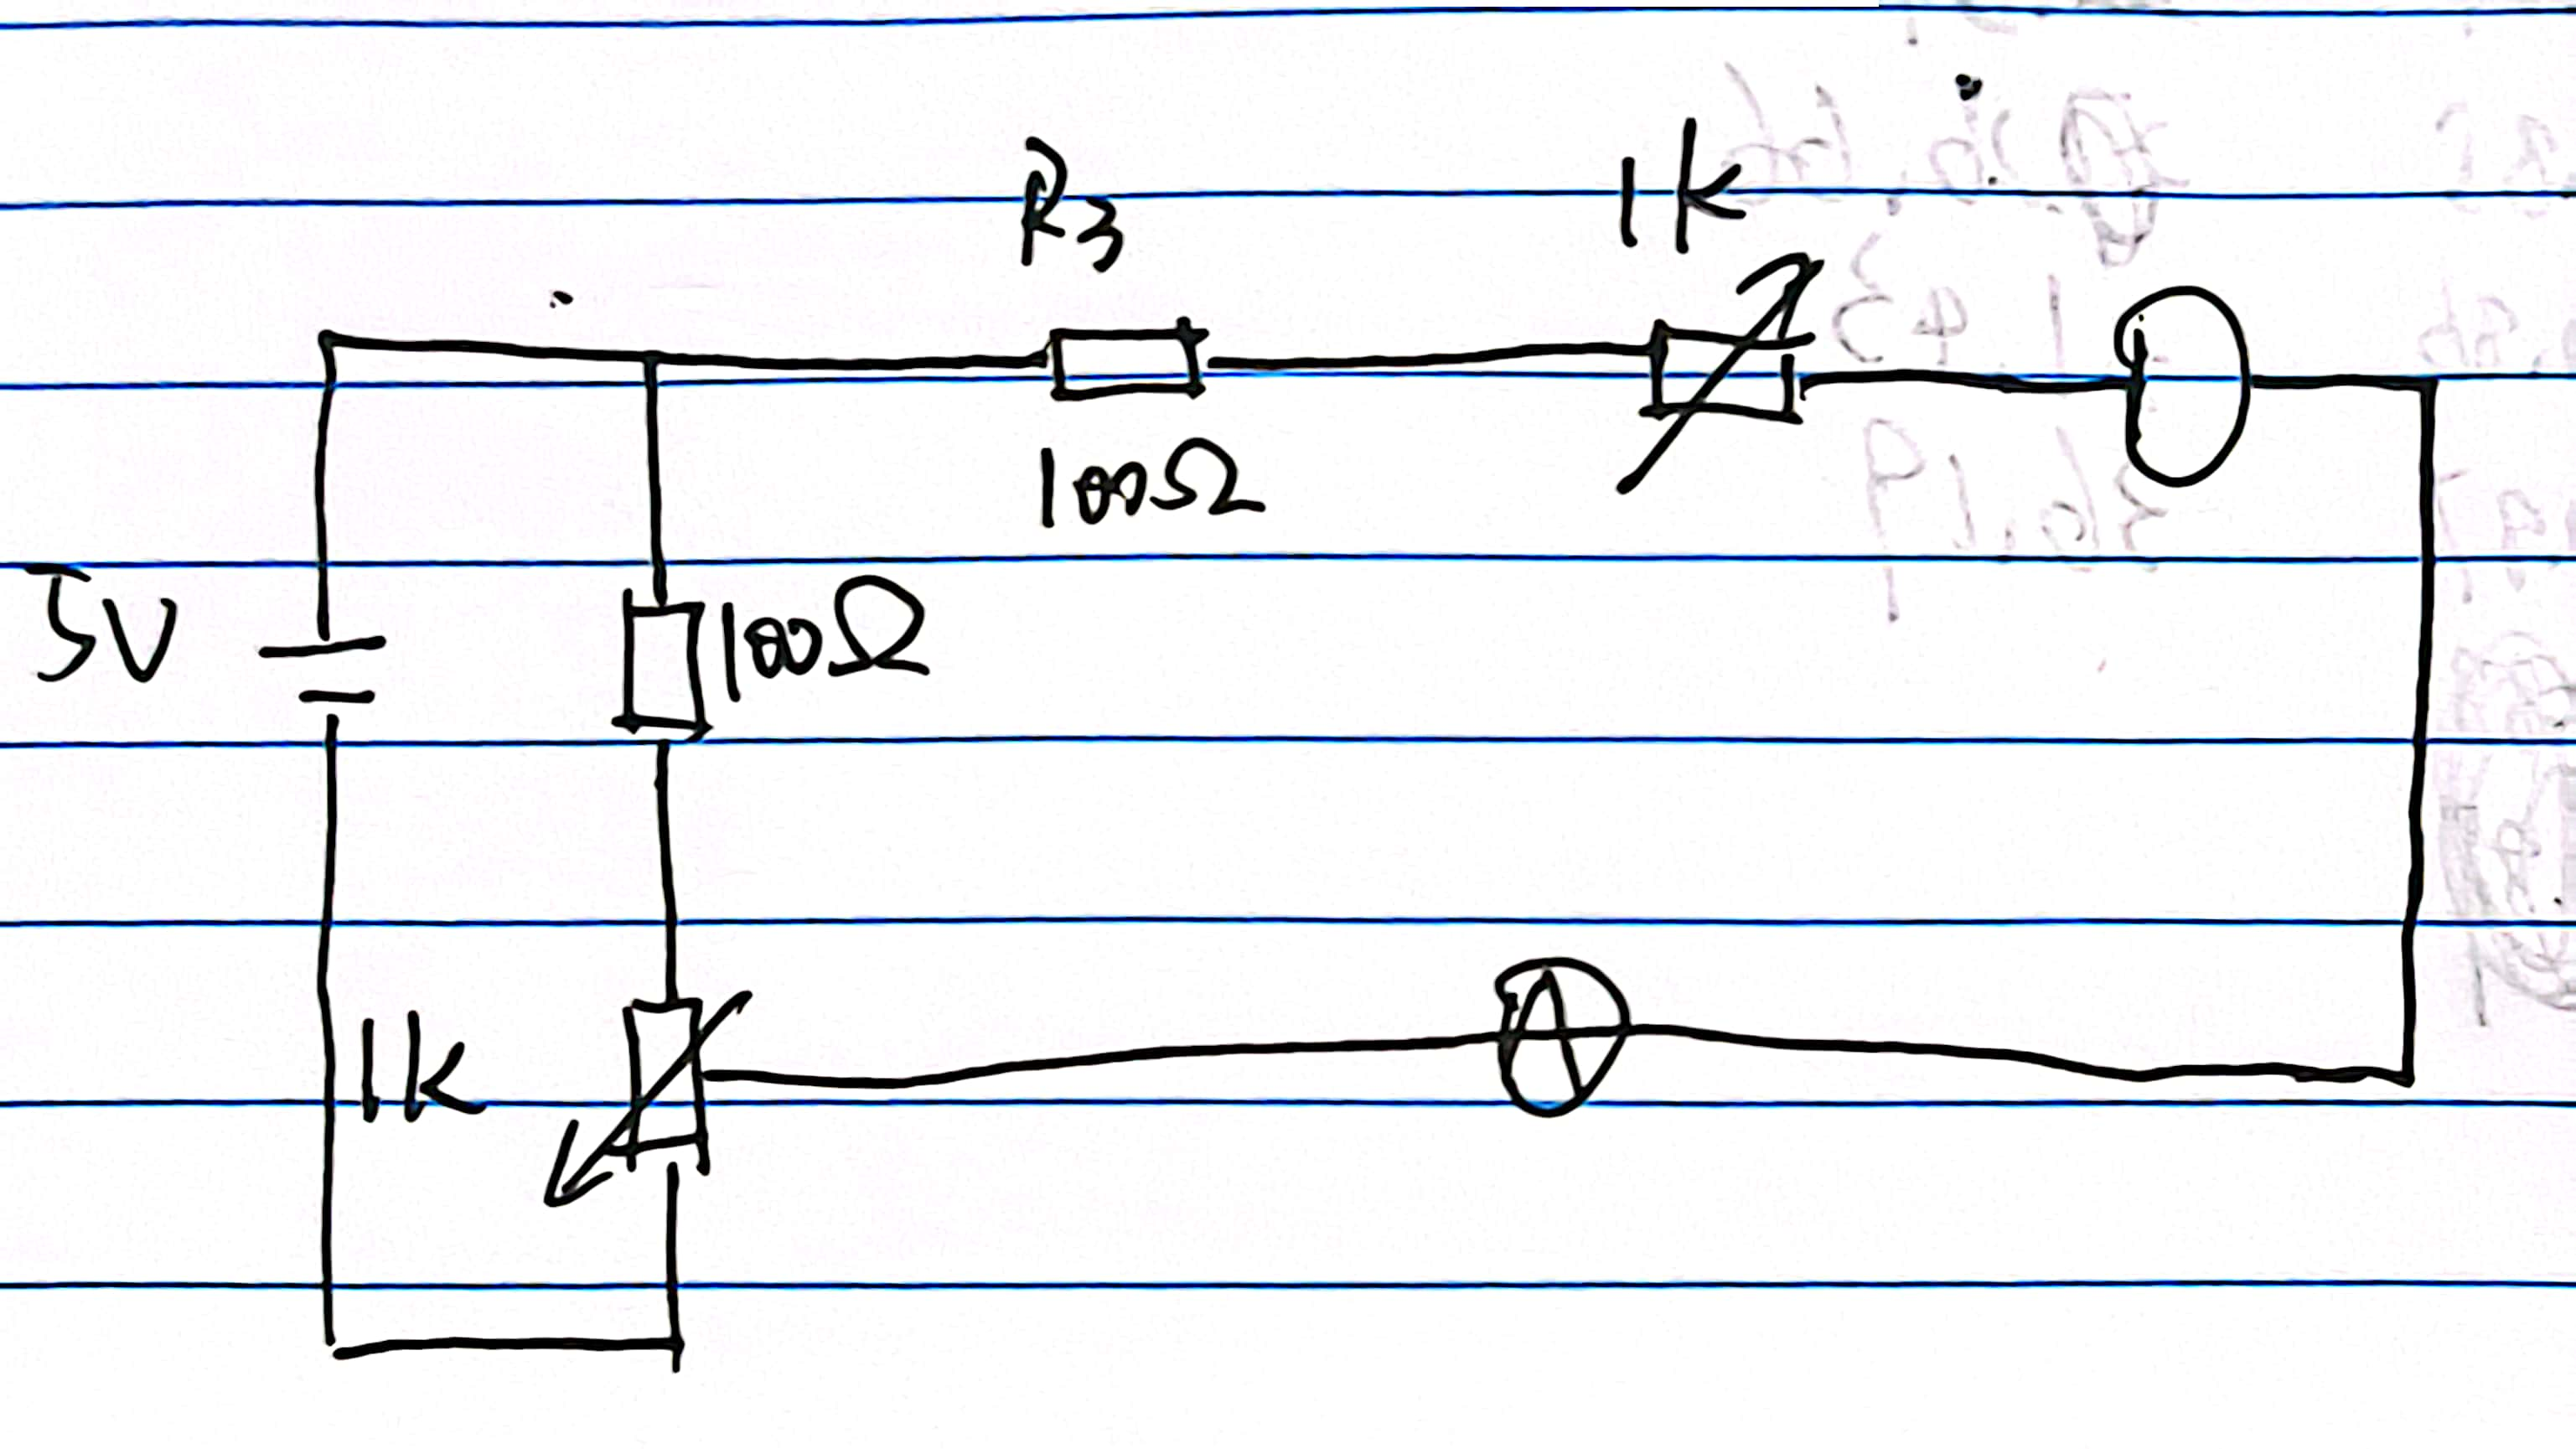
\includegraphics[width=0.46\textwidth]{zhengxiangdianlu.jpg}
      \caption{二极管正向连通电路示意图}\label{zhengxiangdianlu}
    \end{minipage}
    \begin{minipage}[b]{0.48\textwidth}
      \centering
      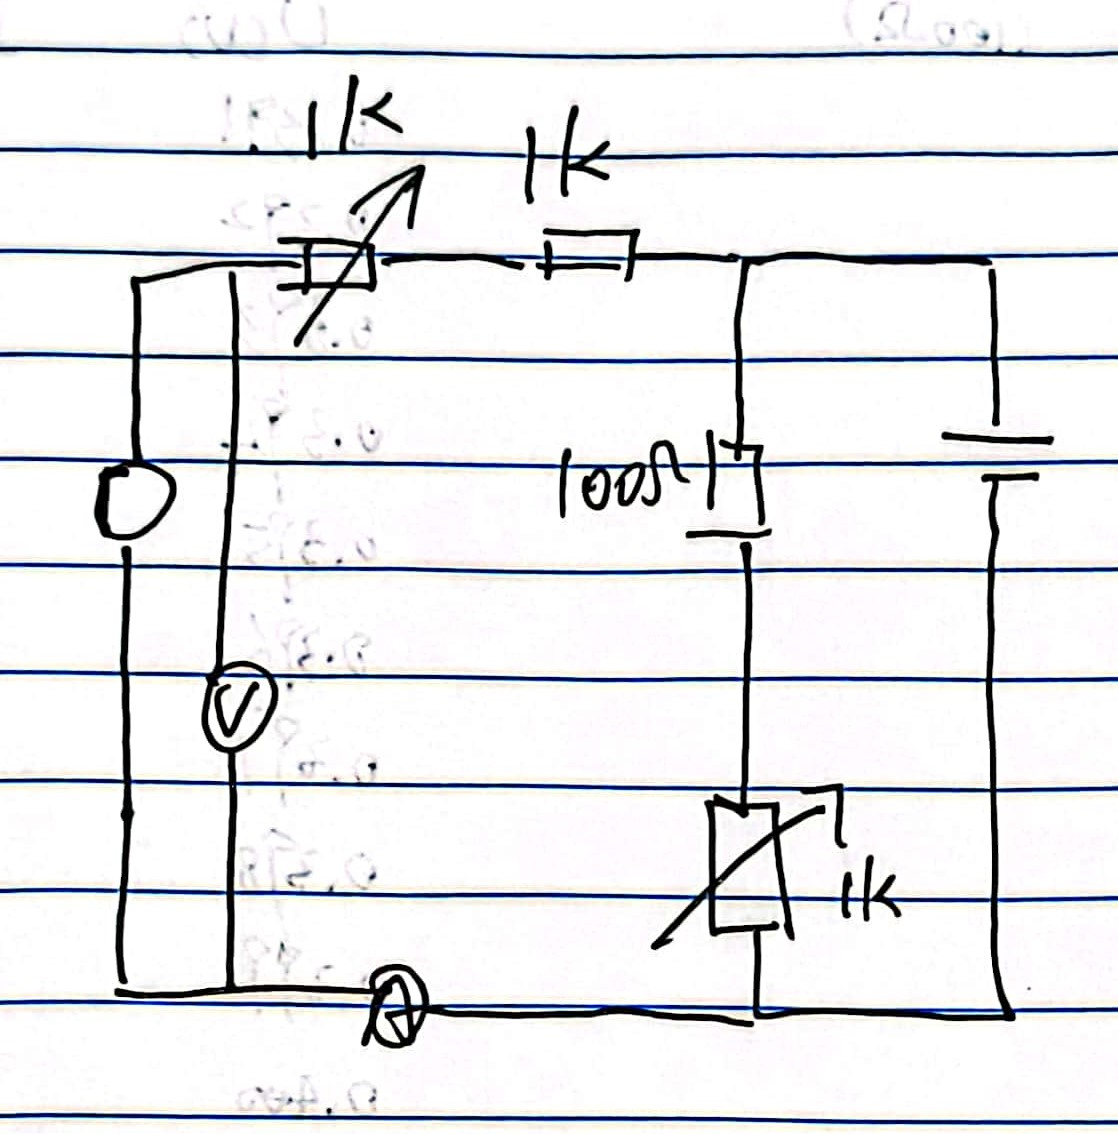
\includegraphics[width=0.46\textwidth]{fanxiangdianlu.jpg}
      \caption{二极管反向连通电路示意图}\label{fanxiangdianlu}
    \end{minipage}
  \end{figure}

  \(1\) 先使用数字多用表判断二极管的正负极。具体操作如下\\
  将数字多用表调节到二极管挡位,红黑表笔分别链接二极管的两端,观察万用表的示数。\\
  交换红黑表笔,在观察示数。\\
  若显示为0.7V左右电压,则表示红表笔一端为二极管的正极,另一端为负极。\\
  若反向链接,则显示为短路状态。\\
  若正反两个方向测得的结果一致,则表明该二极管已损坏。

  \(2\) 按照图\ref{zhengxiangdianlu}连接电路,将普通二极管连入伏安特性测量电路中。连接的时候注意
        正负极链接电源是否正确。调节电压,从0开始缓慢增加,观察电流。其中电流不要超过20mA,以免烧坏二极管。
        实验中需要测试15组数据。

  \(3\) 在作图纸上绘制正向伏安特性曲线。

  \(4\) 补充:最终实验没有测试反向击穿电压的原因是因为普通的二极管的反向击穿电压一般达到100V,远远超出了安全
        电压的范围,因此实验中不需要测量普通二极管的反向击穿电压。

  \subsection{测量稳压二极管的正向、反向伏安特性曲线}
  \(1\) 用数字多用表判断稳压二极管的正负极。
  
  \(2\) 按照图\ref{zhengxiangdianlu}连接电路,注意电流正向导通。测量15组数据

  \(3\) 按照图\ref{fanxiangdianlu}链接电路,注意电流反向导通。测试稳压二极管反向击穿电流特性。注意
        电流不要超过30mA,测量15组数据。测量反向击穿电压。

  \(4\) 在做图纸上作图得到伏安特性曲线。

  \subsection{测量发光二极管正向伏安特性曲线}
  \(1\) 参照普通二极管的实验步骤进行实验。测量15组数据。

  \(2\) 总共需要进行三个发光二极管的数据的测量和计算。

  \(3\) 计算发光二极管的峰值波长
\newpage


\section{实验原始数据}
\begin{figure}[H]
  \centering
  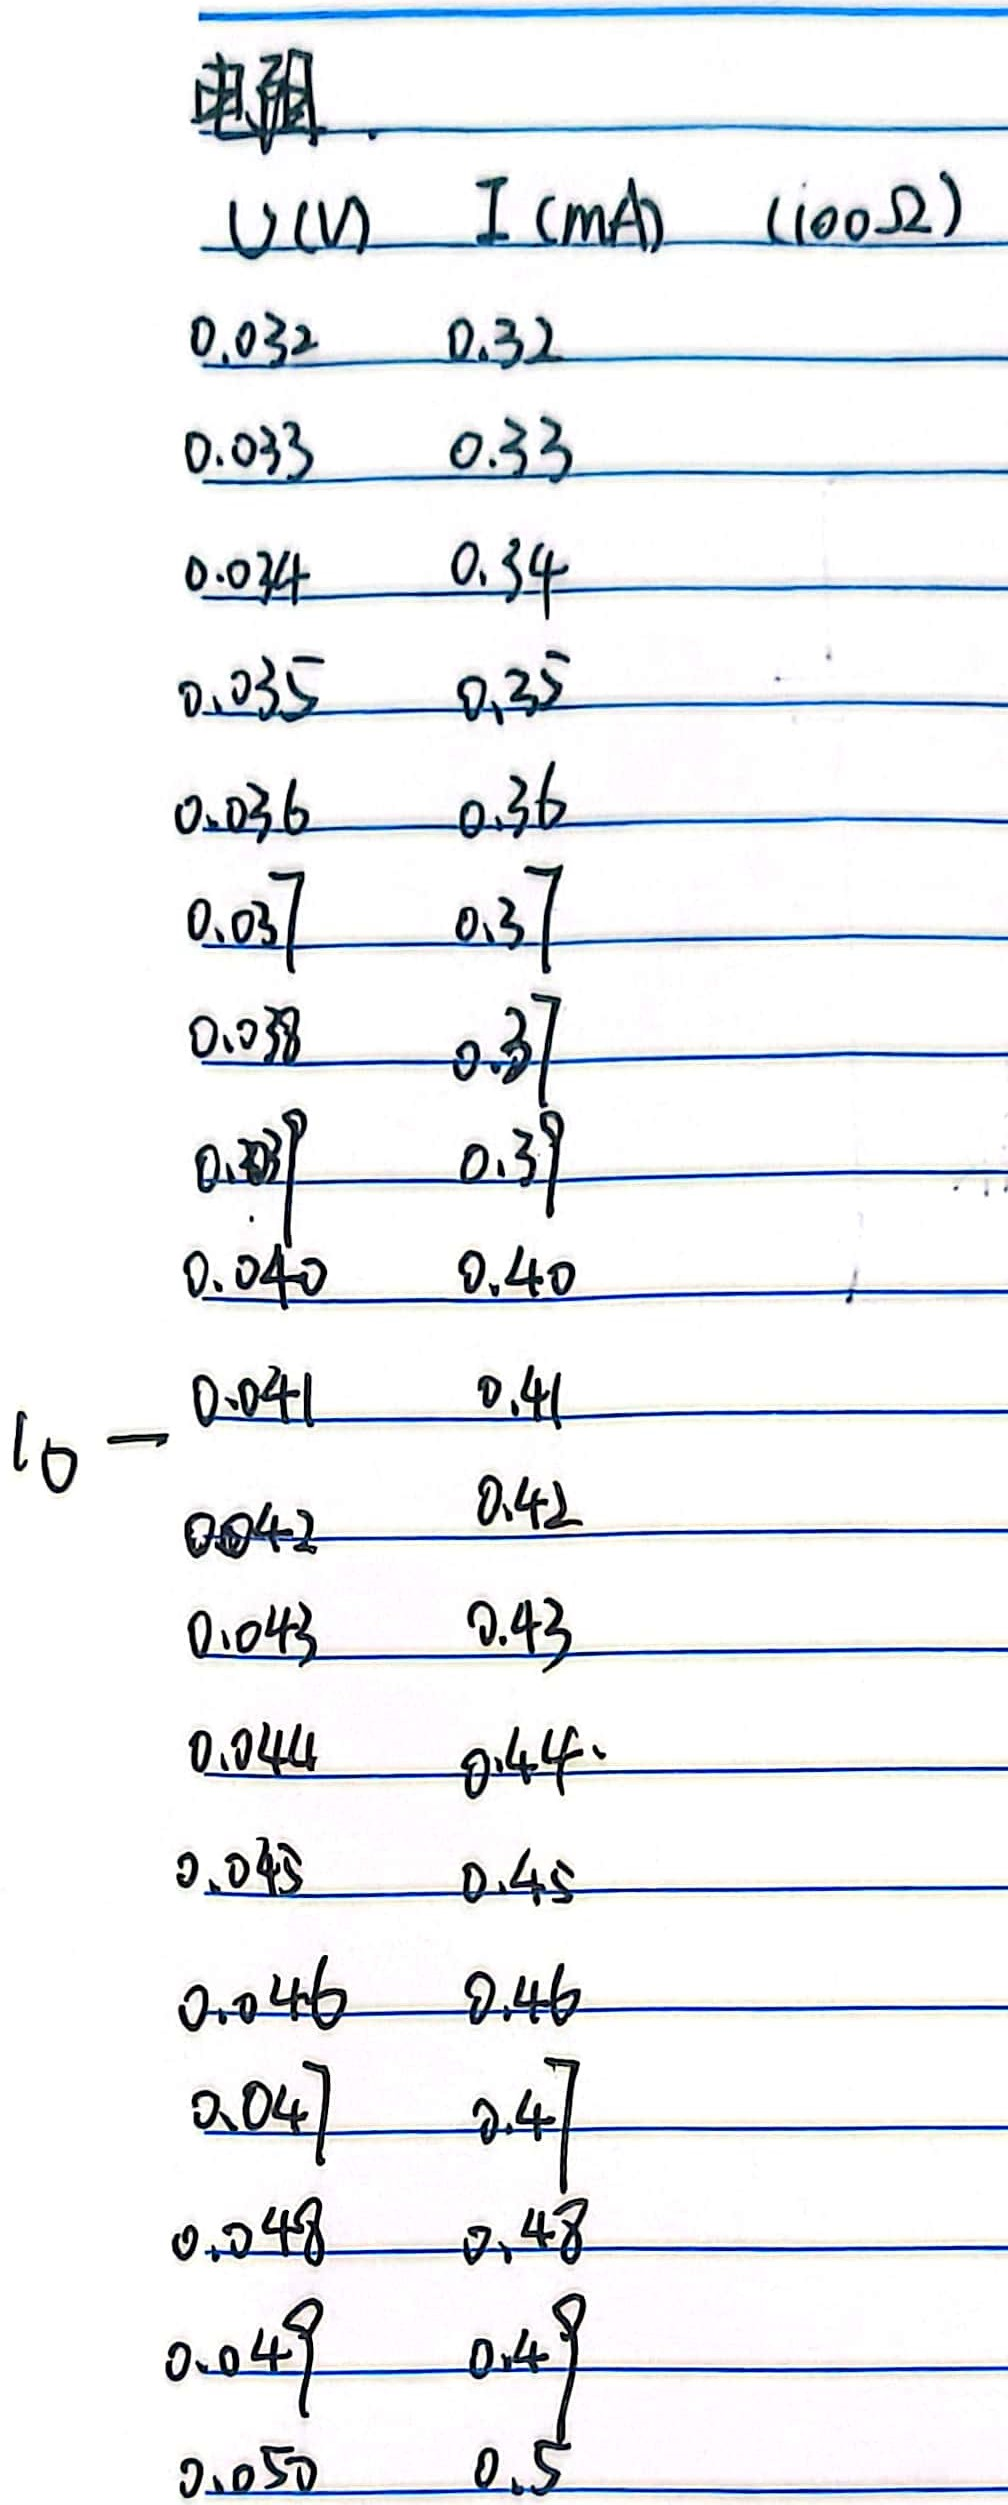
\includegraphics[width=0.9\textwidth,height=0.8\textheight]{dianzu.jpg}
  \caption{实验原始数据1}\label{dianzu}
\end{figure}
\newpage

\begin{figure}[H]
  \centering
  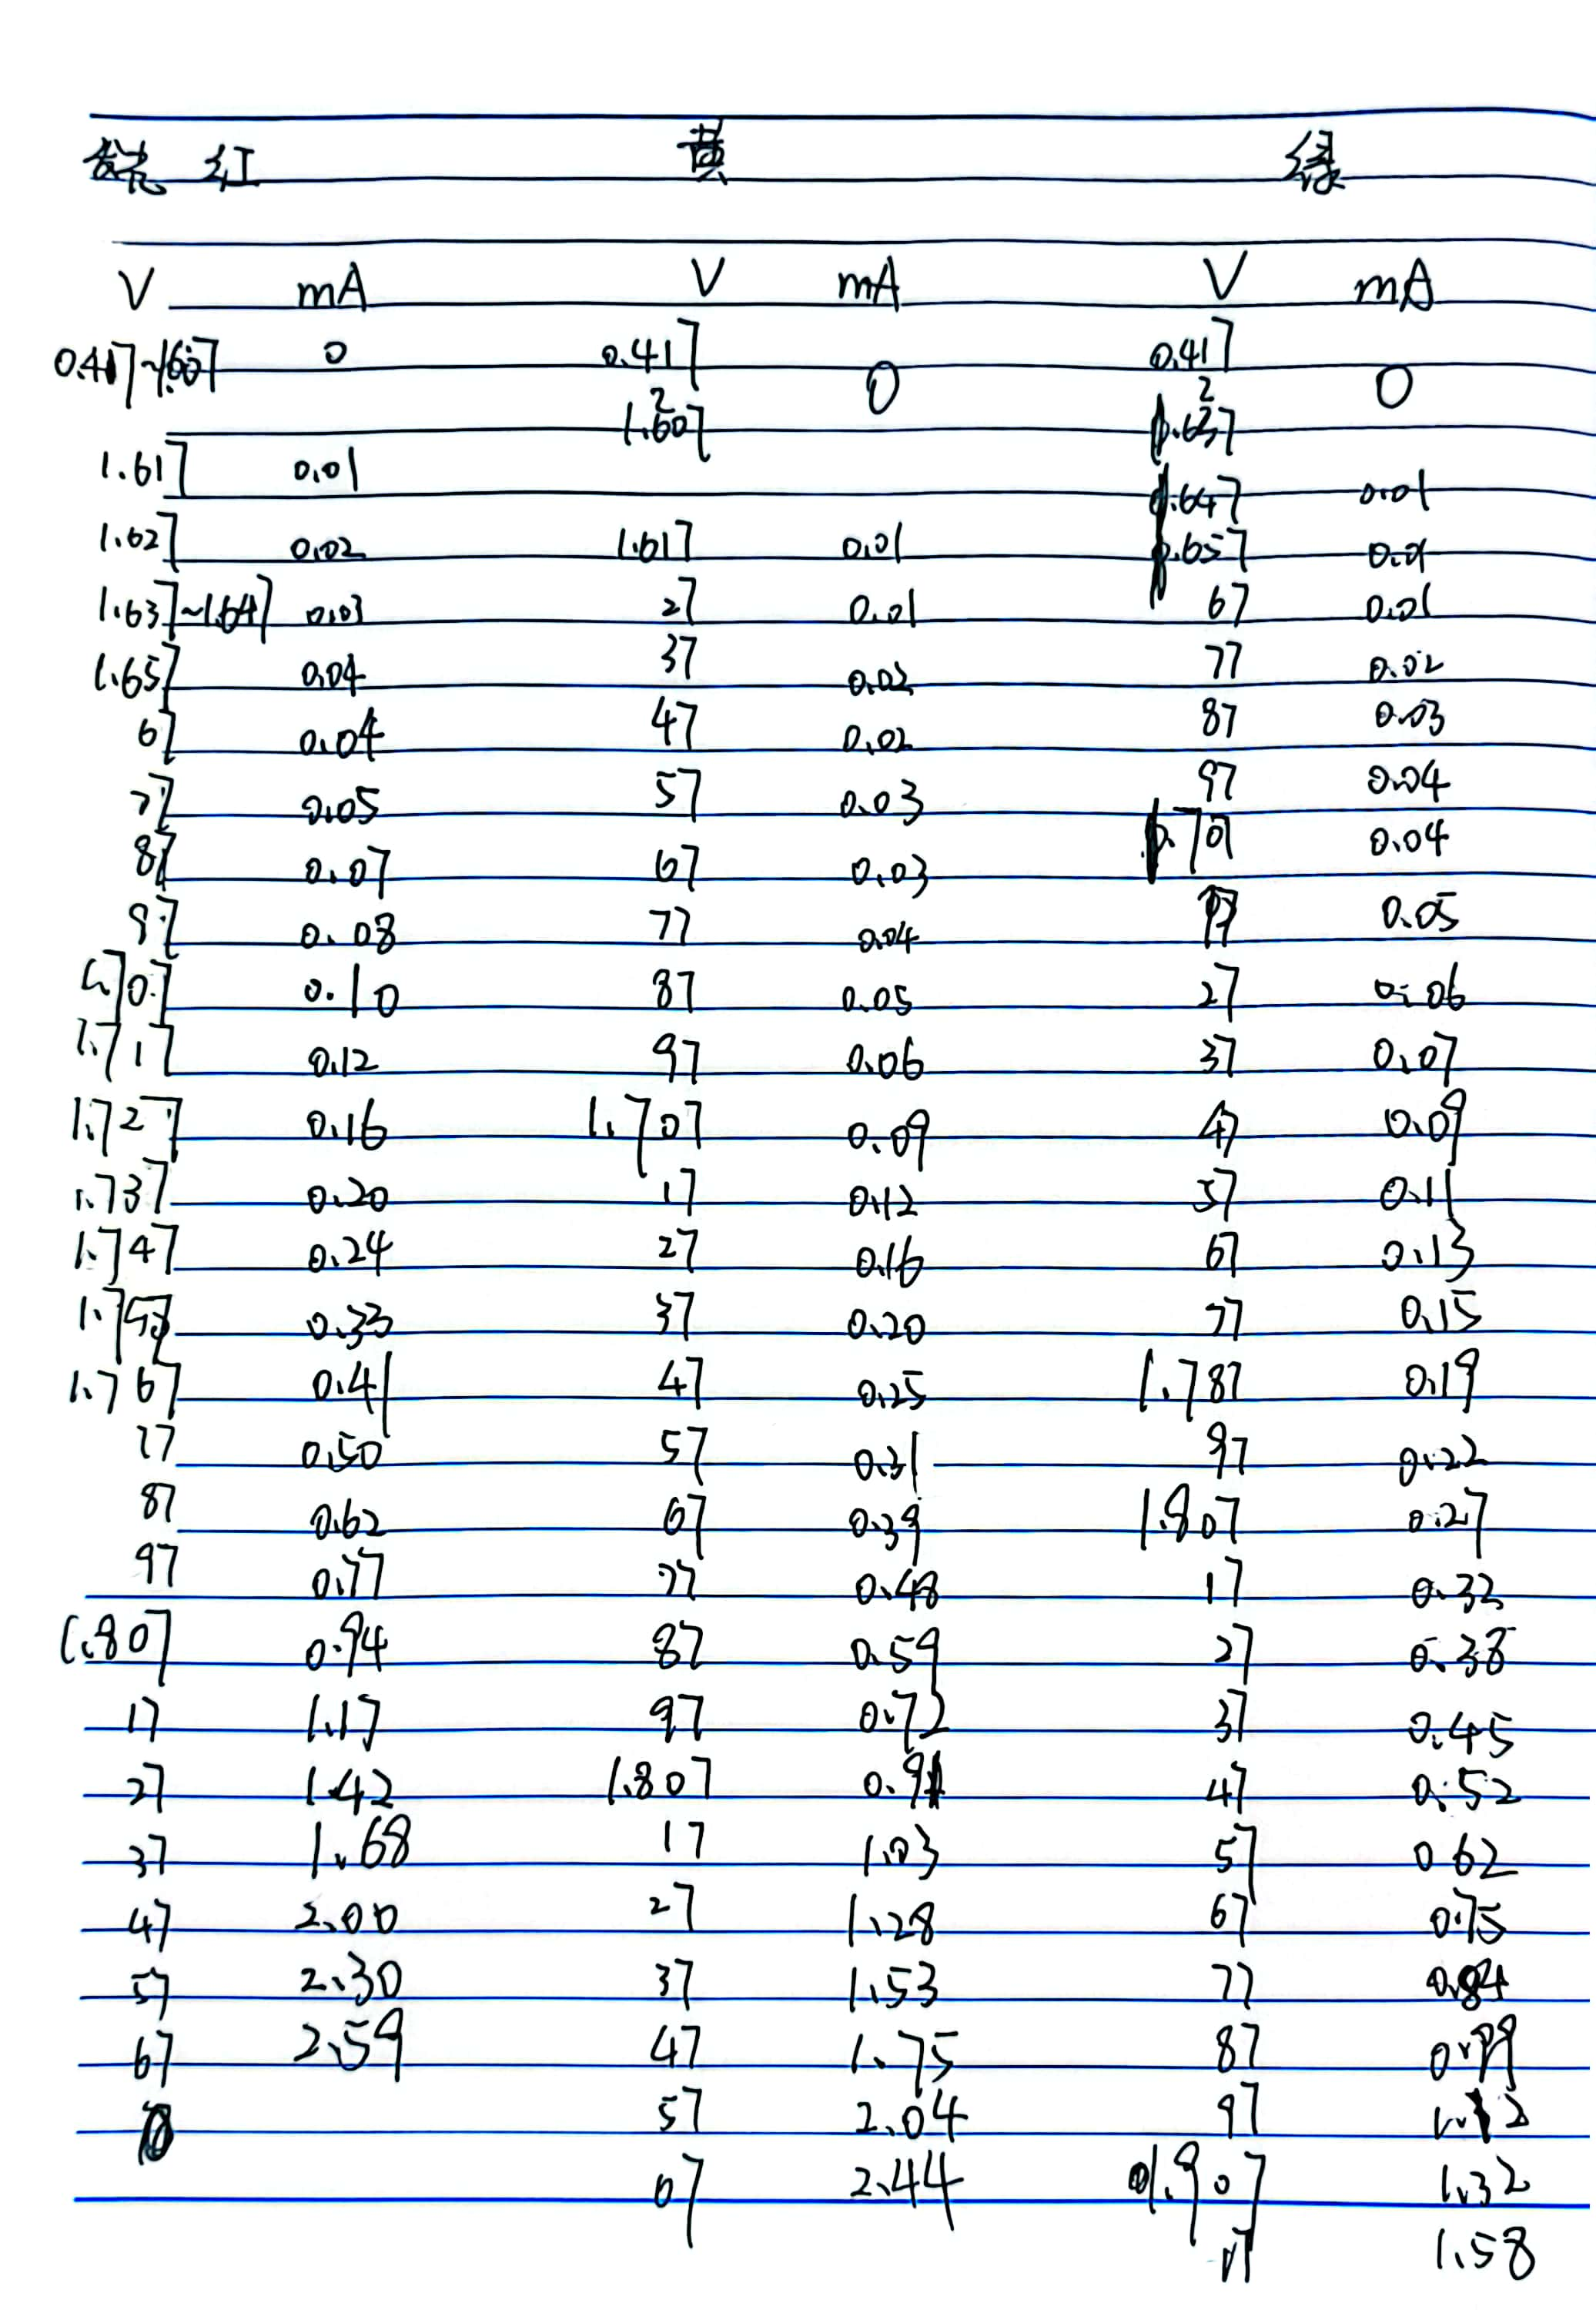
\includegraphics[width=1\textwidth,height=0.8\textheight]{LED1.jpg}
  \caption{实验原始数据2}\label{LED1}
\end{figure}
\newpage

\begin{figure}[H]
  \centering
  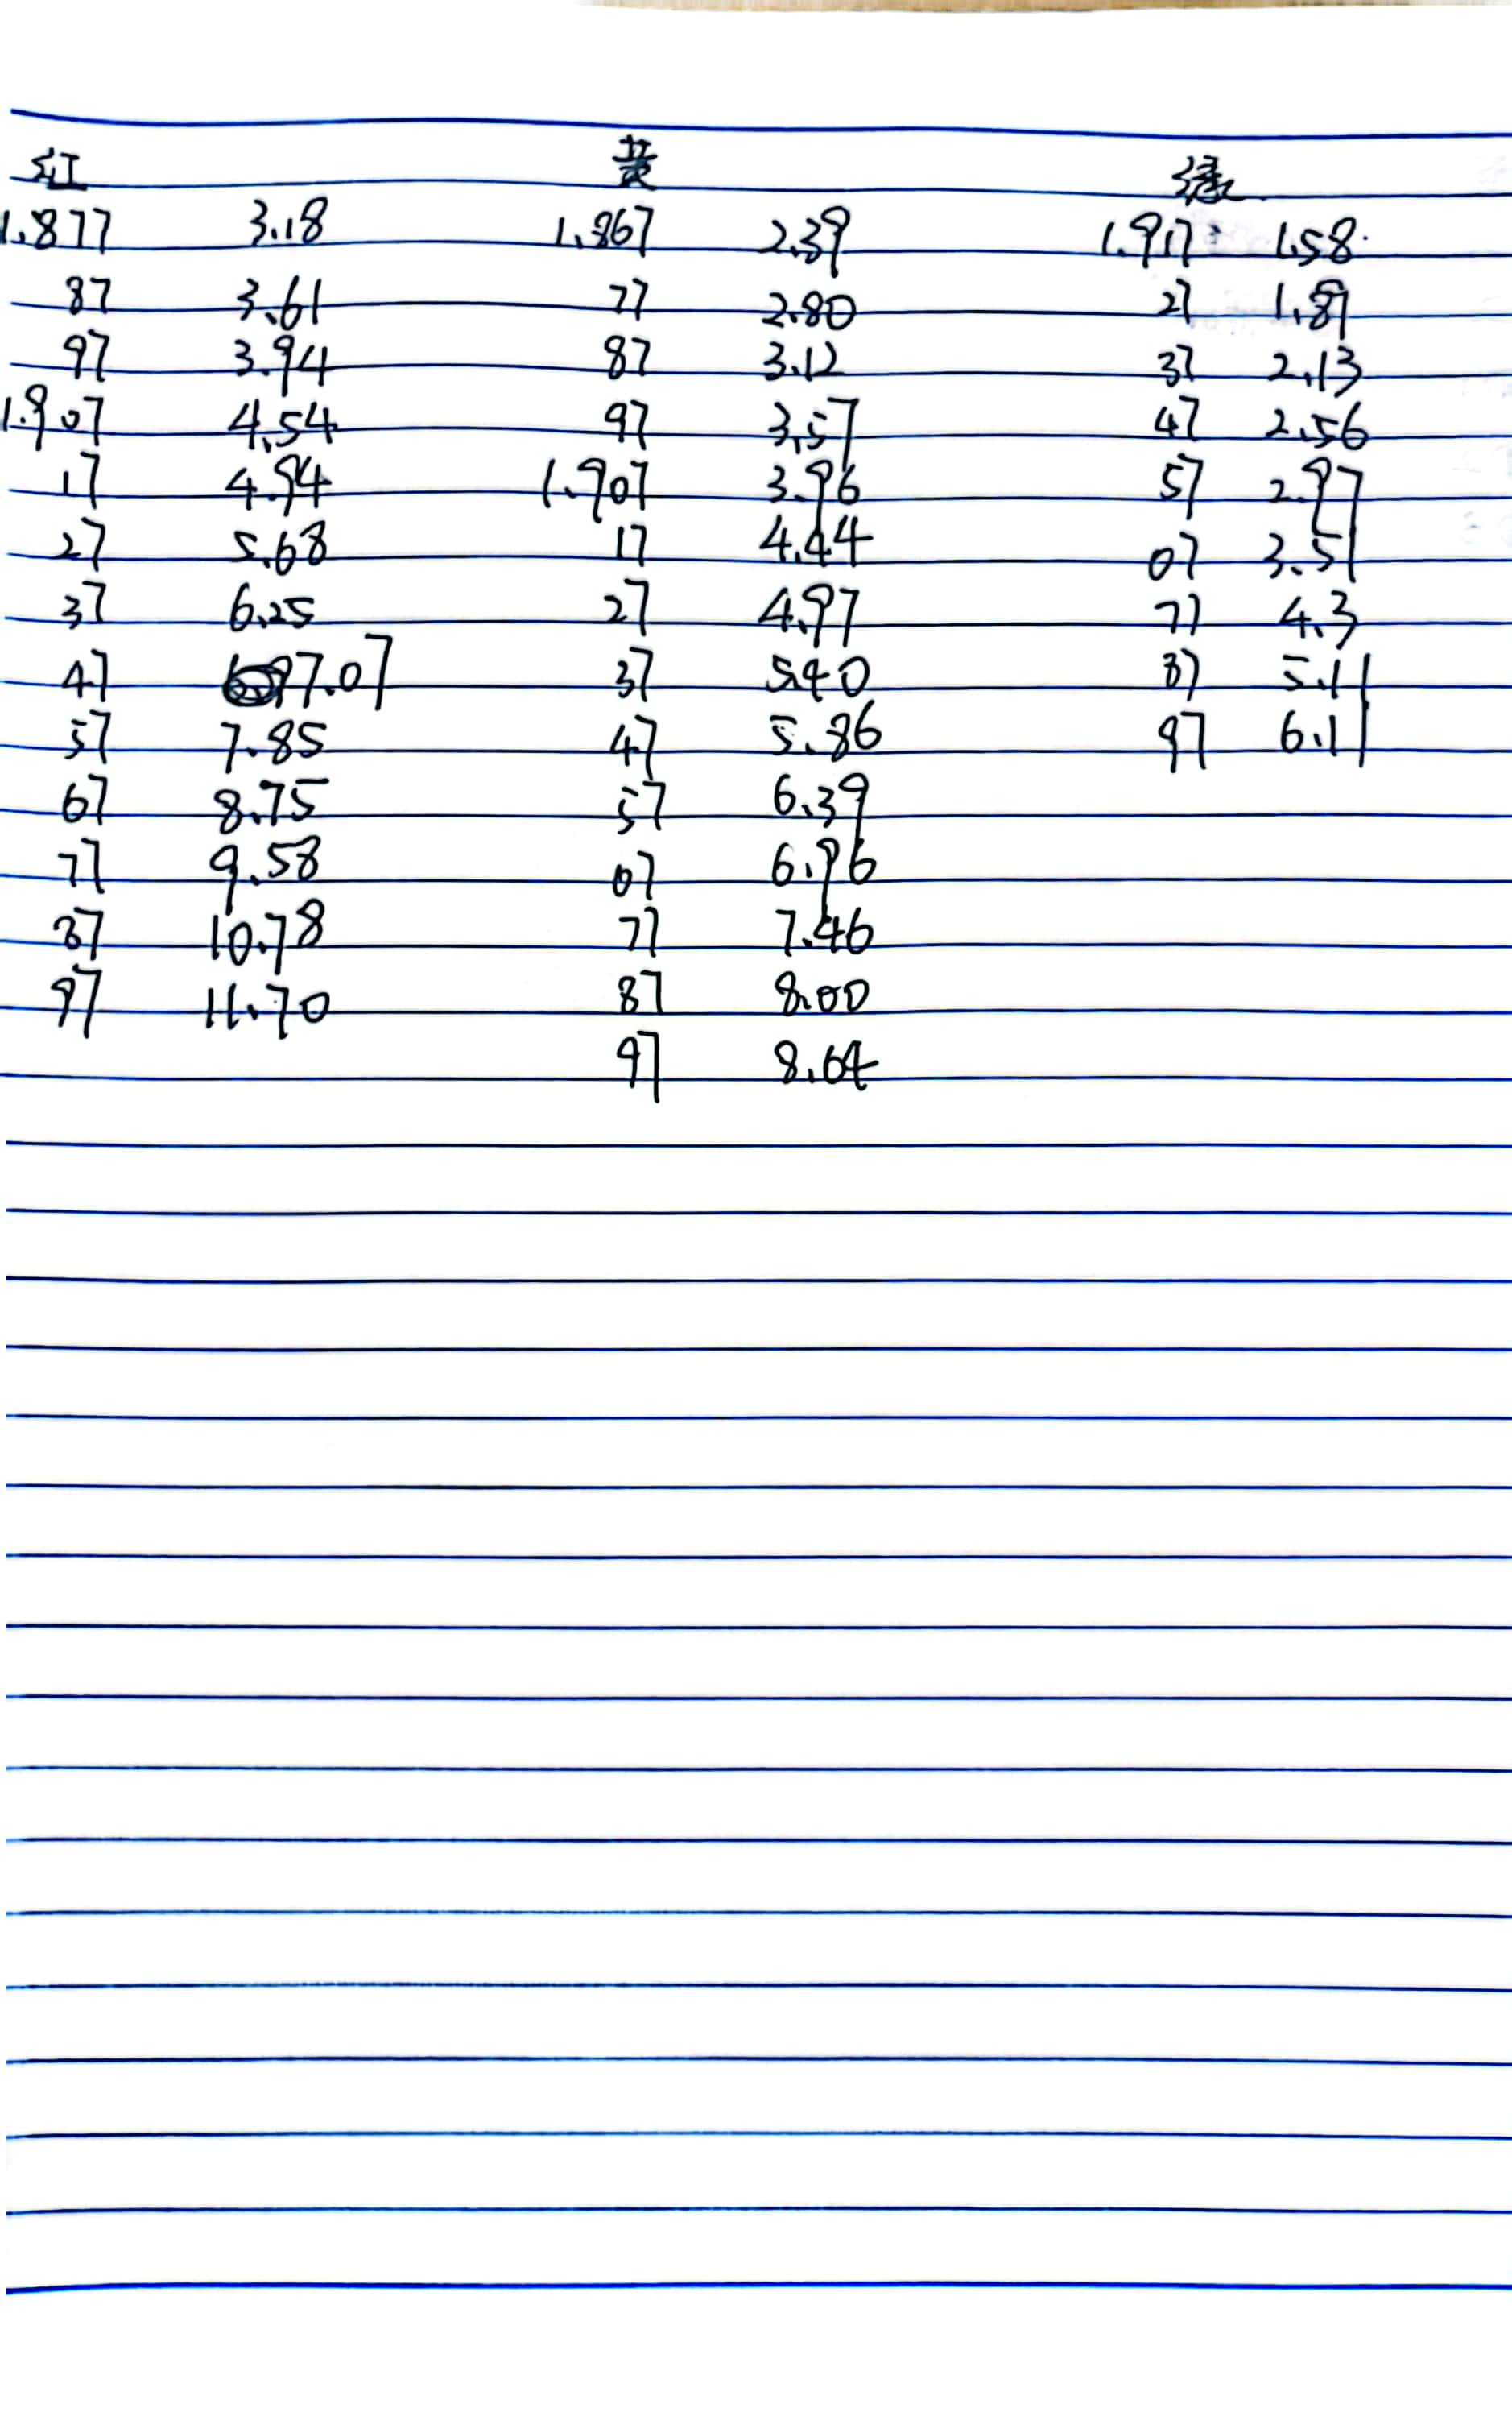
\includegraphics[width=1\textwidth,height=0.8\textheight]{LED2.jpg}
  \caption{实验原始数据3}\label{LED2}
\end{figure}
\newpage

\begin{figure}[H]
  \centering
  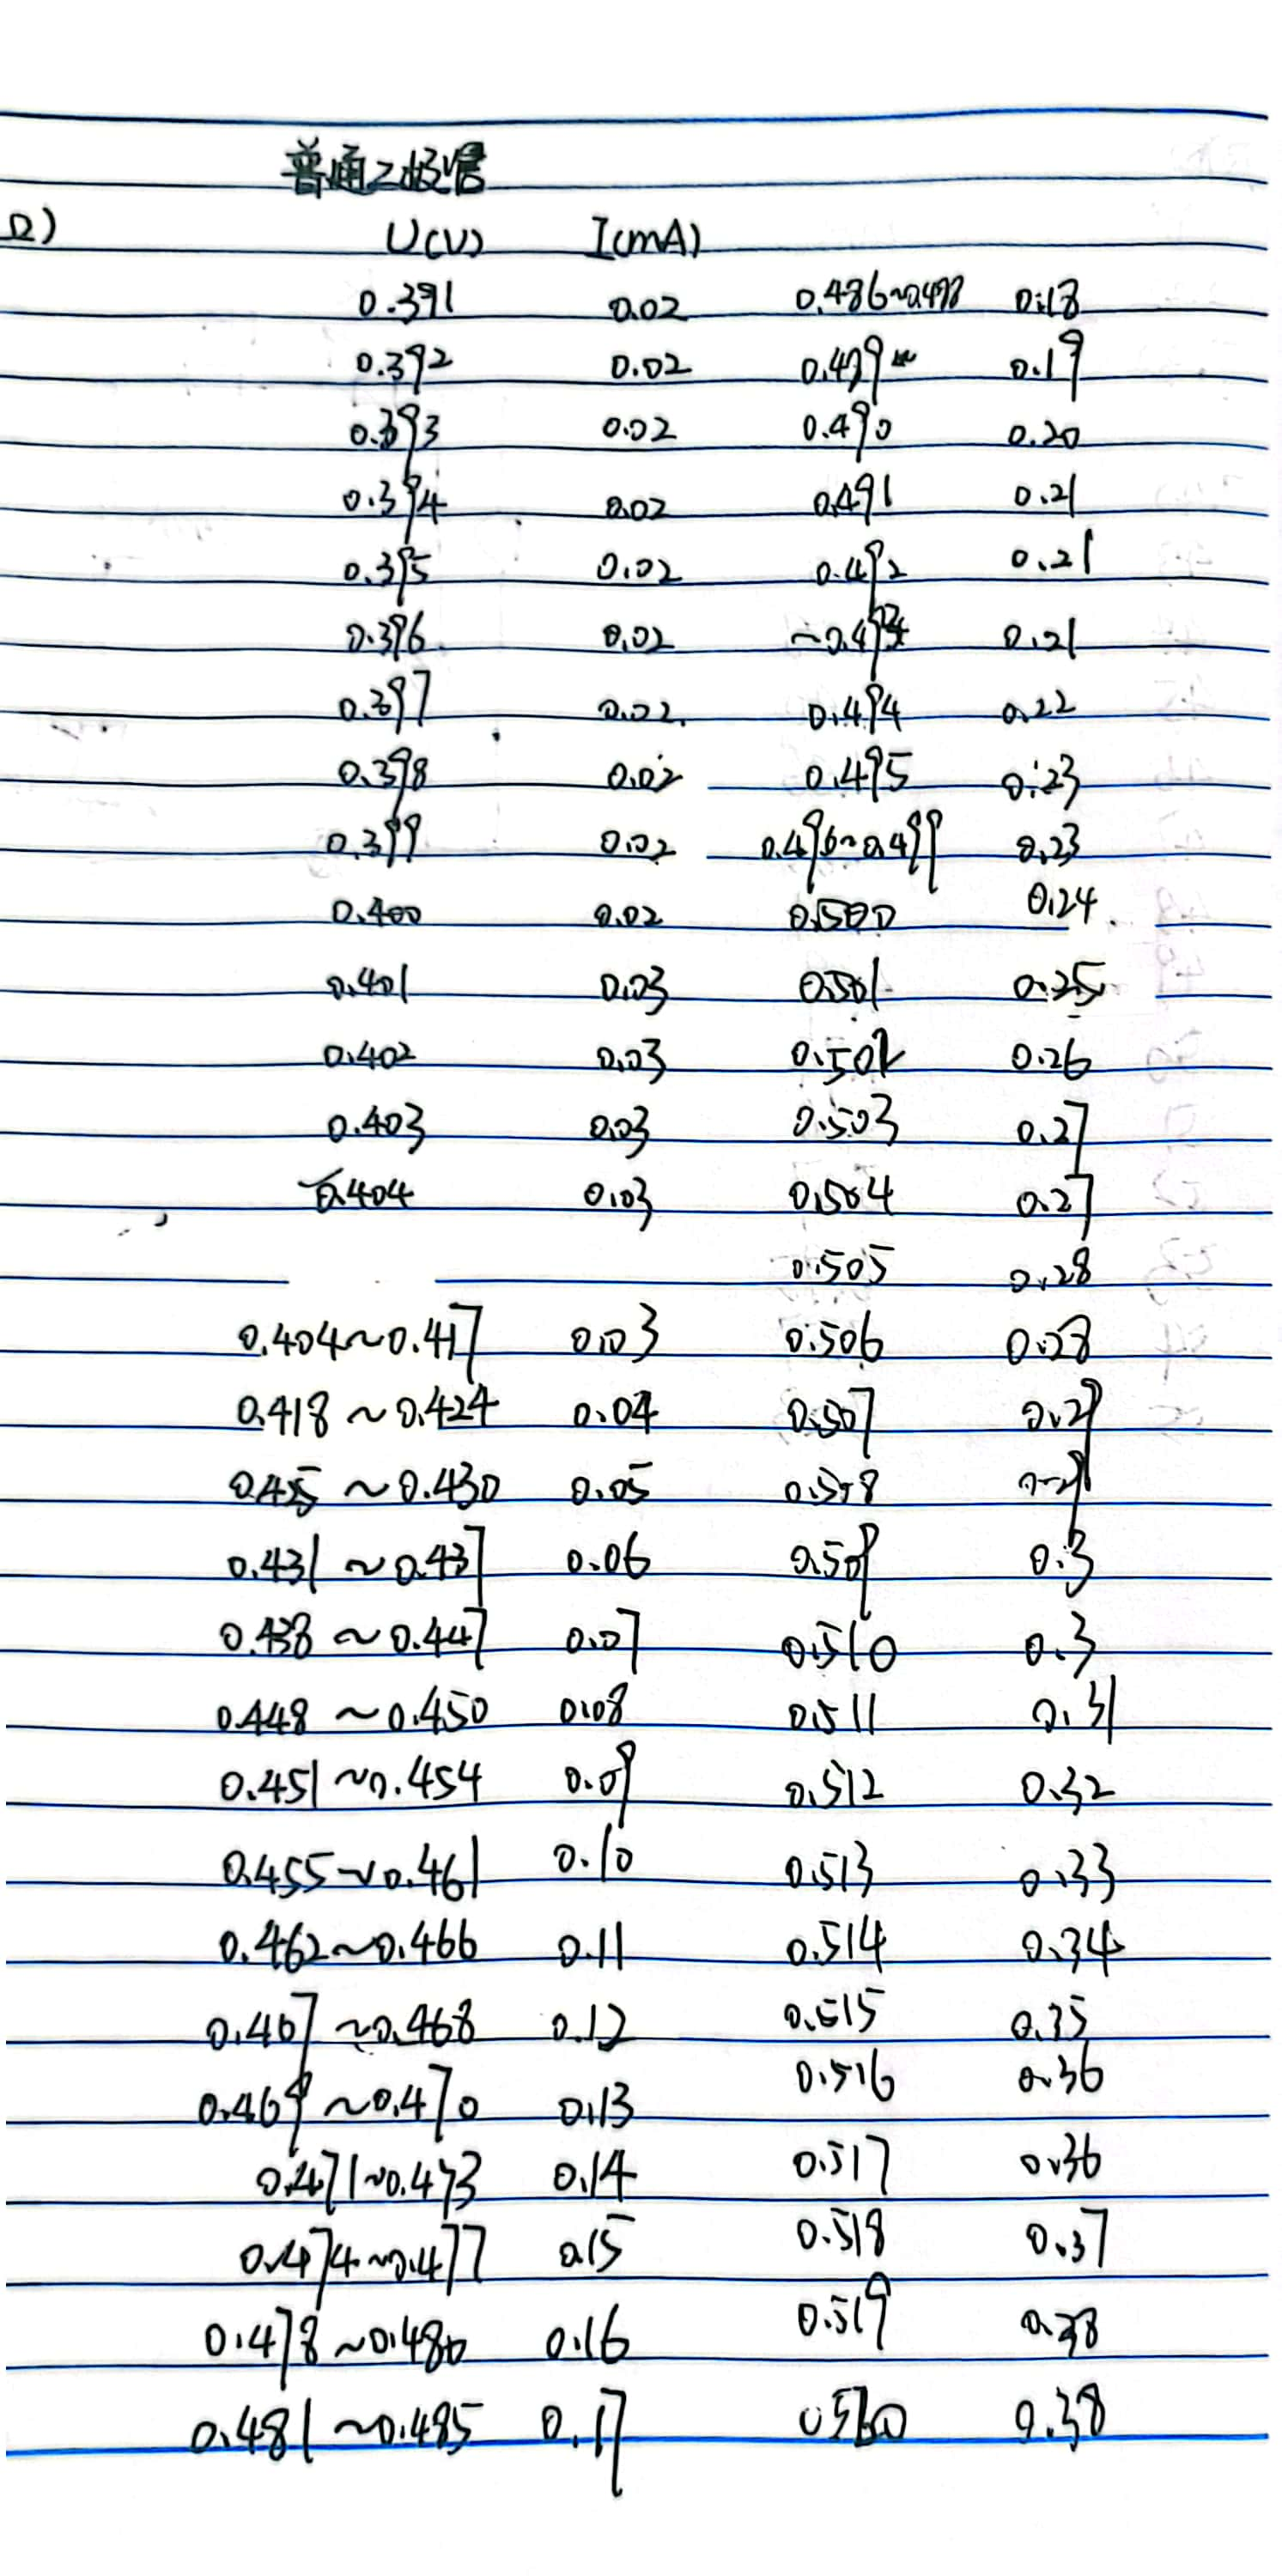
\includegraphics[width=1\textwidth,height=0.8\textheight]{putong1.jpg}
  \caption{实验原始数据4}\label{putong1}
\end{figure}
\newpage

\begin{figure}[H]
  \centering
  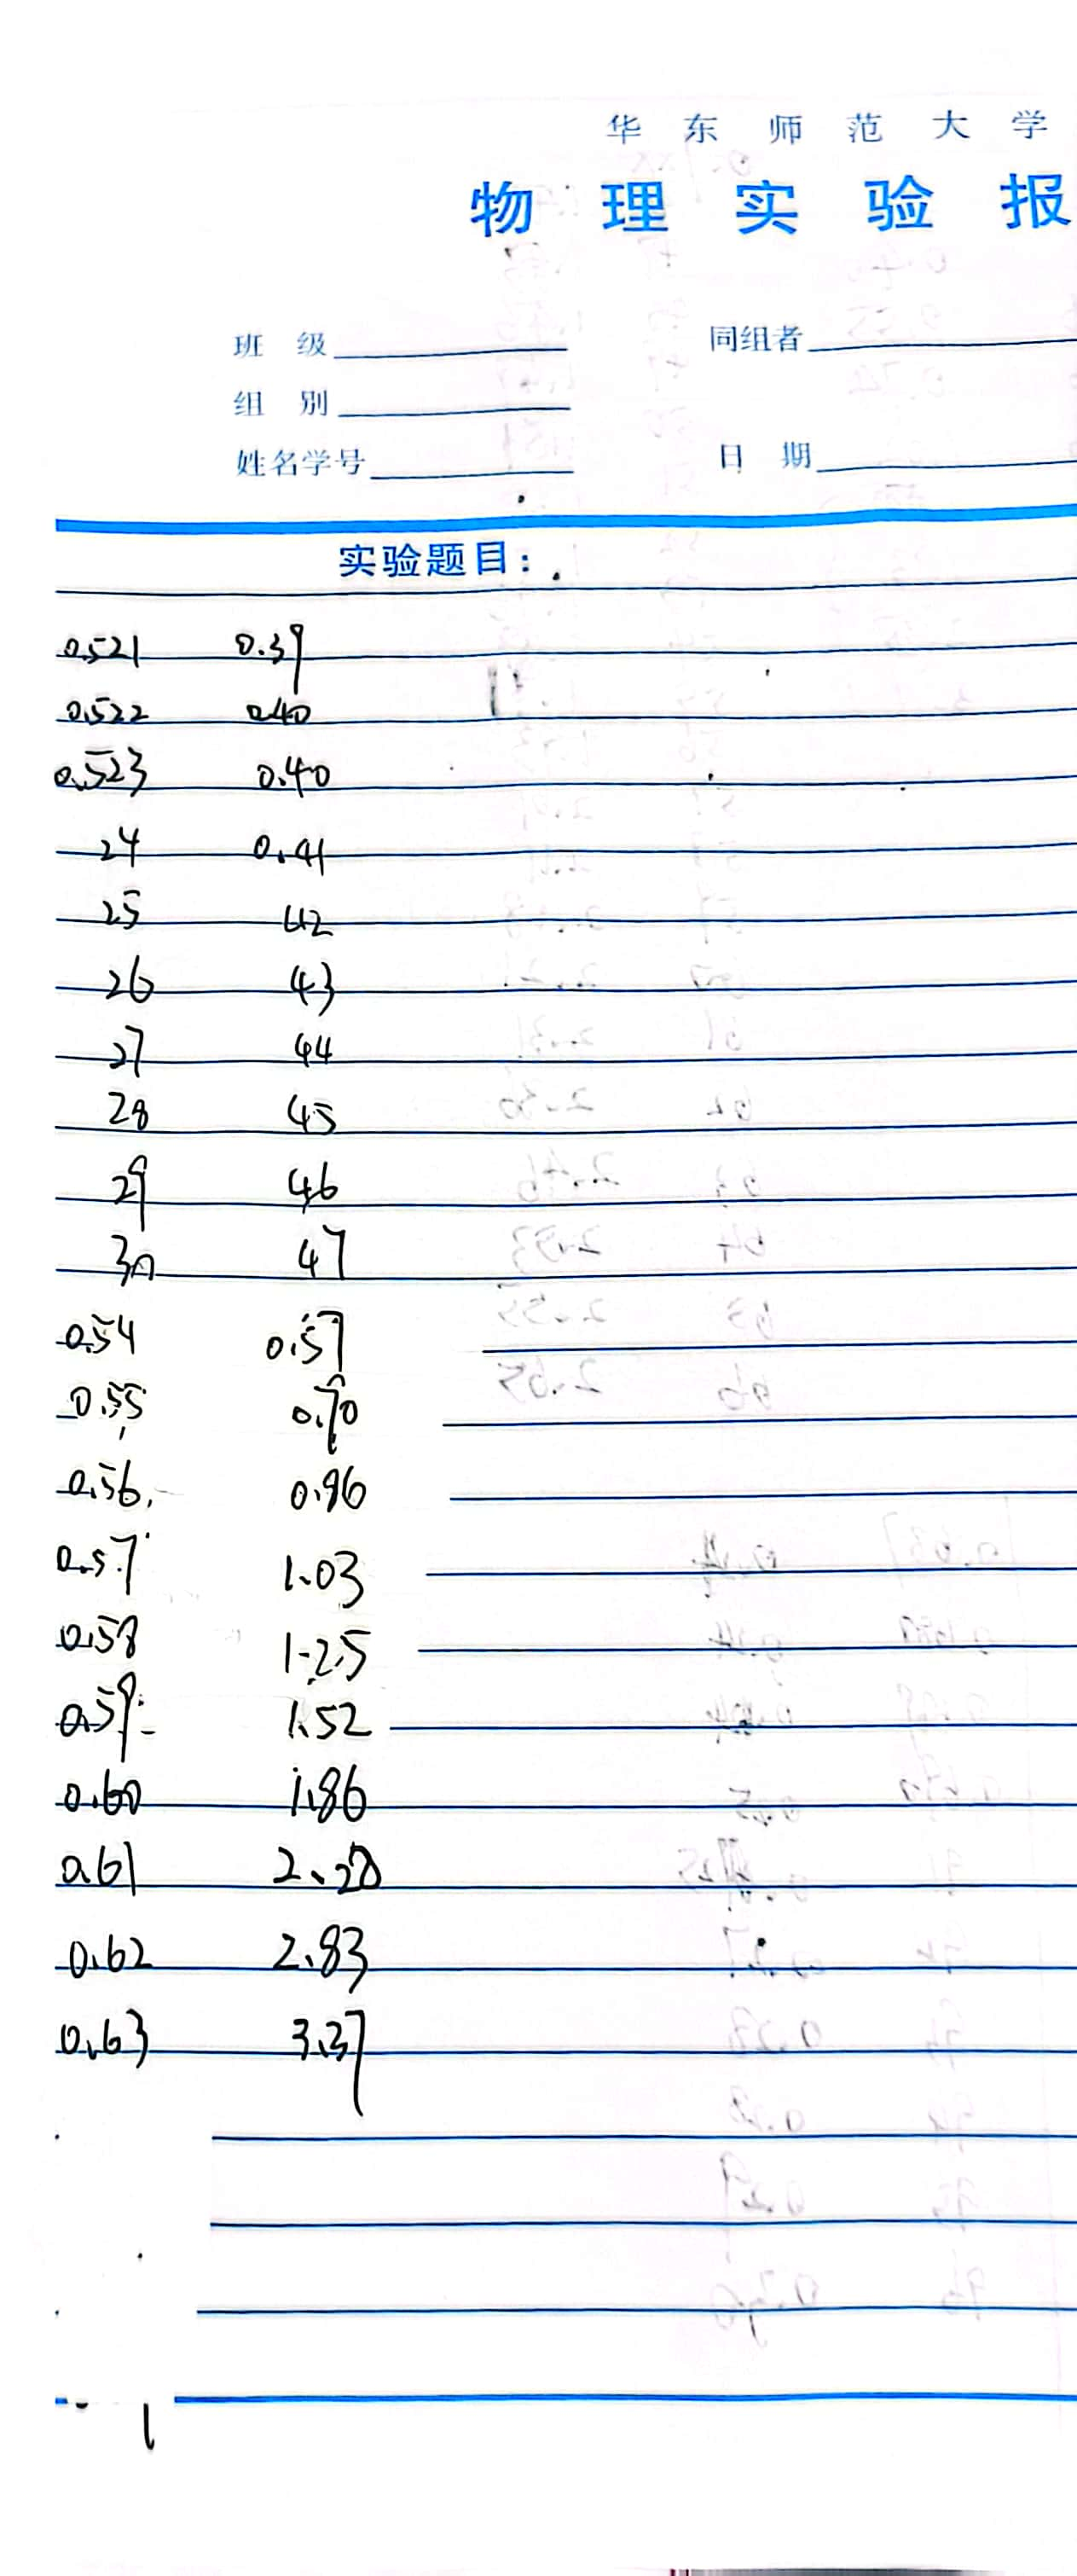
\includegraphics[width=1\textwidth,height=0.8\textheight]{putong2.jpg}
  \caption{实验原始数据5}\label{putong2}
\end{figure}
\newpage

\begin{figure}[H]
  \centering
  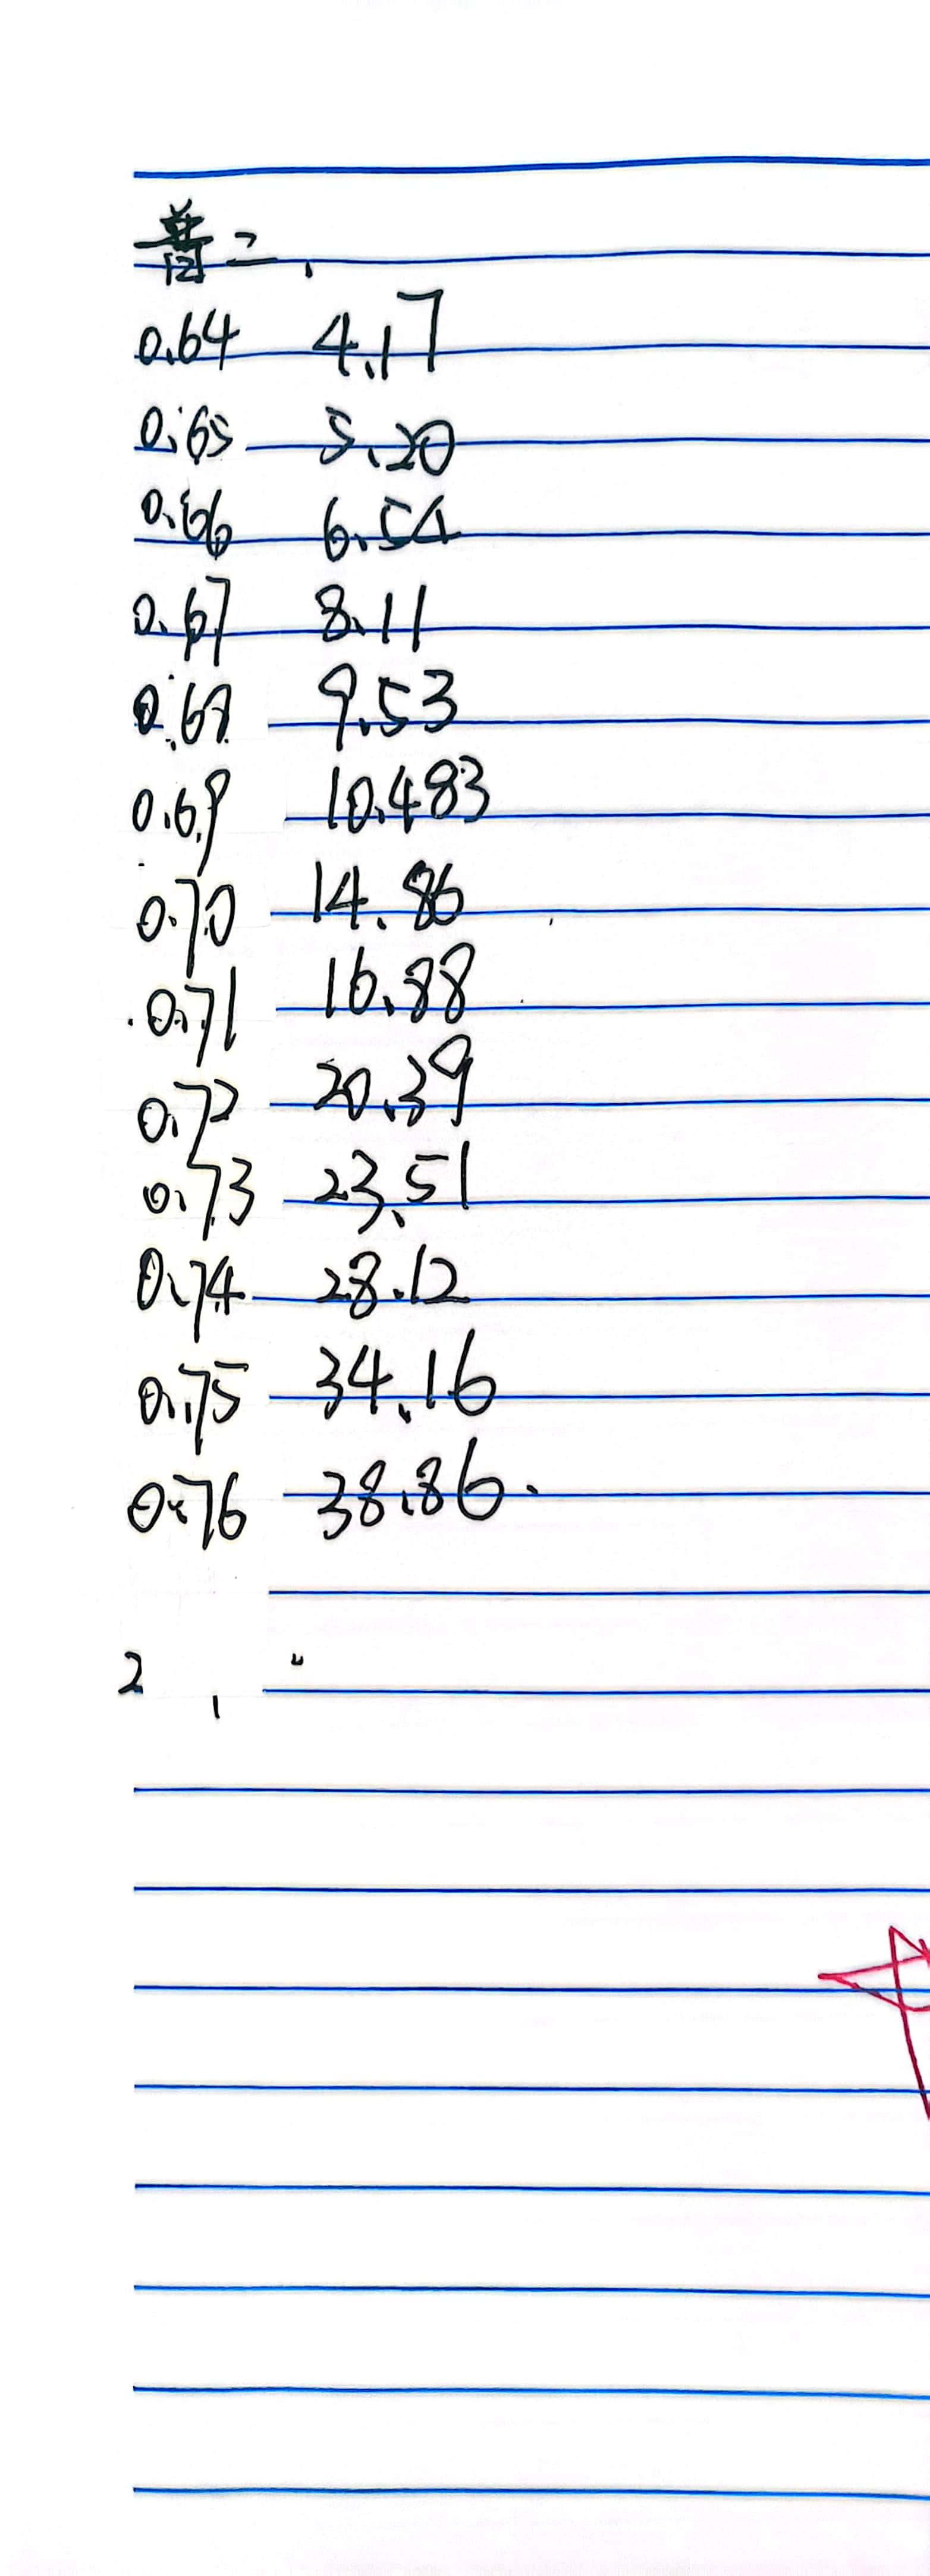
\includegraphics[width=1\textwidth,height=0.8\textheight]{putong3.jpg}
  \caption{实验原始数据6}\label{putong3}
\end{figure}
\newpage

\begin{figure}[H]
  \centering
  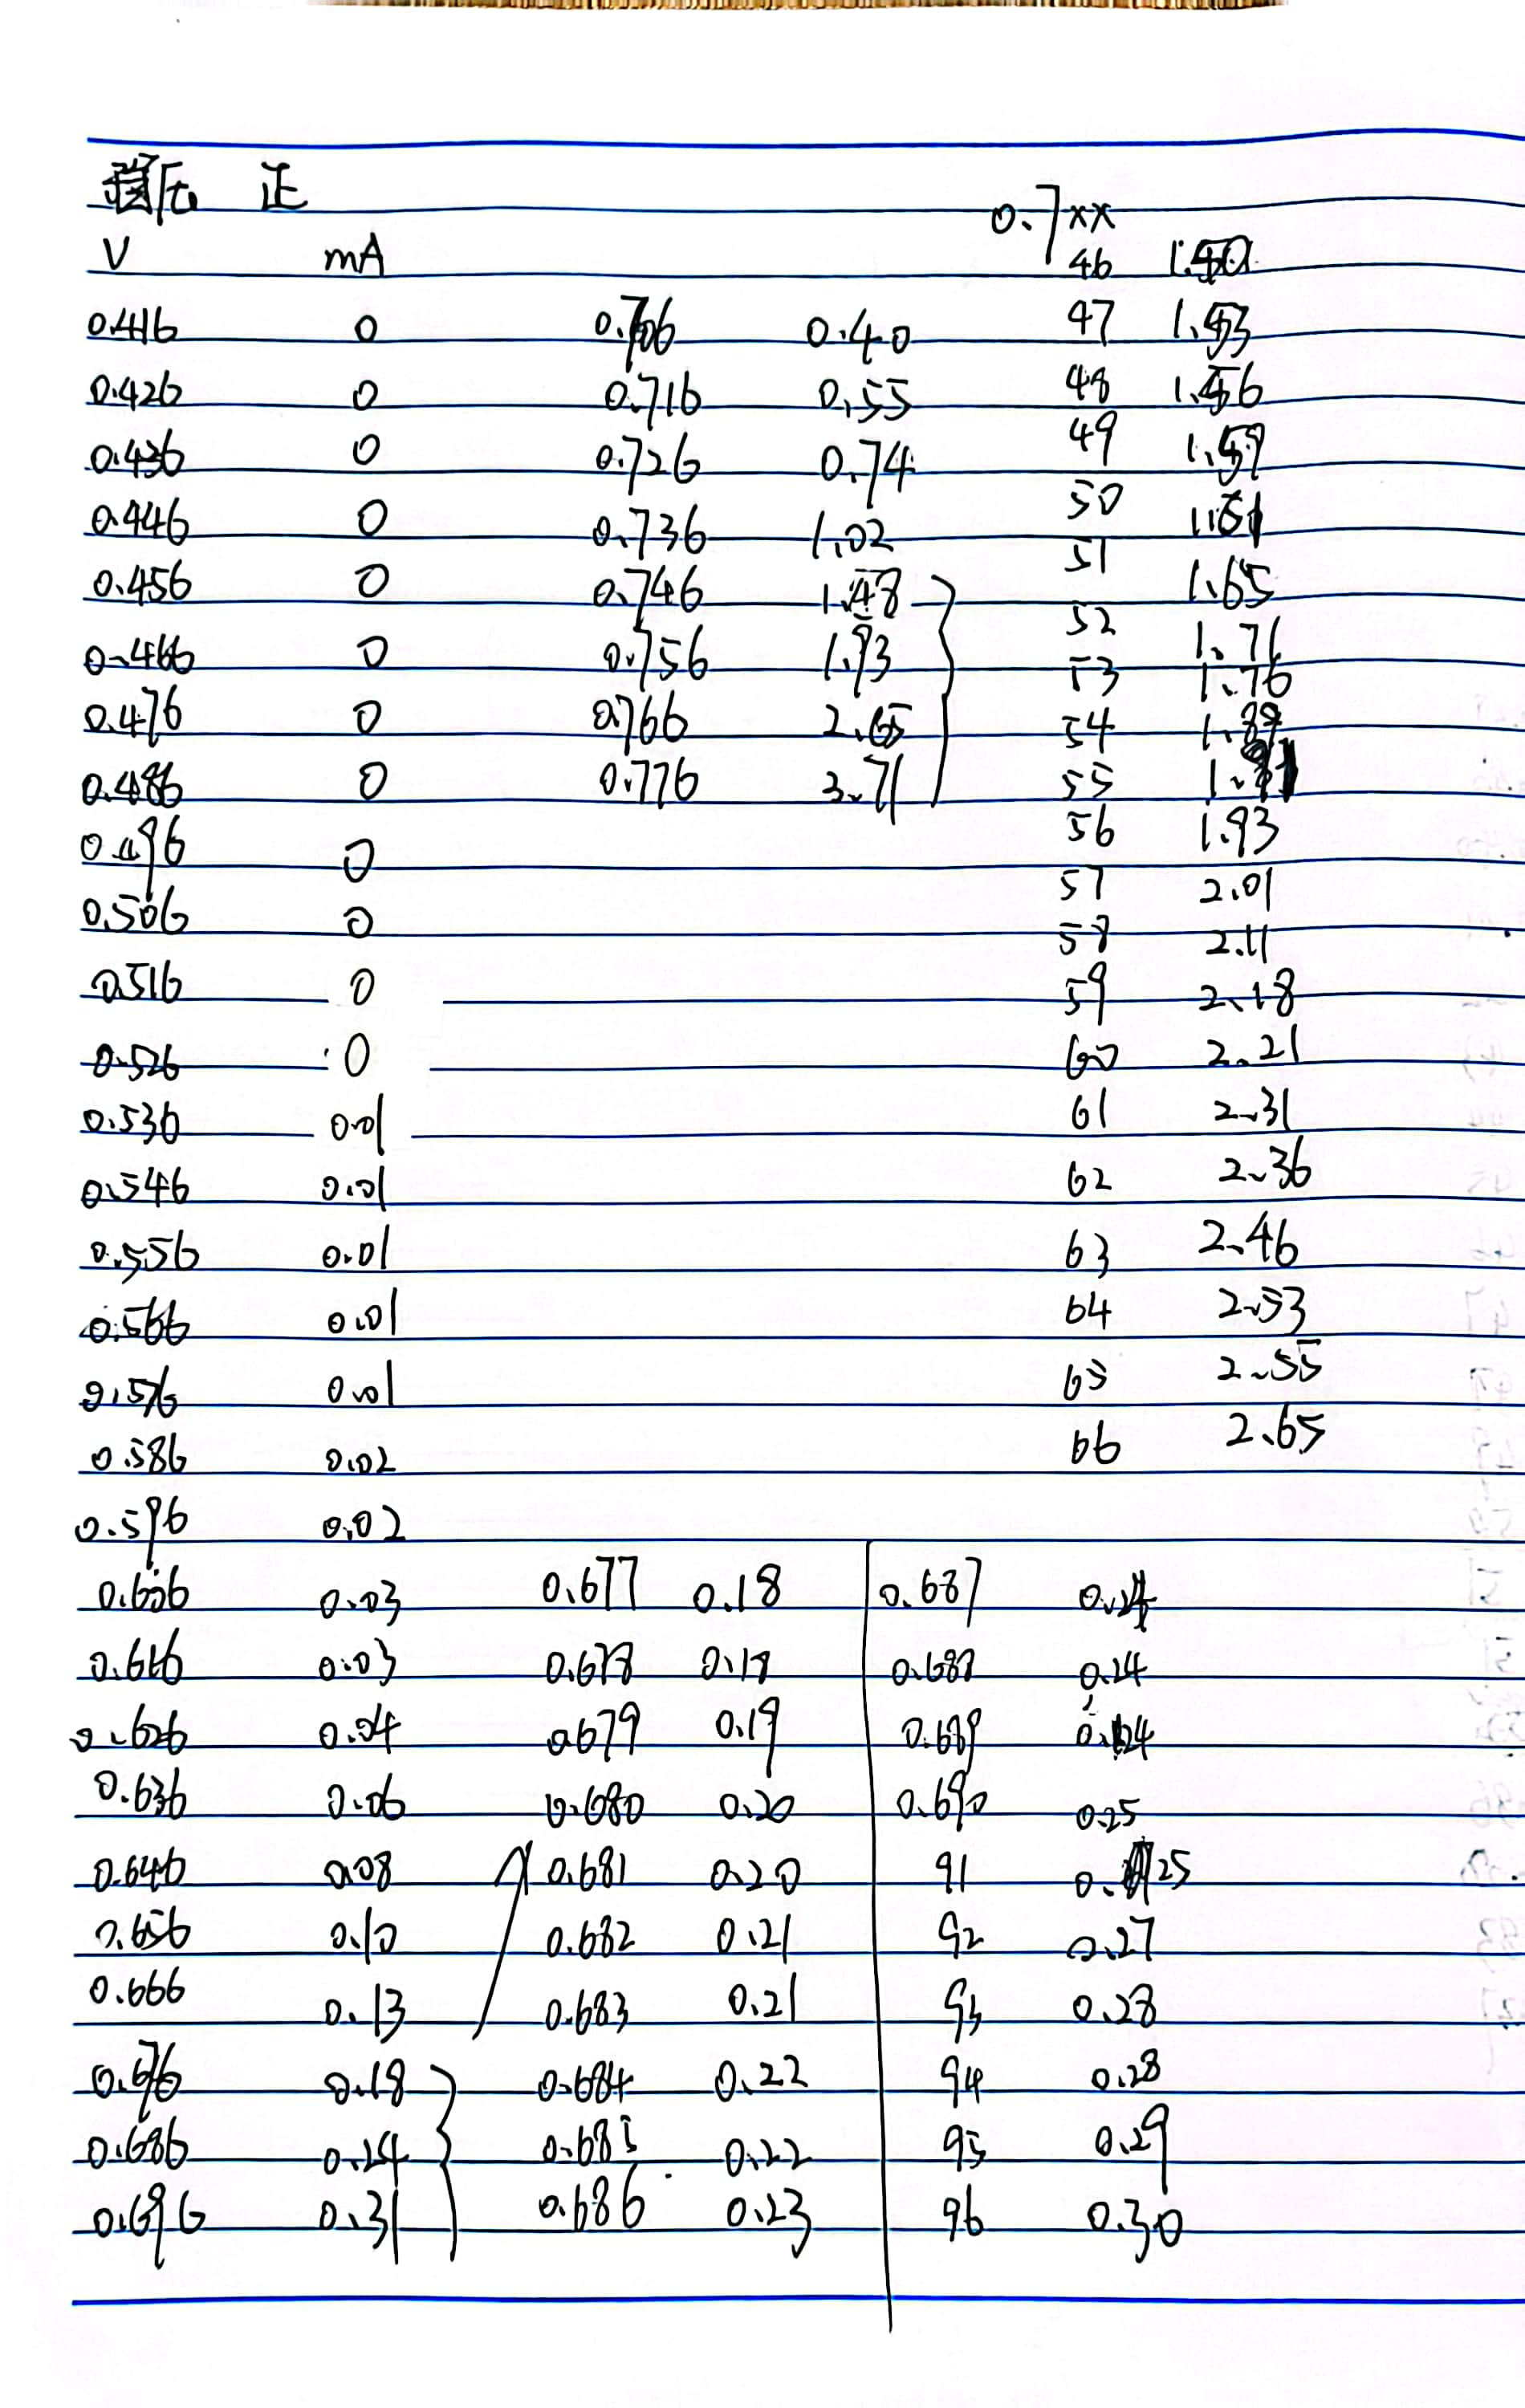
\includegraphics[width=1\textwidth,height=0.8\textheight]{wenyazhengxiang1.jpg}
  \caption{实验原始数据7}\label{wenyazhengxiang1}
\end{figure}
\newpage

\begin{figure}[H]
  \centering
  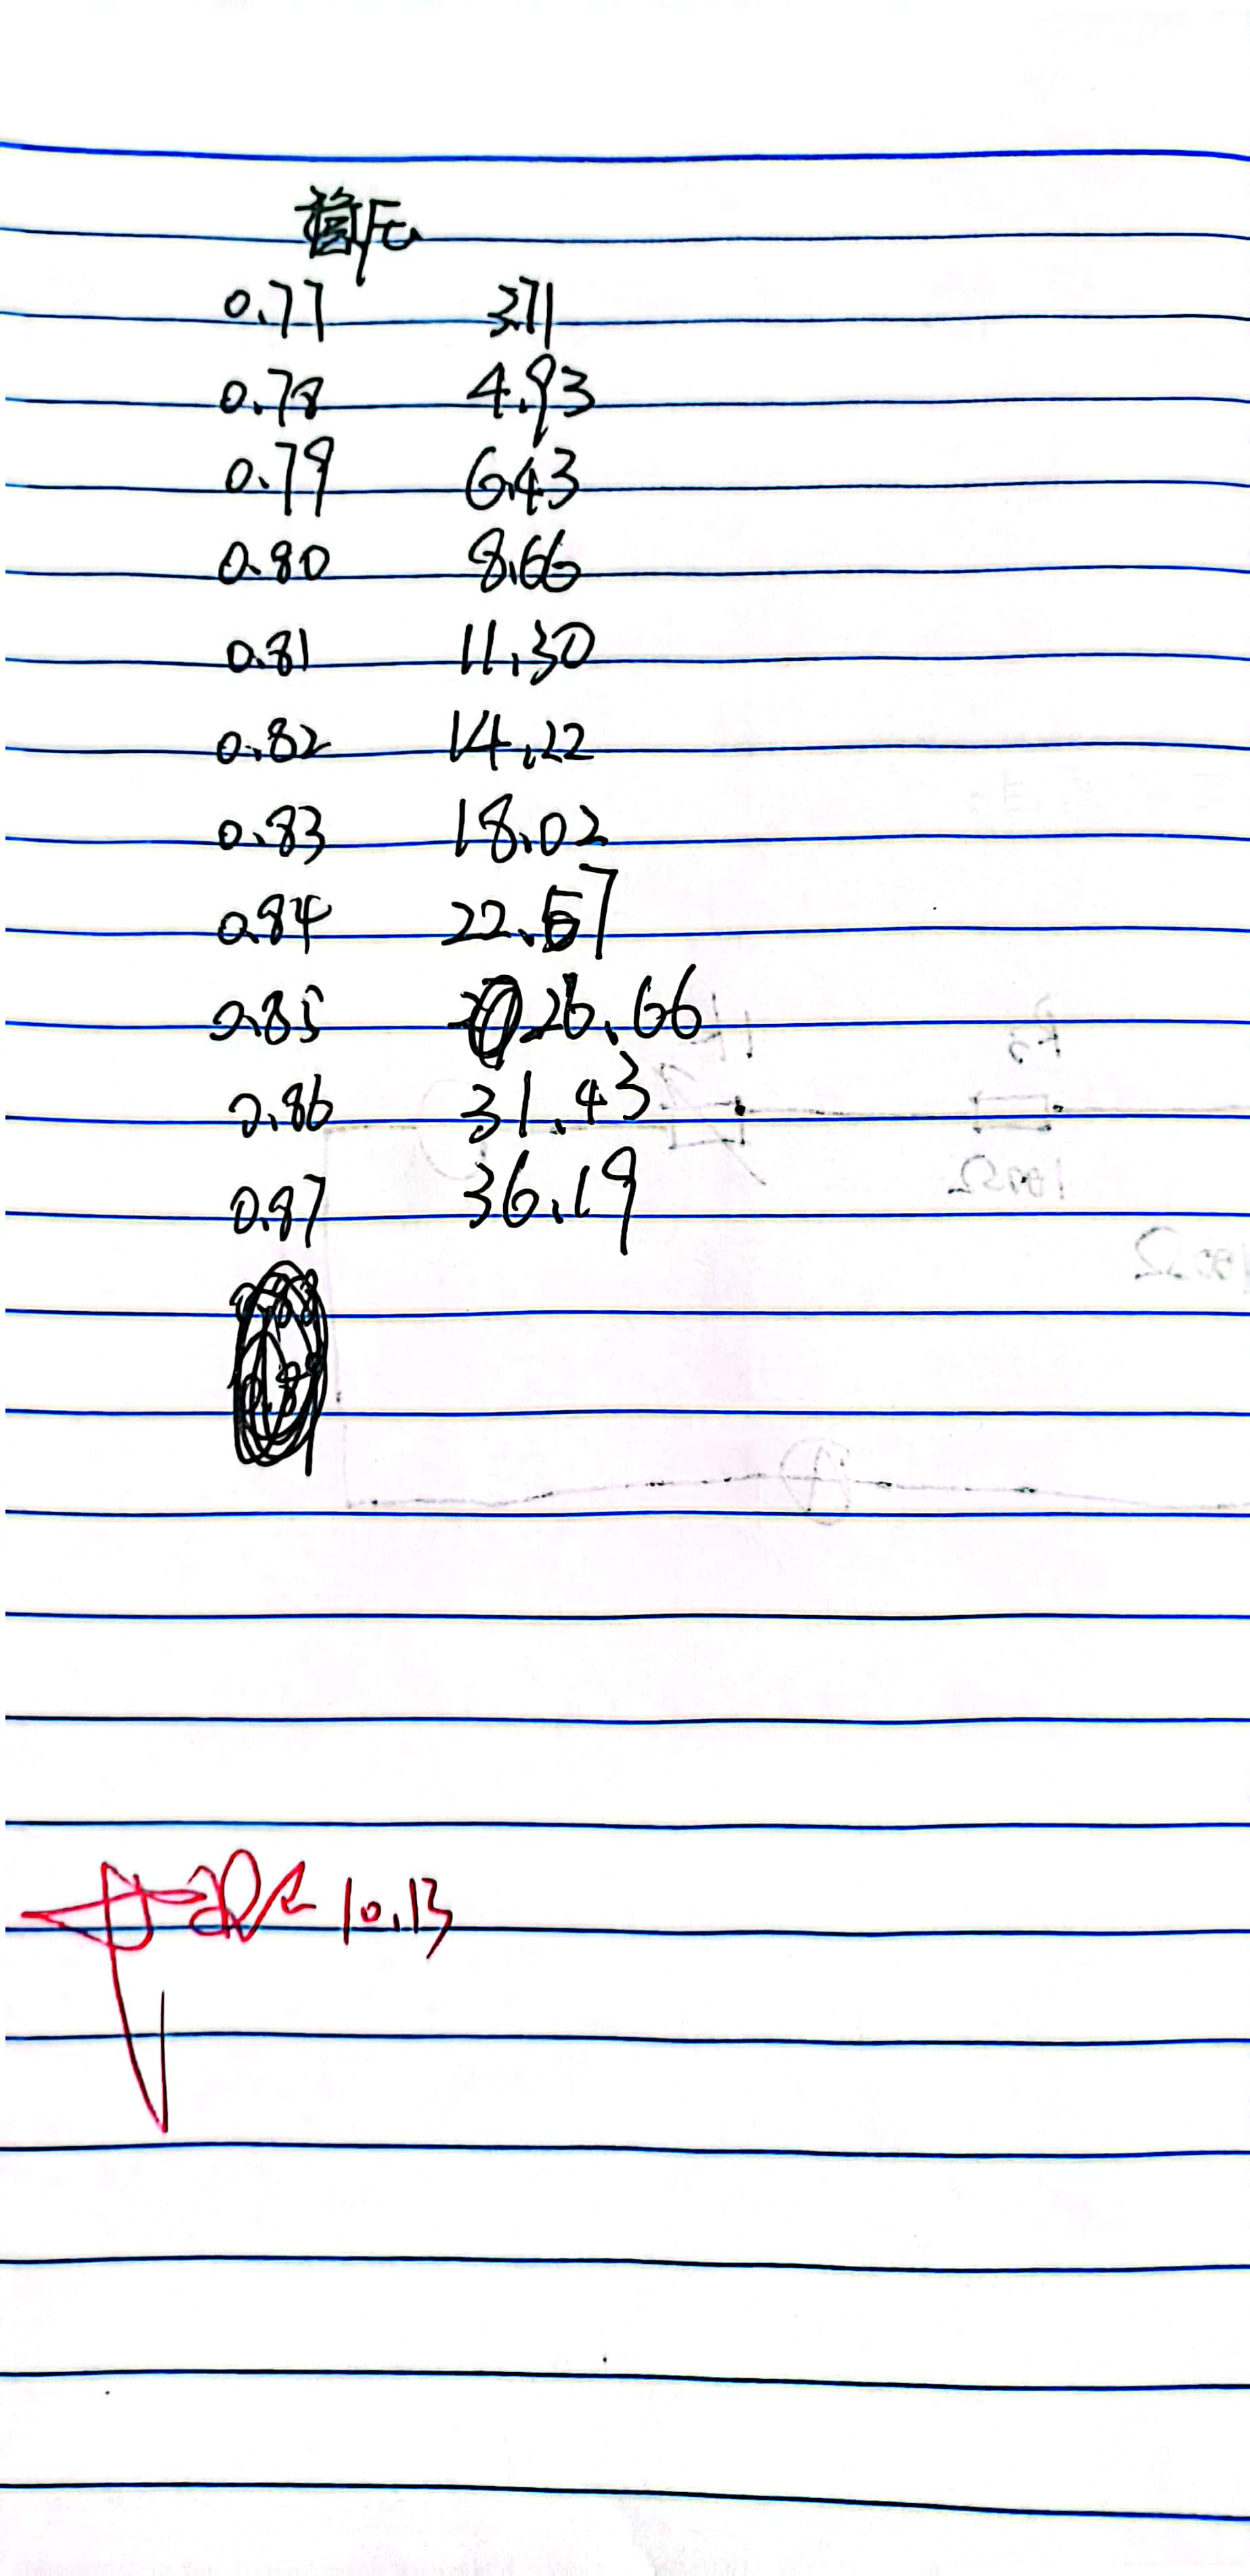
\includegraphics[width=1\textwidth,height=0.8\textheight]{wenyazhengxiang2.jpg}
  \caption{实验原始数据8}\label{wenyazhengxiang2}
\end{figure}
\newpage

\begin{figure}[H]
  \centering
  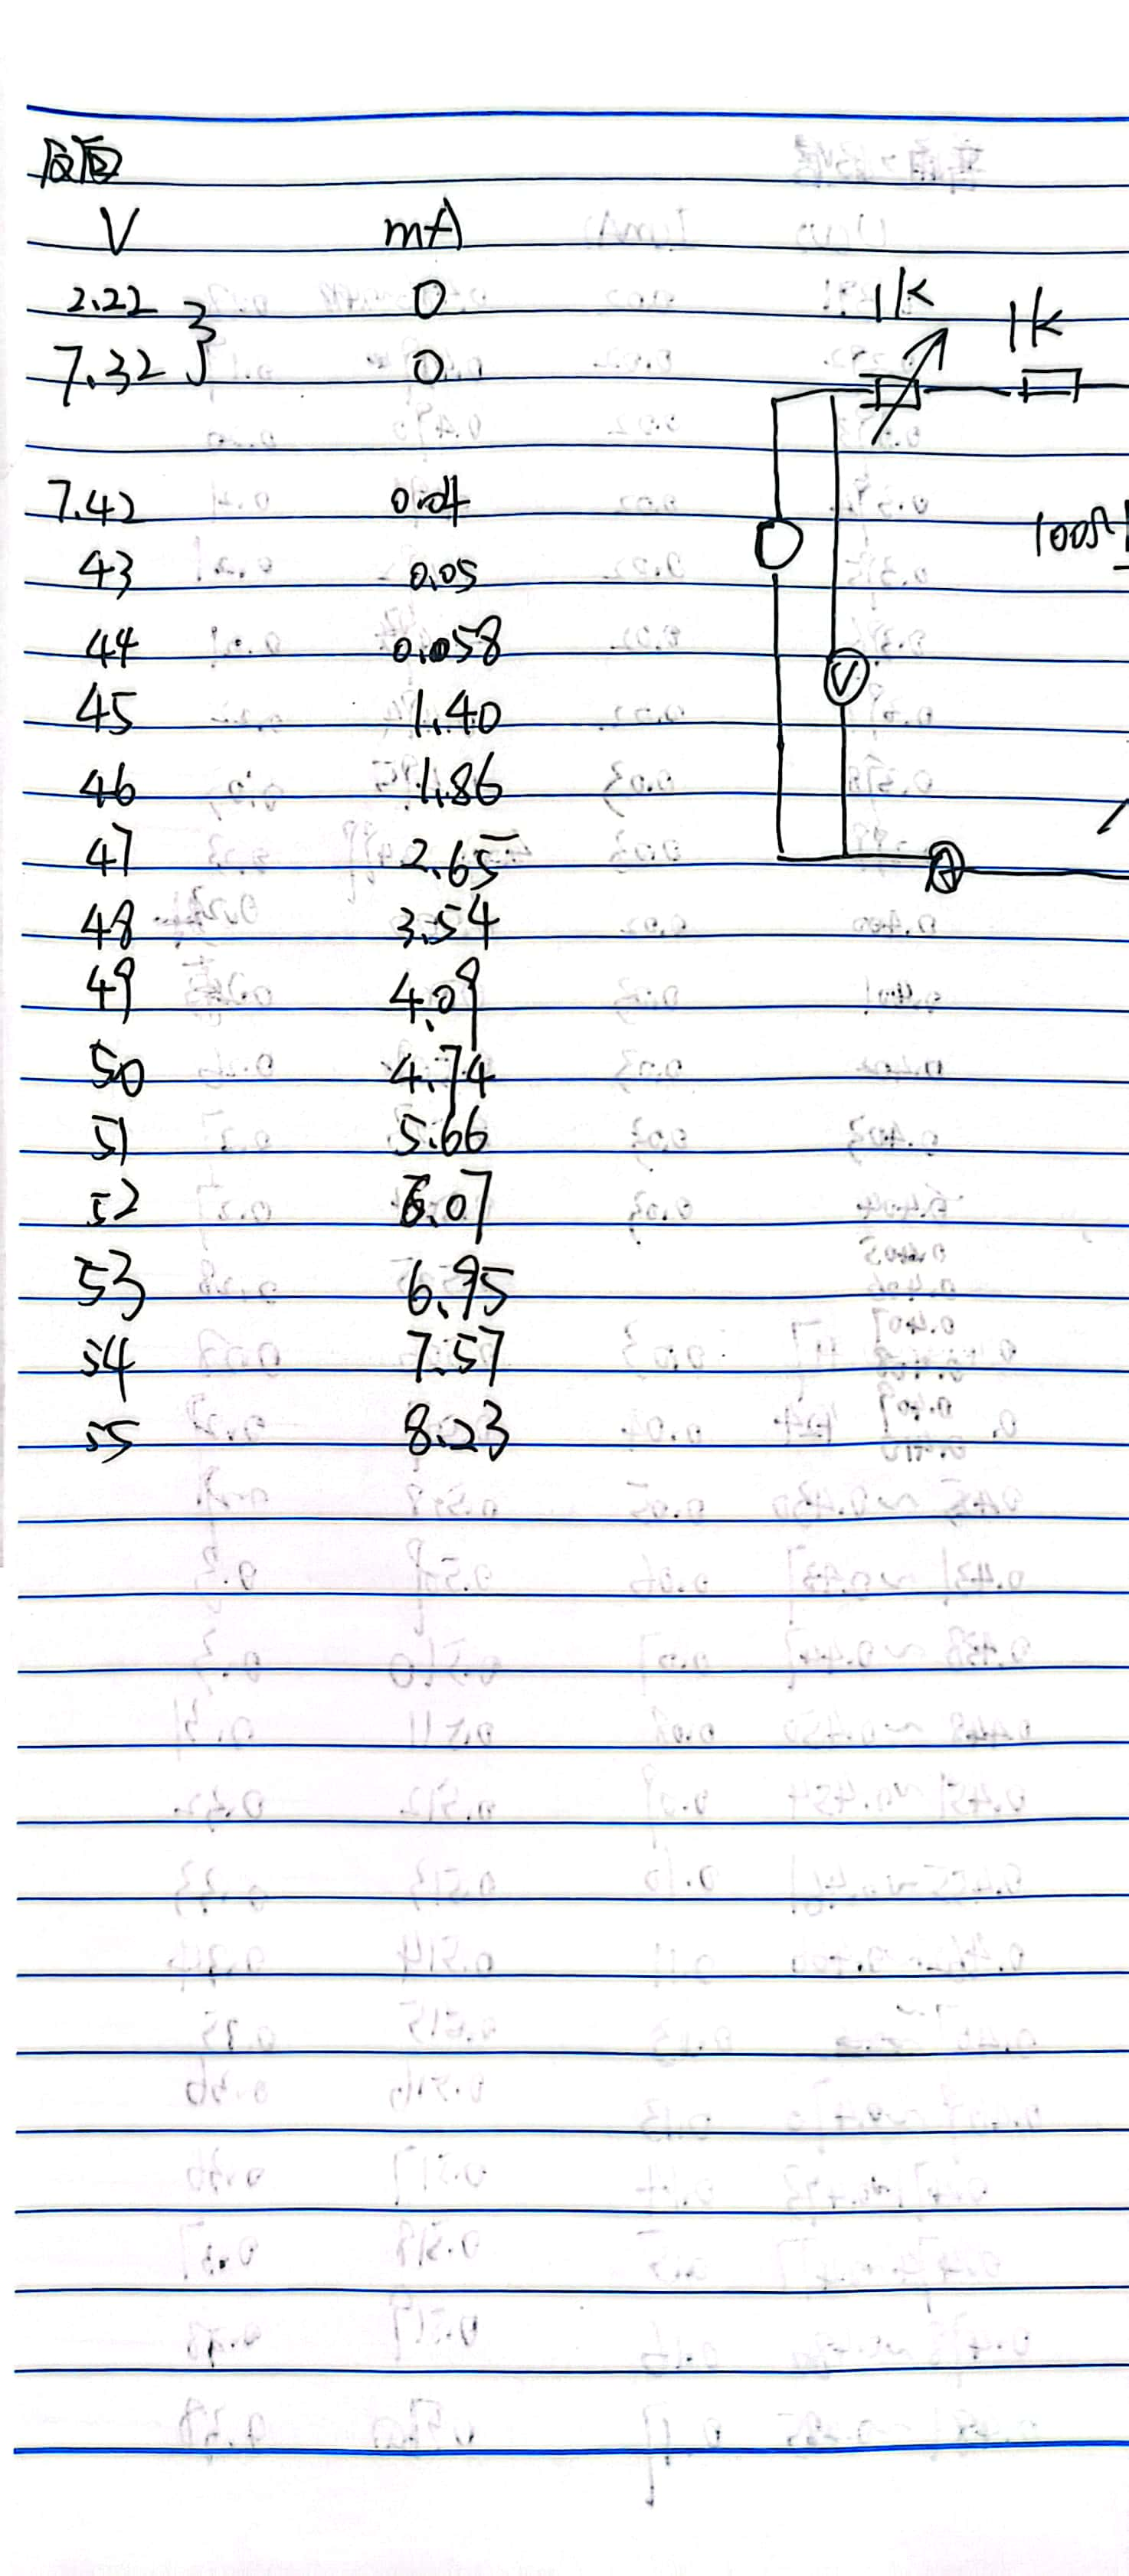
\includegraphics[width=1\textwidth,height=0.8\textheight]{wenyafanxiang.jpg}
  \caption{实验原始数据9}\label{wenyafanxiang}
\end{figure}
\newpage





\section{实验数据处理}
  \subsection{测量普通电阻通电后的伏安特性曲线}
  \begin{wrapfigure}[4]{l}{4cm}\label{dianzushujv}
    \centering
    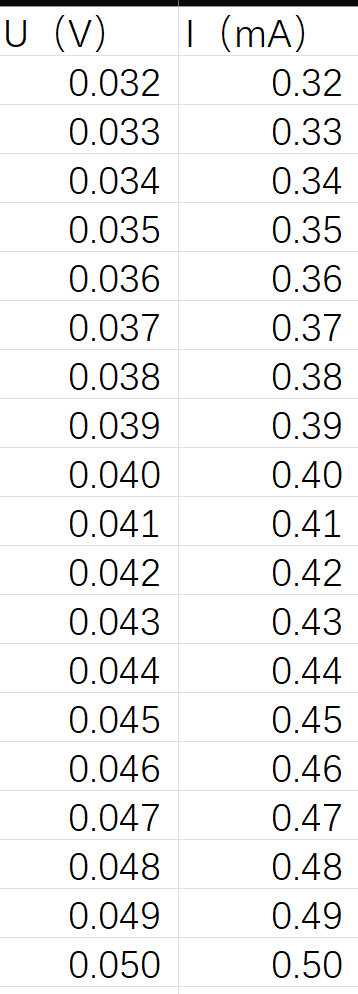
\includegraphics[width=0.1\textwidth,height=0.4\textheight]{dianzushujv.png}
    \caption{电阻数据}
  \end{wrapfigure}

  实验中测得的电阻导通数据如图\ref{dianzushujv}。对数据进行处理最终得到图\ref{dianzuzuotu}。

  \begin{figure}[H]\label{dianzuzuotu}
    \centering
    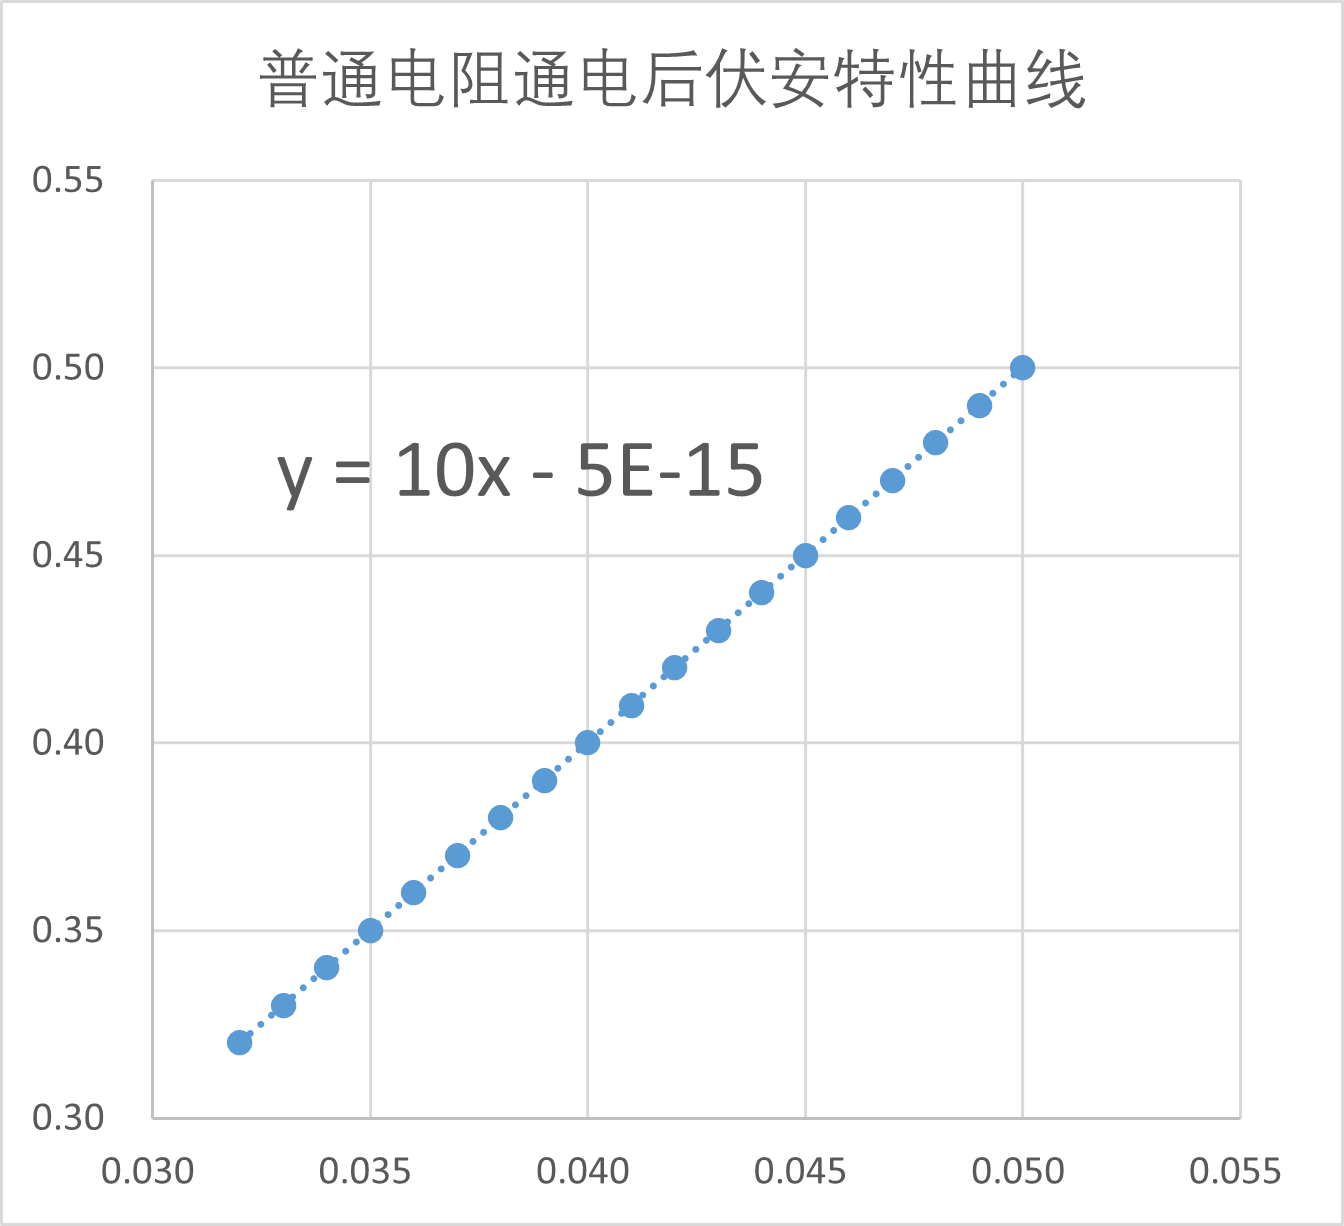
\includegraphics[width=0.4\textwidth,height=0.3\textheight]{dianzuzuotu.png}
    \caption{电阻结果作图}
  \end{figure}

  最终得到的实验结果较为满意,基本符合欧姆定律,可能由于测量时间较短,所以电阻发热不严重没有
  影响其阻值,得到的伏安特性曲线也是较为完美的直线。实验较为成功。

  \subsection{测量普通二极管的正向伏安特性曲线}
  \begin{wrapfigure}[2]{l}{4cm}\label{putongshujv}
    \centering
    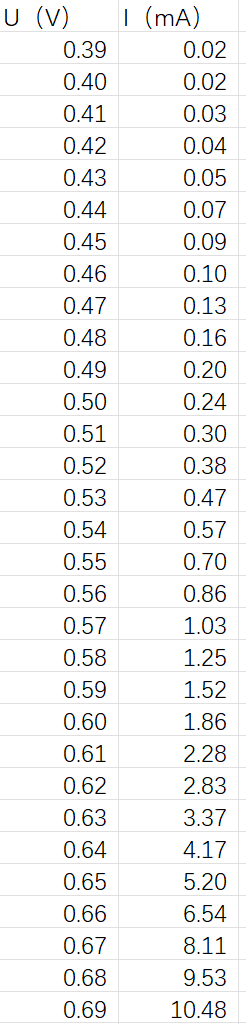
\includegraphics[width=0.1\textwidth,height=0.3\textheight]{putongshujv.png}
    \caption{普通二极管数据}
  \end{wrapfigure}

  实验中测得的普通二极管
  伏安特性曲线数据如图\ref{putongshujv}。对数据进行处理最终得到图\ref{putongzuotu}。

  \begin{figure}[H]\label{putongzuotu}
    \centering
    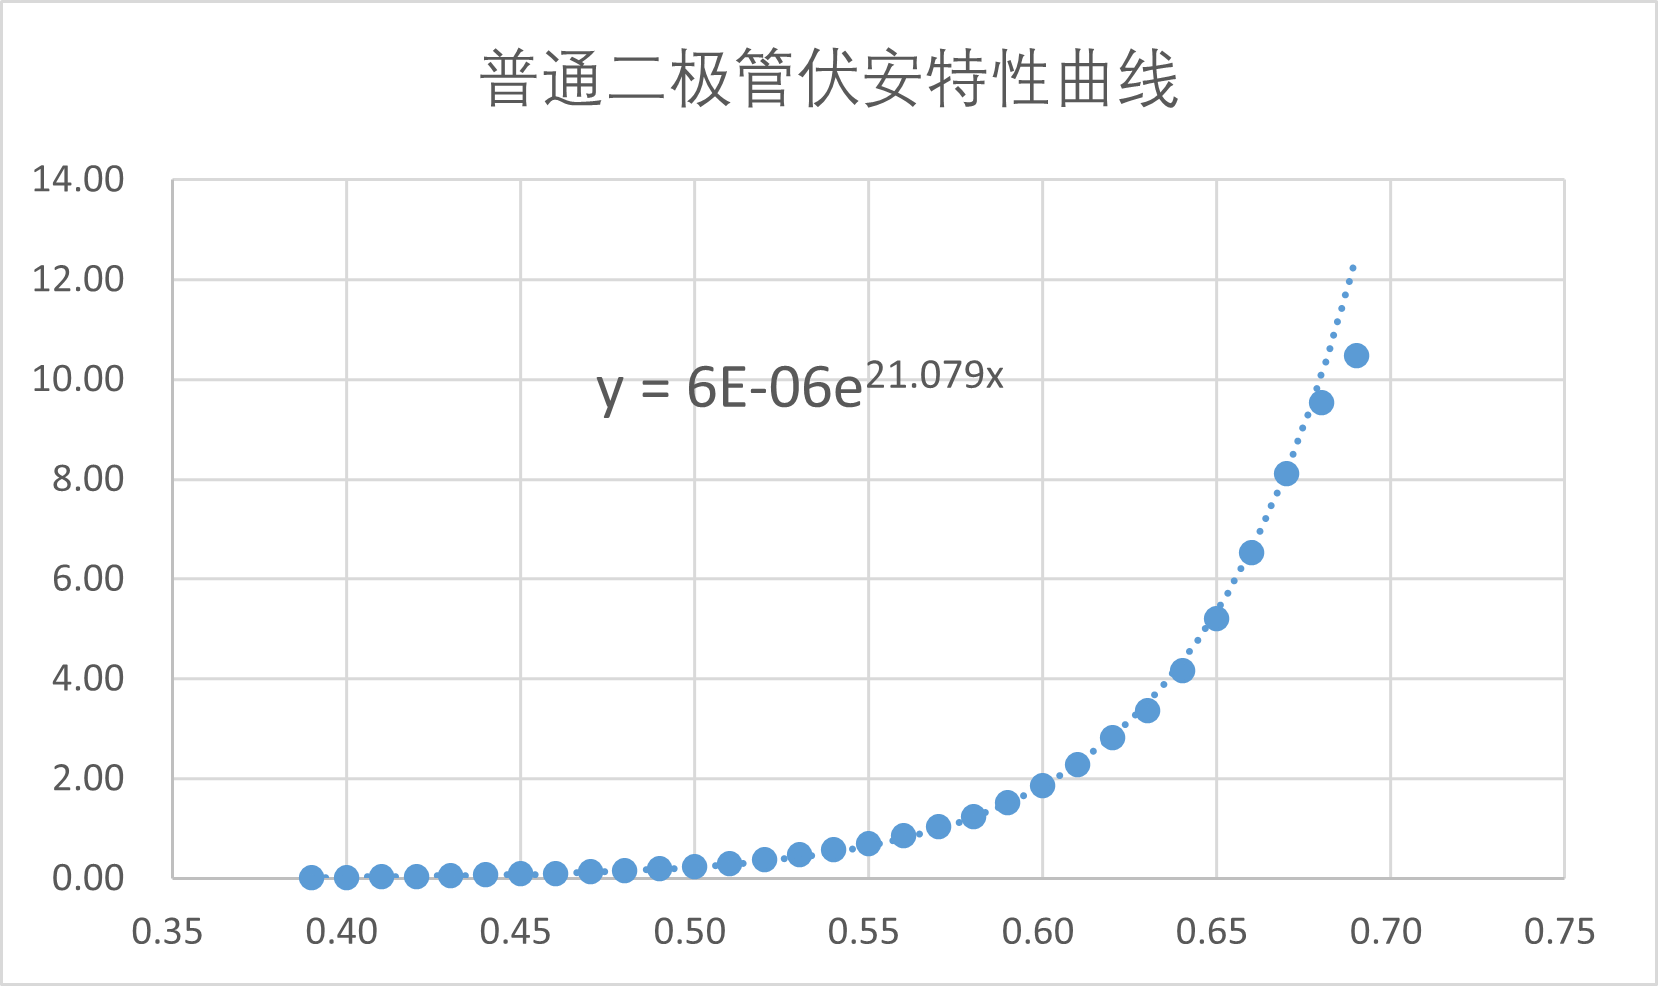
\includegraphics[width=0.4\textwidth,height=0.3\textheight]{putongzuotu.png}
    \caption{普通二极管伏安特性曲线作图}
  \end{figure}

  最终得到的实验结果表明整个实验数据得到的图形基本符合非线性元件的e为底的指数曲线拟合结果。
  \subsection{测量稳压二极管伏安特性曲线}
  实验包括两部分,一部分是正向导通的情况下的伏安特性曲线,另一部分是反向导通的情况下的伏安特性曲线。
  
  \subsubsection{测量稳压二极管的正向伏安特性曲线}

  \begin{wrapfigure}[4]{l}{4cm}\label{wenyazhengxiangshujv}
    \centering
    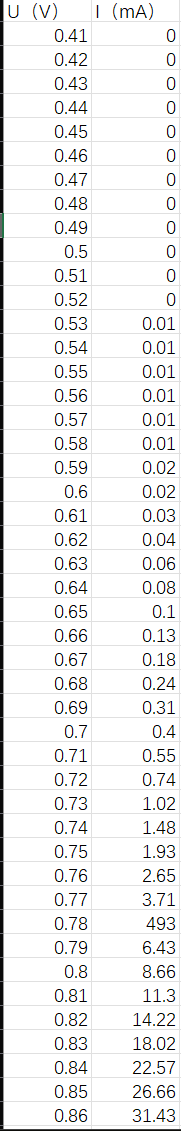
\includegraphics[width=0.1\textwidth,height=0.4\textheight]{wenyazhengxiangshujv.png}
    \caption{稳压二极管正向导通数据}
  \end{wrapfigure}
  实验中测得的稳压二极管正向导通的时候的
  伏安特性曲线数据如图\ref{wenyazhengxiangshujv}。对数据进行处理最终得到图\ref{wenyazhengxiangzuotu}。
  \begin{figure}[H]\label{wenyazhengxiangzuotu}
    \centering
    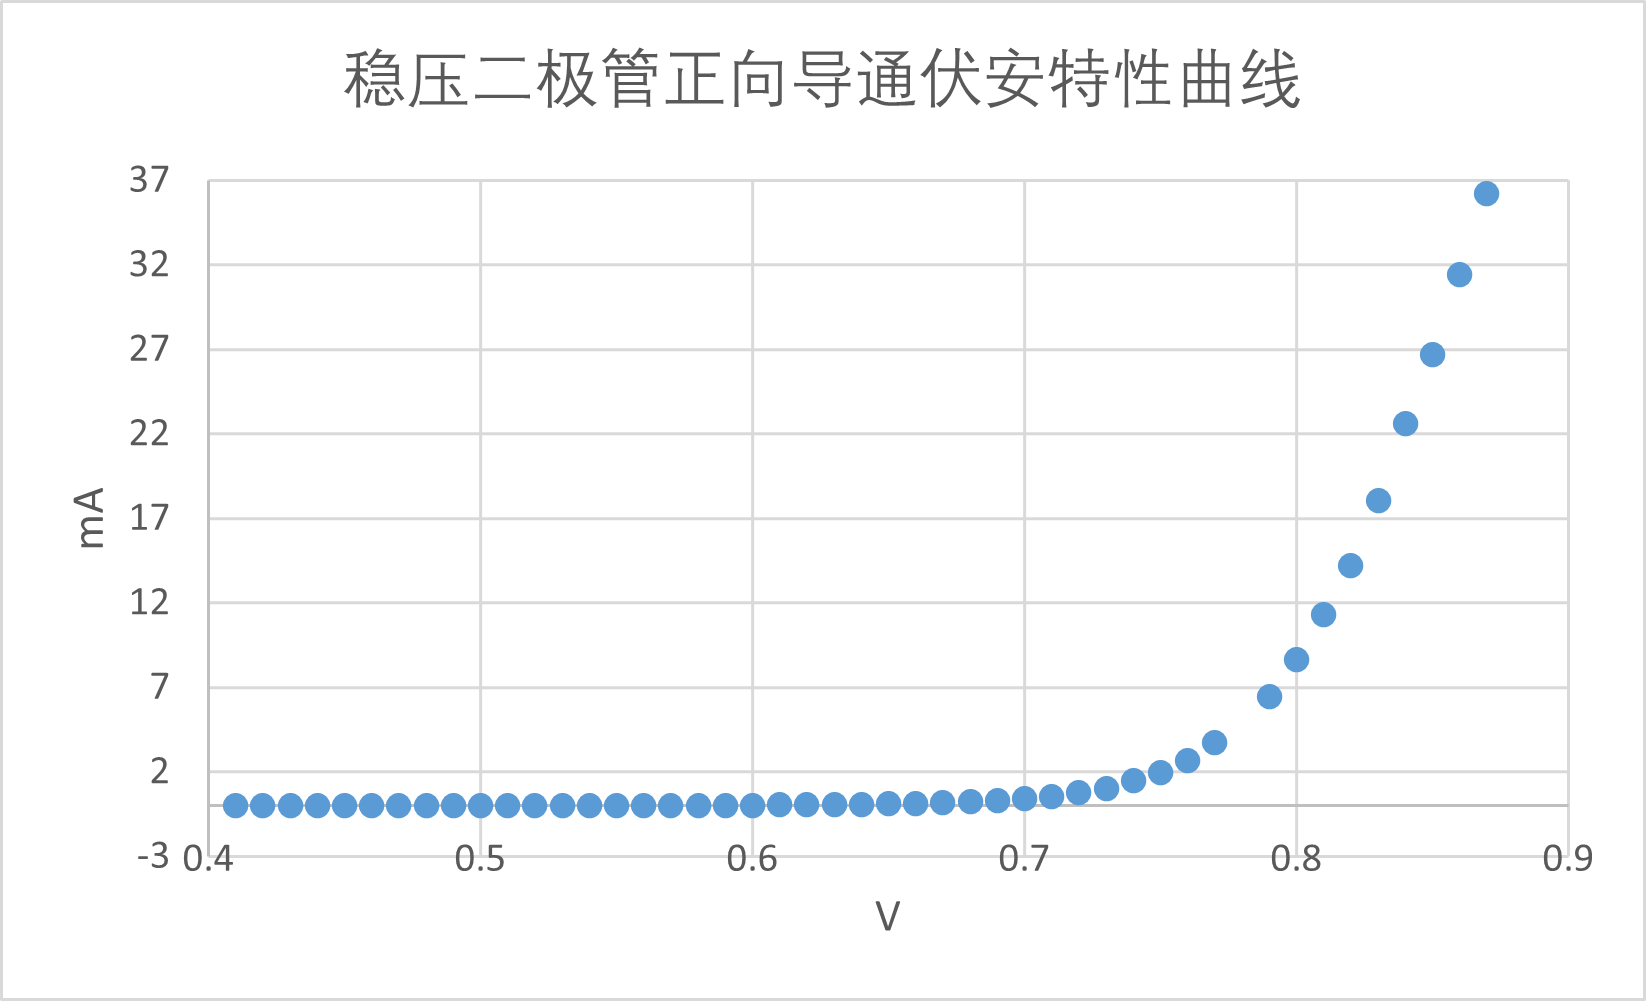
\includegraphics[width=0.4\textwidth,height=0.3\textheight]{wenyazhengxiangzuotu.png}
    \caption{稳压二极管正向导通伏安特性曲线作图}
  \end{figure}

  \subsubsection{测量稳压二极管的反向伏安特性曲线}

  \begin{wrapfigure}[3]{l}{4cm}\label{wenyafanxiangshujv}
    \centering
    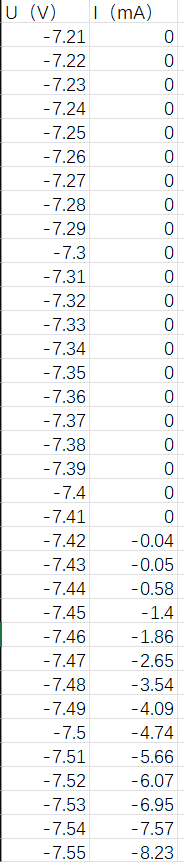
\includegraphics[width=0.3\textwidth,height=0.4\textheight]{wenyafanxiangshujv.png}
    \caption{稳压二极管反向导通数据}
  \end{wrapfigure}
  实验中测得的稳压二极管反向导通的时候的
  伏安特性曲线数据如图\ref{wenyafanxiangshujv}。对数据进行处理最终得到图\ref{wenyafanxiangzuotu}。
  \newpage
  \begin{figure}[h]\label{wenyafanxiangzuotu}
    \centering
    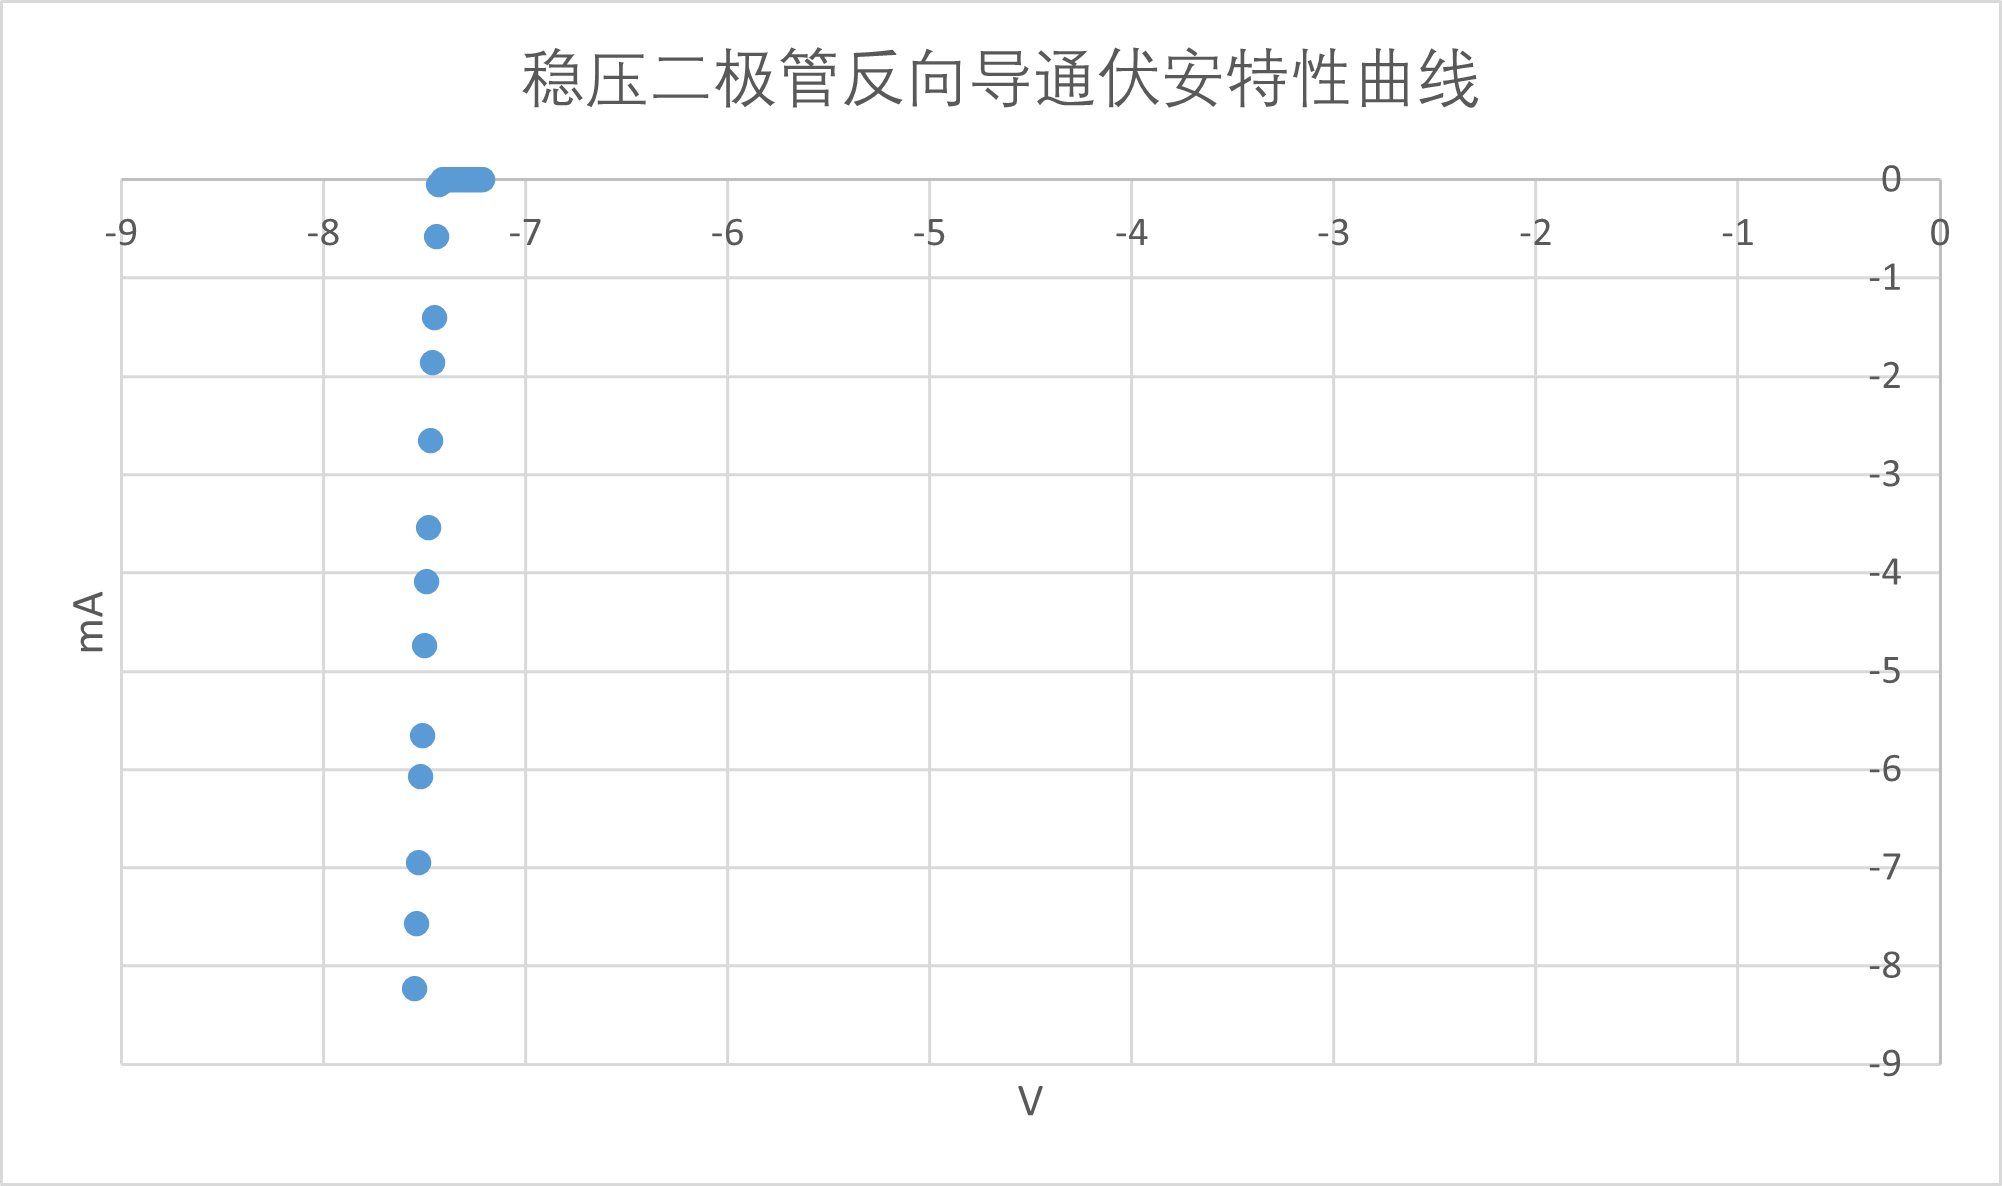
\includegraphics[width=0.4\textwidth,height=0.3\textheight]{wenyafanxiangzuotu.png}
    \caption{稳压二极管反向导通伏安特性曲线作图}
  \end{figure}

  从实验结果和数据处理后形成的图像观察可以得出无论是正向导通还是反向导通,稳压二极管
  曲线的趋势和普通二极管正向导通时候的图像是相似的,而具体而言,正向导通的导通电压阈值
  相较于反向导通的导通电压阈值要小很多,这也体现了二极管单向导通的性质,即便是稳压二极管上
  仍有体现。并且稳压二极管的曲线更加陡,相同电压变化下电流变化更大。
\newpage

  \subsection{测量发光二极管的正向伏安特性曲线}
  \begin{figure}[H]\label{ledshujv}
    \centering
    \begin{minipage}{\textwidth}
    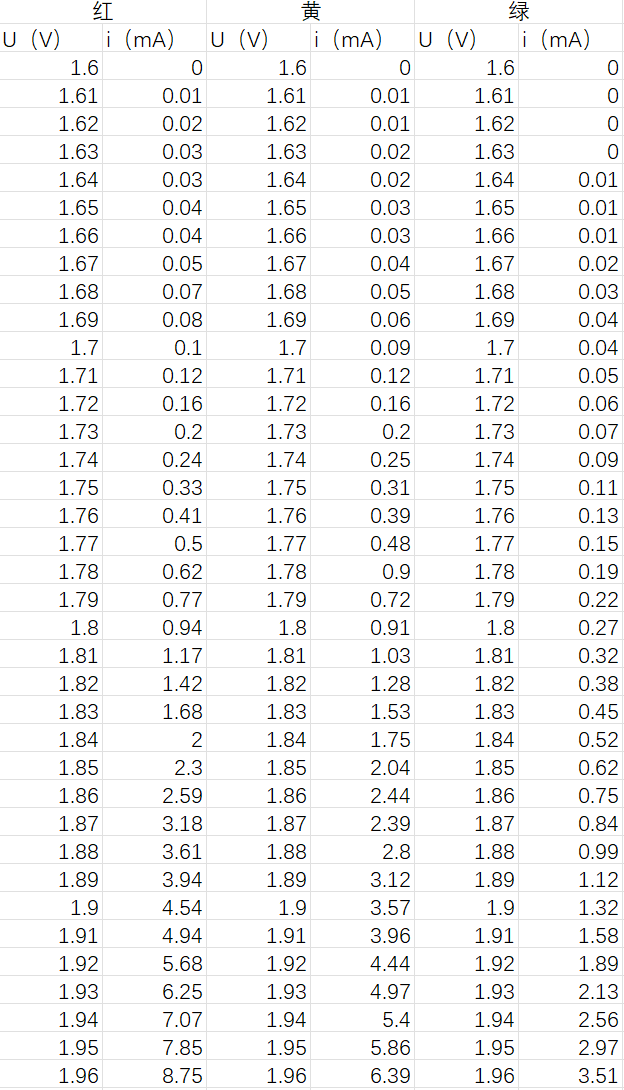
\includegraphics[width=0.2\textwidth,height=0.5\textheight]{ledshujv.png}
    \end{minipage}
    \caption{LED灯数据}
  \end{figure}
    实验中测得的LED灯的
  伏安特性曲线数据如图\ref{ledshujv}。对数据进行处理最终得到图\ref{ledzuotu}。
  \begin{figure}[H]\label{ledzuotu}
    \centering
    \begin{minipage}{\linewidth}
    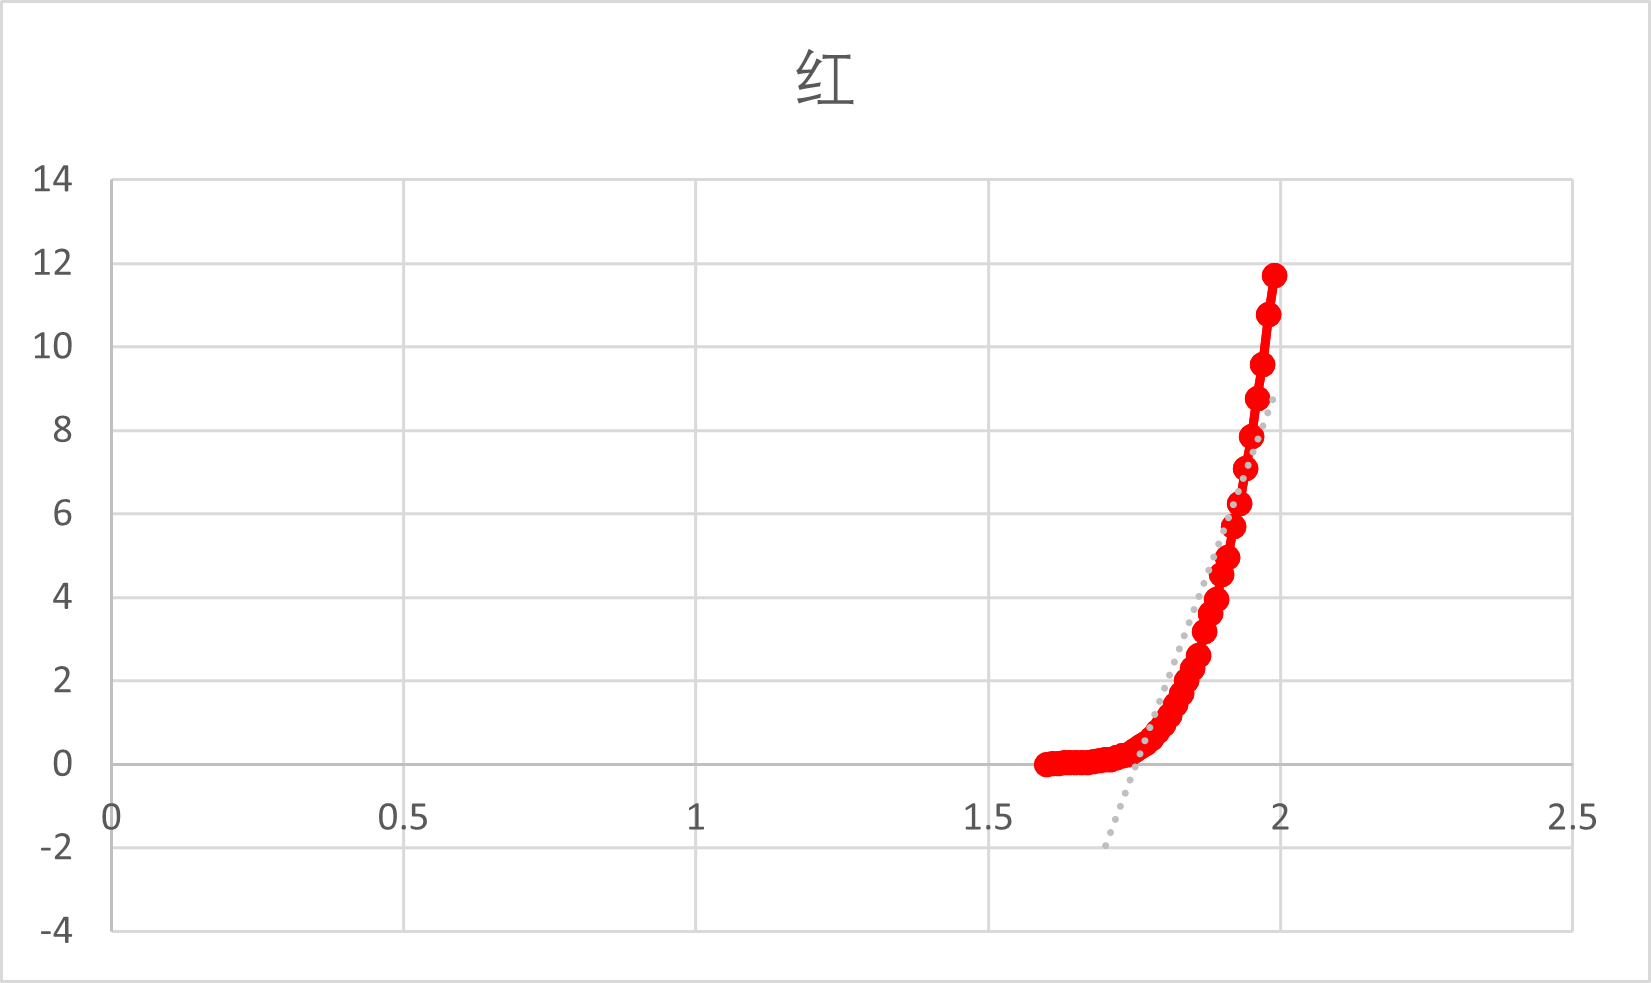
\includegraphics[width=0.47\textwidth,height=0.3\textheight]{ledzuotu1.png}\hfill
    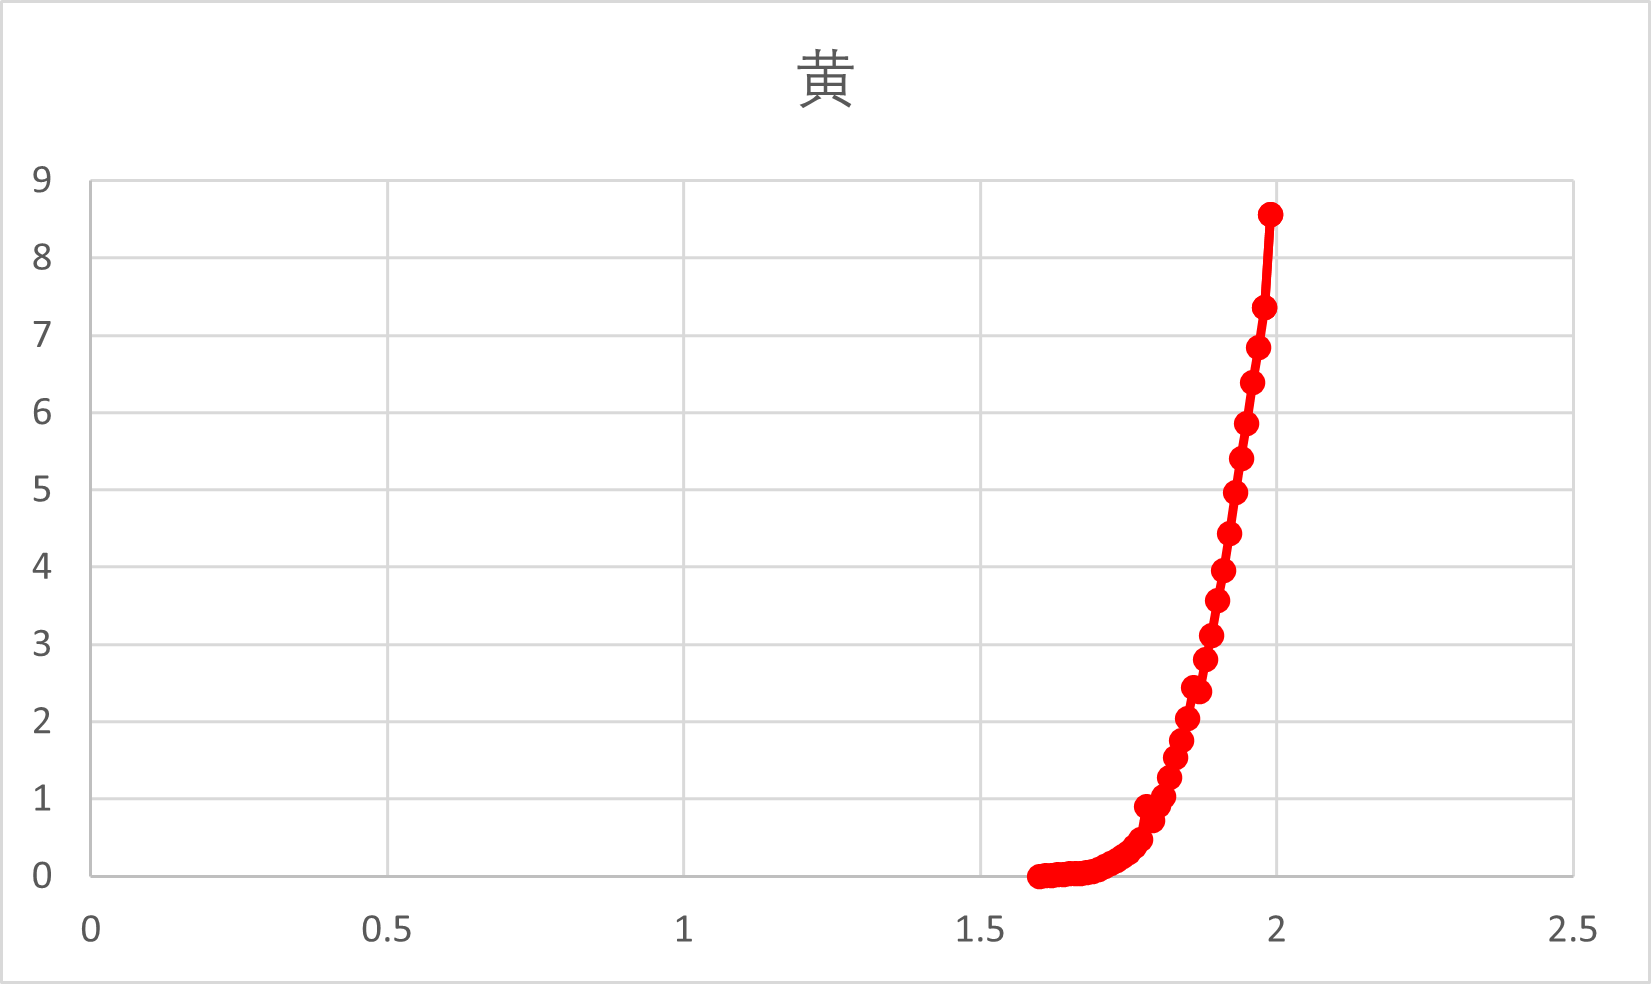
\includegraphics[width=0.47\textwidth,height=0.3\textheight]{ledzuotu2.png}\hfill
    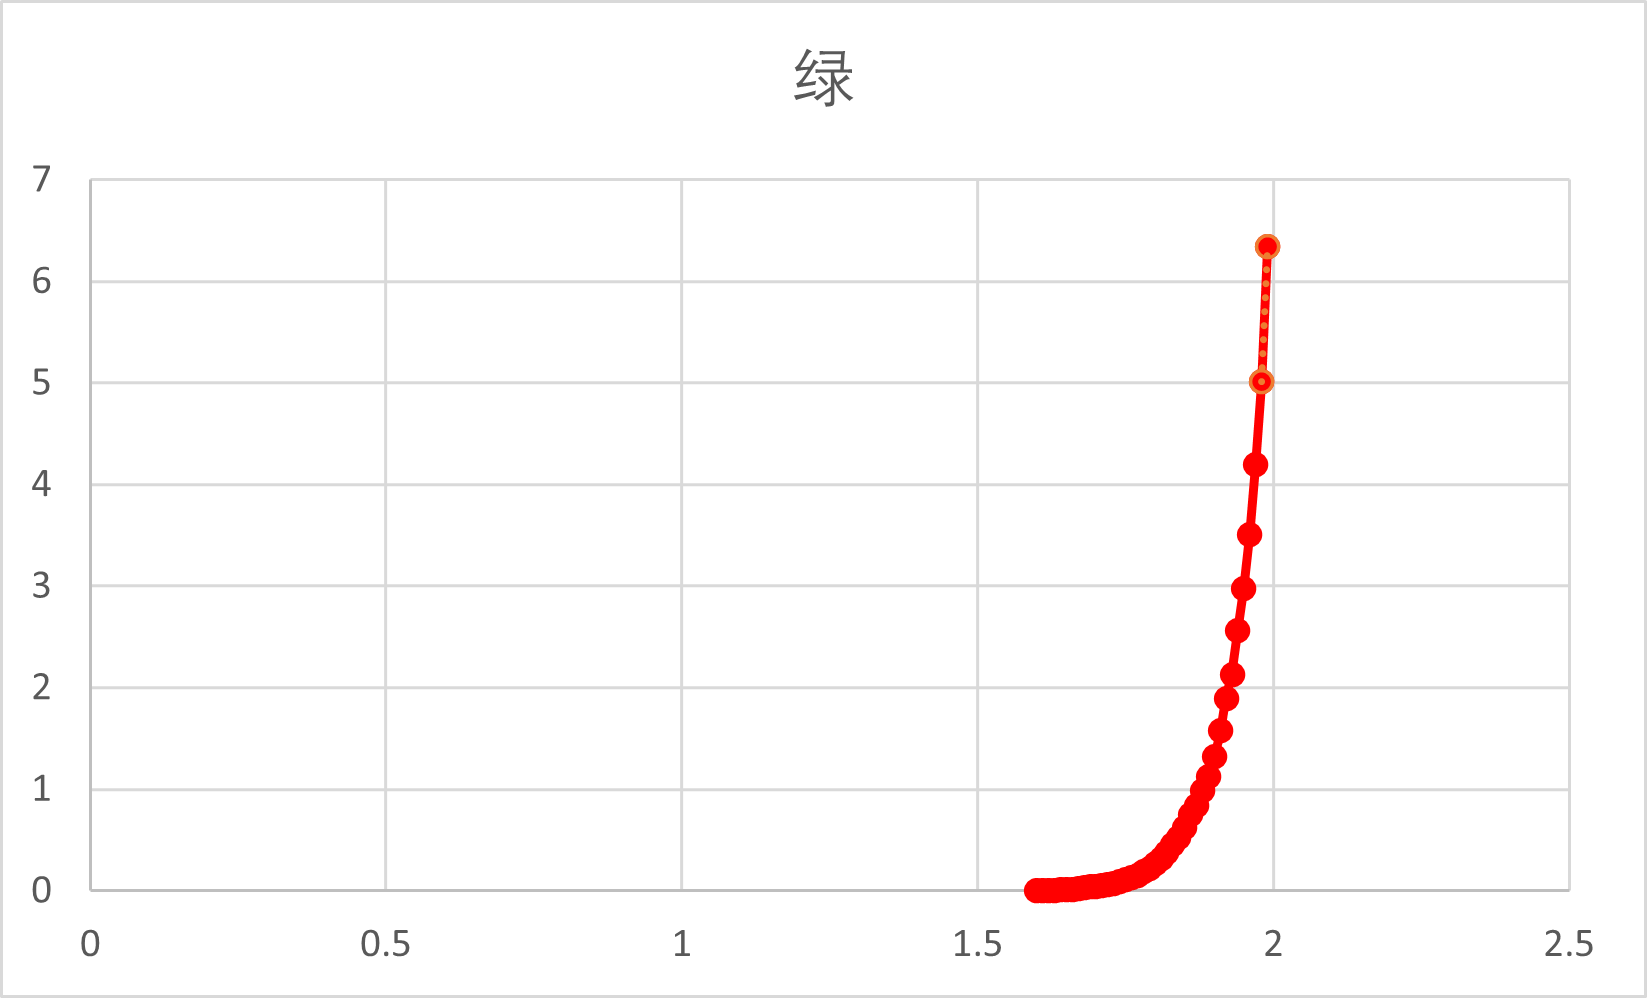
\includegraphics[width=0.47\textwidth,height=0.3\textheight]{ledzuotu3.png}
    \end{minipage}
    \caption{LED灯作图结果}
  \end{figure}

  从实验结果和数据处理后形成的图像观察可以得出无论哪种颜色的发光半导体最终产生的曲线
  依旧和普通二极管的伏安特性曲线相似。而不同颜色的二极管的导通后的倾斜趋势不同,这也
  体现在不同二极管的所需要的导通电压阈值不同。通过计算最终得到的灯管的波长如下表\ref{bochang}

  \begin{table}[h]
    \centering   
    \caption{不同LED灯管发光波长计算}\label{bochang}
    \begin{tabular}{| l || l |}
        \hline
        发光灯管颜色 & 波长数值\\
        \hline
        红色 & 707.567 \\
        \hline
        黄色 & 676.687 \\
        \hline
        绿色 & 644.808 \\
        \hline
    \end{tabular}
  \end{table}

  最终得到的结果误差较大,出现明显向红光偏移的趋势,分析误差产生原因:

  1.  二极管发热导致伏安特性曲线不是相同状态下测得的

  2.  二极管发光的时候也有红光产生,但是由于灯罩原因滤掉红光

  3.  二极管出现故障,或者仪器误差

  4.  测量过程中未等待二极管达到稳定工作状态就记录数据

\section{思考题}
  \subsection{思考题二}
  可以通过实验数据并进行拟合后得到曲线公式,此公式就是经验公式。
  \subsection{思考题三}
  可以直接检测光谱和光强,然后就能得出峰值波长。同样也可以使用
  双缝干涉类似的实验通过测量干涉图像数据通过计算得到峰值波长。
  \subsection{思考题四}
  使用示波器直接显示稳压二极管的伏安特性曲线还需要可变直流电源,该电源
  还需要能够改变电流方向。同时,还需要示波器一台。电路连接:
  将直流电源的正极连接到稳压二极管的阳极。
  再将直流电源的负极连接到稳压二极管的阴极。
  连接一个限制电流的电阻到稳压二极管的阴极,然后将另一端连接到直流电源的负极。
  连接示波器的探头,一个连接到稳压二极管的阳极,另一个连接到电阻和直流电源之间的连接点。

  然后控制直流电源,逐步增加电流大小,注意记录数据点位置。

  实验中通过调节电流源来控制通过二极管的电流。在实验中需要注意电流大小变化不能太大。

\section{实验中个人的思考与感想}
  \subsection{对于实验个人观点}
  实验通过这种描点的方法来得到二极管的伏安特性曲线,这种方法也是非常常见的。
  实际实验中的电路和书上的电路时不太一样的,所以实验中也无法得到书上要求的0V的电压数据,
  都是从零点几的电压开始调节。实验中可以有限压和限流两个旋钮进行调节二极管两侧分得电压,
  其中限压的控制更加大范围,而限流是在限压的基础上进行控制的。这可以避免电压过大,也方便
  实验中控制电压。

  实验中二极管会发热,在使用了一段时间以后二极管温度会有所上升,虽然不大,但是总是有些
  发热,所以还是会对实验中的数据测量产生误差。

  同样实验中一个电路做完所有实验也存在一定不合理性,因为不同二极管的导通电压阈值是不同的,
  导通后的曲线也是不同的,所以可能出现实验中对于某个二极管合适,但是对于另一个二极管电压
  太小或者太大的问题,这也是无法达到0V带来的问题。并且实验中在测量的时候经常会出现处在某个
  范围电压的时候电流一直跳动的情况,这也会读数产生很大影响,很难确定具体数据哪个更合适。
  \subsection{实验中的总结}
  小幅度调节电压,测量电压和电流数据,将数据记录并作图,得到伏安特性曲线。
  实验中需要注意等待电流数据稳定,读数也要注意数据跳动不停的问题,还有要尽量大范围测量
  二极管数据,在能使二极管正常工作的前提下尽量扩大电压调节的范围。
\end{document}
